\chapter{Results}
\label{cha:results}

This chapter presents the results comparing our two deep RL agents to baseline and human-controlled agents.
In addition to the results here, learning curves for all environments are shown in Appendix~\ref{app:learning},
Some sample search path for our agents and baselines are shown in Appendix~\ref{app:paths}.

% todo: We can visualize attention as in "A critical investigation of deep reinforcement learning for navigation"

\section{Search Performance and Behavior}

Table~\ref{tab:metrics} shows the average search path length, success rate and SPL metric on a fixed set of 100 levels from each environment.
The average search path length is computed from episodes in which the agents successfully finds all targets.
These metrics are presented for our two agents trained on the full distribution of environments, as well as for the baselines and human searchers.
Appendix~\ref{app:learning} contains learning curves for each environment, and Appendix~\ref{app:paths} contains example search paths from each baseline and learning agent. 

Overall, our two agents and human searchers achieve similar success rates, path lengths and SPL scores.
Our spatial memory agent achieves the most competitive search path lengths and SPL scores in the Gaussian and terrain environments.
Our temporal memory agent select search paths that are on average longer than the paths chosen by our spatial memory agent and human searchers.
In the camera environment, the temporal memory agent is better both in terms of average length and SPL score.
Interestingly, the temporal memory agent achieves SPL scores comparable to that of the spatial memory agent despite choosing much longer path lengths.

Human searchers seemed to be successful in utilizing using environment cues to guide search, but frequently forgot which positions had been visited.
In the camera environment, human searchers found it difficult to identify when targets should be indicated,
as the discretization of the search space did not always align targets closely to the center of the screen.
This is more of a side effect of the implementation than an indication of poor search performance.

The random baseline policy achieves the worst SPL, success rate and average search path length in all three environments.
The greedy baseline policy is closer to the remaining agents.
The exhaustive baseline policy achieves an average search path length that is lower than our temporal memory agent.
Its SPL score, however, is only higher than the those of the other two baselines.
The handcrafted baseline for the Gaussian environment performed better than all other agents in this environment. % todo

\begin{table}
    \centering
    \label{tab:metrics}
    \caption[Performance metrics for each environment.]{SPL, success rate and average search path length on successful episodes from three runs on a fixed set of a 100 samples from each environment.}
    Gaussian environment\par\vspace{0.5em}
    \begin{tabular}{lccc}
    \toprule
    Agent & SPL & Success & Length \\
    \midrule
    random & $0.06 \pm 0.01$ & $0.92 \pm 0.06$ & $369.07 \pm 24.93$\\
    greedy & $0.17 \pm 0.00$ & $1.00 \pm 0.00$ & $147.12 \pm 2.38$\\
    exhaustive & $0.21 \pm 0.00$ & $1.00 \pm 0.00$ & $83.37 \pm 2.88$\\
    handcrafted & $0.33 \pm 0.00$ & $1.00 \pm 0.00$ & $65.20 \pm 1.41$\\
    human & $0.23 \pm 0.03$ & $1.00 \pm 0.00$ & $80.97 \pm 13.49$\\
    temporal & $0.24 \pm 0.03$ & $0.99 \pm 0.01$ & $101.25 \pm 13.32$\\
    spatial & $0.29 \pm 0.02$ & $0.99 \pm 0.01$ & $72.16 \pm 5.97$\\
    \bottomrule
\end{tabular}

    \par\vspace{1em}Terrain environment\par\vspace{0.5em}
    \begin{tabular}{lccc}
    \toprule
    Agent & SPL & Success & Length \\
    \midrule
    random & $0.06 \pm 0.01$ & $0.89 \pm 0.04$ & $366.05 \pm 26.96$\\
    greedy & $0.17 \pm 0.01$ & $1.00 \pm 0.00$ & $141.01 \pm 2.31$\\
    exhaustive & $0.22 \pm 0.00$ & $1.00 \pm 0.00$ & $84.11 \pm 0.84$\\
    human & $0.26 \pm 0.02$ & $1.00 \pm 0.00$ & $76.73 \pm 5.33$\\
    \midrule
    temporal & $0.25 \pm 0.02$ & $1.00 \pm 0.01$ & $103.76 \pm 11.69$\\
    spatial & $0.27 \pm 0.01$ & $1.00 \pm 0.00$ & $79.60 \pm 6.88$\\
    \bottomrule
\end{tabular}
    \par\vspace{1em}Camera environment\par\vspace{0.5em}
    \begin{tabular}{lccc}
    \toprule
    Agent & SPL & Success & Length \\
    \midrule
    random & $0.04 \pm 0.00$ & $0.62 \pm 0.03$ & $545.09 \pm 56.25$\\
    greedy & $0.12 \pm 0.01$ & $0.97 \pm 0.01$ & $255.60 \pm 10.44$\\
    exhaustive & $0.37 \pm 0.00$ & $1.00 \pm 0.00$ & $67.03 \pm 0.00$\\
    human & $0.68 \pm 0.08$ & $1.00 \pm 0.00$ & $38.10 \pm 5.72$\\
    \midrule
    temporal & $0.70 \pm 0.02$ & $1.00 \pm 0.00$ & $42.36 \pm 2.05$\\
    spatial & $0.66 \pm 0.03$ & $1.00 \pm 0.00$ & $42.90 \pm 1.73$\\
    \bottomrule
\end{tabular}
\end{table}

\section{Size of Search Space}
\label{sec:shape}

The results of the search space experiments in the Gaussian environment are presented in Figure~\ref{fig:shape}.
Results were collected across four different runs, and the plots show the mean and standard deviation.
For the search space of \(10 \times 10\), both architectures initially improve their policy quickly.
Past a certain time step, they keep improving at a reduced pace.
At the end of training, the spatial memory architecture has reached a policy that seems to find targets quicker than the temporal memory.
Both seem to be able to find all three targets in every episode.

For the larger search space sizes with \(15 \times 15\) and \(20 \times 20\) the difference between the two architectures is greater.
While the spatial memory seems to consistently find targets in a number of steps that is comparable to the number of positions in the search space,
the search paths of the agent with the temporal memory are substantially longer.
Furthermore, the variance across runs increases with the search space size.

\begin{figure}
    \centering
    \(10 \times 10\)
    %% Creator: Matplotlib, PGF backend
%%
%% To include the figure in your LaTeX document, write
%%   \input{<filename>.pgf}
%%
%% Make sure the required packages are loaded in your preamble
%%   \usepackage{pgf}
%%
%% Also ensure that all the required font packages are loaded; for instance,
%% the lmodern package is sometimes necessary when using math font.
%%   \usepackage{lmodern}
%%
%% Figures using additional raster images can only be included by \input if
%% they are in the same directory as the main LaTeX file. For loading figures
%% from other directories you can use the `import` package
%%   \usepackage{import}
%%
%% and then include the figures with
%%   \import{<path to file>}{<filename>.pgf}
%%
%% Matplotlib used the following preamble
%%   \usepackage{fontspec}
%%   \setmainfont{DejaVuSerif.ttf}[Path=\detokenize{/home/oslund/.local/lib/python3.8/site-packages/matplotlib/mpl-data/fonts/ttf/}]
%%   \setsansfont{DejaVuSans.ttf}[Path=\detokenize{/home/oslund/.local/lib/python3.8/site-packages/matplotlib/mpl-data/fonts/ttf/}]
%%   \setmonofont{DejaVuSansMono.ttf}[Path=\detokenize{/home/oslund/.local/lib/python3.8/site-packages/matplotlib/mpl-data/fonts/ttf/}]
%%
\begingroup%
\makeatletter%
\begin{pgfpicture}%
\pgfpathrectangle{\pgfpointorigin}{\pgfqpoint{5.645496in}{3.489108in}}%
\pgfusepath{use as bounding box, clip}%
\begin{pgfscope}%
\pgfsetbuttcap%
\pgfsetmiterjoin%
\definecolor{currentfill}{rgb}{1.000000,1.000000,1.000000}%
\pgfsetfillcolor{currentfill}%
\pgfsetlinewidth{0.000000pt}%
\definecolor{currentstroke}{rgb}{1.000000,1.000000,1.000000}%
\pgfsetstrokecolor{currentstroke}%
\pgfsetdash{}{0pt}%
\pgfpathmoveto{\pgfqpoint{0.000000in}{0.000000in}}%
\pgfpathlineto{\pgfqpoint{5.645496in}{0.000000in}}%
\pgfpathlineto{\pgfqpoint{5.645496in}{3.489108in}}%
\pgfpathlineto{\pgfqpoint{0.000000in}{3.489108in}}%
\pgfpathlineto{\pgfqpoint{0.000000in}{0.000000in}}%
\pgfpathclose%
\pgfusepath{fill}%
\end{pgfscope}%
\begin{pgfscope}%
\pgfsetbuttcap%
\pgfsetmiterjoin%
\definecolor{currentfill}{rgb}{1.000000,1.000000,1.000000}%
\pgfsetfillcolor{currentfill}%
\pgfsetlinewidth{0.000000pt}%
\definecolor{currentstroke}{rgb}{0.000000,0.000000,0.000000}%
\pgfsetstrokecolor{currentstroke}%
\pgfsetstrokeopacity{0.000000}%
\pgfsetdash{}{0pt}%
\pgfpathmoveto{\pgfqpoint{0.602198in}{0.524170in}}%
\pgfpathlineto{\pgfqpoint{2.760816in}{0.524170in}}%
\pgfpathlineto{\pgfqpoint{2.760816in}{3.041514in}}%
\pgfpathlineto{\pgfqpoint{0.602198in}{3.041514in}}%
\pgfpathlineto{\pgfqpoint{0.602198in}{0.524170in}}%
\pgfpathclose%
\pgfusepath{fill}%
\end{pgfscope}%
\begin{pgfscope}%
\pgfsys@transformshift{0.700000in}{0.639108in}%
\pgftext[left,bottom]{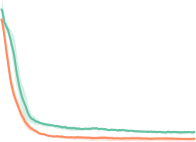
\includegraphics[interpolate=true,width=1.970000in,height=2.300000in]{shape-10-img0.png}}%
\end{pgfscope}%
\begin{pgfscope}%
\pgfsetbuttcap%
\pgfsetroundjoin%
\definecolor{currentfill}{rgb}{0.000000,0.000000,0.000000}%
\pgfsetfillcolor{currentfill}%
\pgfsetlinewidth{0.803000pt}%
\definecolor{currentstroke}{rgb}{0.000000,0.000000,0.000000}%
\pgfsetstrokecolor{currentstroke}%
\pgfsetdash{}{0pt}%
\pgfsys@defobject{currentmarker}{\pgfqpoint{0.000000in}{-0.048611in}}{\pgfqpoint{0.000000in}{0.000000in}}{%
\pgfpathmoveto{\pgfqpoint{0.000000in}{0.000000in}}%
\pgfpathlineto{\pgfqpoint{0.000000in}{-0.048611in}}%
\pgfusepath{stroke,fill}%
}%
\begin{pgfscope}%
\pgfsys@transformshift{0.674204in}{0.524170in}%
\pgfsys@useobject{currentmarker}{}%
\end{pgfscope}%
\end{pgfscope}%
\begin{pgfscope}%
\definecolor{textcolor}{rgb}{0.000000,0.000000,0.000000}%
\pgfsetstrokecolor{textcolor}%
\pgfsetfillcolor{textcolor}%
\pgftext[x=0.674204in,y=0.426948in,,top]{\color{textcolor}\rmfamily\fontsize{8.000000}{9.600000}\selectfont \(\displaystyle {0.0}\)}%
\end{pgfscope}%
\begin{pgfscope}%
\pgfsetbuttcap%
\pgfsetroundjoin%
\definecolor{currentfill}{rgb}{0.000000,0.000000,0.000000}%
\pgfsetfillcolor{currentfill}%
\pgfsetlinewidth{0.803000pt}%
\definecolor{currentstroke}{rgb}{0.000000,0.000000,0.000000}%
\pgfsetstrokecolor{currentstroke}%
\pgfsetdash{}{0pt}%
\pgfsys@defobject{currentmarker}{\pgfqpoint{0.000000in}{-0.048611in}}{\pgfqpoint{0.000000in}{0.000000in}}{%
\pgfpathmoveto{\pgfqpoint{0.000000in}{0.000000in}}%
\pgfpathlineto{\pgfqpoint{0.000000in}{-0.048611in}}%
\pgfusepath{stroke,fill}%
}%
\begin{pgfscope}%
\pgfsys@transformshift{1.072164in}{0.524170in}%
\pgfsys@useobject{currentmarker}{}%
\end{pgfscope}%
\end{pgfscope}%
\begin{pgfscope}%
\definecolor{textcolor}{rgb}{0.000000,0.000000,0.000000}%
\pgfsetstrokecolor{textcolor}%
\pgfsetfillcolor{textcolor}%
\pgftext[x=1.072164in,y=0.426948in,,top]{\color{textcolor}\rmfamily\fontsize{8.000000}{9.600000}\selectfont \(\displaystyle {0.5}\)}%
\end{pgfscope}%
\begin{pgfscope}%
\pgfsetbuttcap%
\pgfsetroundjoin%
\definecolor{currentfill}{rgb}{0.000000,0.000000,0.000000}%
\pgfsetfillcolor{currentfill}%
\pgfsetlinewidth{0.803000pt}%
\definecolor{currentstroke}{rgb}{0.000000,0.000000,0.000000}%
\pgfsetstrokecolor{currentstroke}%
\pgfsetdash{}{0pt}%
\pgfsys@defobject{currentmarker}{\pgfqpoint{0.000000in}{-0.048611in}}{\pgfqpoint{0.000000in}{0.000000in}}{%
\pgfpathmoveto{\pgfqpoint{0.000000in}{0.000000in}}%
\pgfpathlineto{\pgfqpoint{0.000000in}{-0.048611in}}%
\pgfusepath{stroke,fill}%
}%
\begin{pgfscope}%
\pgfsys@transformshift{1.470123in}{0.524170in}%
\pgfsys@useobject{currentmarker}{}%
\end{pgfscope}%
\end{pgfscope}%
\begin{pgfscope}%
\definecolor{textcolor}{rgb}{0.000000,0.000000,0.000000}%
\pgfsetstrokecolor{textcolor}%
\pgfsetfillcolor{textcolor}%
\pgftext[x=1.470123in,y=0.426948in,,top]{\color{textcolor}\rmfamily\fontsize{8.000000}{9.600000}\selectfont \(\displaystyle {1.0}\)}%
\end{pgfscope}%
\begin{pgfscope}%
\pgfsetbuttcap%
\pgfsetroundjoin%
\definecolor{currentfill}{rgb}{0.000000,0.000000,0.000000}%
\pgfsetfillcolor{currentfill}%
\pgfsetlinewidth{0.803000pt}%
\definecolor{currentstroke}{rgb}{0.000000,0.000000,0.000000}%
\pgfsetstrokecolor{currentstroke}%
\pgfsetdash{}{0pt}%
\pgfsys@defobject{currentmarker}{\pgfqpoint{0.000000in}{-0.048611in}}{\pgfqpoint{0.000000in}{0.000000in}}{%
\pgfpathmoveto{\pgfqpoint{0.000000in}{0.000000in}}%
\pgfpathlineto{\pgfqpoint{0.000000in}{-0.048611in}}%
\pgfusepath{stroke,fill}%
}%
\begin{pgfscope}%
\pgfsys@transformshift{1.868083in}{0.524170in}%
\pgfsys@useobject{currentmarker}{}%
\end{pgfscope}%
\end{pgfscope}%
\begin{pgfscope}%
\definecolor{textcolor}{rgb}{0.000000,0.000000,0.000000}%
\pgfsetstrokecolor{textcolor}%
\pgfsetfillcolor{textcolor}%
\pgftext[x=1.868083in,y=0.426948in,,top]{\color{textcolor}\rmfamily\fontsize{8.000000}{9.600000}\selectfont \(\displaystyle {1.5}\)}%
\end{pgfscope}%
\begin{pgfscope}%
\pgfsetbuttcap%
\pgfsetroundjoin%
\definecolor{currentfill}{rgb}{0.000000,0.000000,0.000000}%
\pgfsetfillcolor{currentfill}%
\pgfsetlinewidth{0.803000pt}%
\definecolor{currentstroke}{rgb}{0.000000,0.000000,0.000000}%
\pgfsetstrokecolor{currentstroke}%
\pgfsetdash{}{0pt}%
\pgfsys@defobject{currentmarker}{\pgfqpoint{0.000000in}{-0.048611in}}{\pgfqpoint{0.000000in}{0.000000in}}{%
\pgfpathmoveto{\pgfqpoint{0.000000in}{0.000000in}}%
\pgfpathlineto{\pgfqpoint{0.000000in}{-0.048611in}}%
\pgfusepath{stroke,fill}%
}%
\begin{pgfscope}%
\pgfsys@transformshift{2.266043in}{0.524170in}%
\pgfsys@useobject{currentmarker}{}%
\end{pgfscope}%
\end{pgfscope}%
\begin{pgfscope}%
\definecolor{textcolor}{rgb}{0.000000,0.000000,0.000000}%
\pgfsetstrokecolor{textcolor}%
\pgfsetfillcolor{textcolor}%
\pgftext[x=2.266043in,y=0.426948in,,top]{\color{textcolor}\rmfamily\fontsize{8.000000}{9.600000}\selectfont \(\displaystyle {2.0}\)}%
\end{pgfscope}%
\begin{pgfscope}%
\pgfsetbuttcap%
\pgfsetroundjoin%
\definecolor{currentfill}{rgb}{0.000000,0.000000,0.000000}%
\pgfsetfillcolor{currentfill}%
\pgfsetlinewidth{0.803000pt}%
\definecolor{currentstroke}{rgb}{0.000000,0.000000,0.000000}%
\pgfsetstrokecolor{currentstroke}%
\pgfsetdash{}{0pt}%
\pgfsys@defobject{currentmarker}{\pgfqpoint{0.000000in}{-0.048611in}}{\pgfqpoint{0.000000in}{0.000000in}}{%
\pgfpathmoveto{\pgfqpoint{0.000000in}{0.000000in}}%
\pgfpathlineto{\pgfqpoint{0.000000in}{-0.048611in}}%
\pgfusepath{stroke,fill}%
}%
\begin{pgfscope}%
\pgfsys@transformshift{2.664003in}{0.524170in}%
\pgfsys@useobject{currentmarker}{}%
\end{pgfscope}%
\end{pgfscope}%
\begin{pgfscope}%
\definecolor{textcolor}{rgb}{0.000000,0.000000,0.000000}%
\pgfsetstrokecolor{textcolor}%
\pgfsetfillcolor{textcolor}%
\pgftext[x=2.664003in,y=0.426948in,,top]{\color{textcolor}\rmfamily\fontsize{8.000000}{9.600000}\selectfont \(\displaystyle {2.5}\)}%
\end{pgfscope}%
\begin{pgfscope}%
\definecolor{textcolor}{rgb}{0.000000,0.000000,0.000000}%
\pgfsetstrokecolor{textcolor}%
\pgfsetfillcolor{textcolor}%
\pgftext[x=1.681507in,y=0.263862in,,top]{\color{textcolor}\rmfamily\fontsize{10.000000}{12.000000}\selectfont step}%
\end{pgfscope}%
\begin{pgfscope}%
\definecolor{textcolor}{rgb}{0.000000,0.000000,0.000000}%
\pgfsetstrokecolor{textcolor}%
\pgfsetfillcolor{textcolor}%
\pgftext[x=2.760816in,y=0.277751in,right,top]{\color{textcolor}\rmfamily\fontsize{8.000000}{9.600000}\selectfont \(\displaystyle \times{10^{7}}{}\)}%
\end{pgfscope}%
\begin{pgfscope}%
\pgfsetbuttcap%
\pgfsetroundjoin%
\definecolor{currentfill}{rgb}{0.000000,0.000000,0.000000}%
\pgfsetfillcolor{currentfill}%
\pgfsetlinewidth{0.803000pt}%
\definecolor{currentstroke}{rgb}{0.000000,0.000000,0.000000}%
\pgfsetstrokecolor{currentstroke}%
\pgfsetdash{}{0pt}%
\pgfsys@defobject{currentmarker}{\pgfqpoint{-0.048611in}{0.000000in}}{\pgfqpoint{-0.000000in}{0.000000in}}{%
\pgfpathmoveto{\pgfqpoint{-0.000000in}{0.000000in}}%
\pgfpathlineto{\pgfqpoint{-0.048611in}{0.000000in}}%
\pgfusepath{stroke,fill}%
}%
\begin{pgfscope}%
\pgfsys@transformshift{0.602198in}{0.754122in}%
\pgfsys@useobject{currentmarker}{}%
\end{pgfscope}%
\end{pgfscope}%
\begin{pgfscope}%
\definecolor{textcolor}{rgb}{0.000000,0.000000,0.000000}%
\pgfsetstrokecolor{textcolor}%
\pgfsetfillcolor{textcolor}%
\pgftext[x=0.327890in, y=0.711913in, left, base]{\color{textcolor}\rmfamily\fontsize{8.000000}{9.600000}\selectfont \(\displaystyle {100}\)}%
\end{pgfscope}%
\begin{pgfscope}%
\pgfsetbuttcap%
\pgfsetroundjoin%
\definecolor{currentfill}{rgb}{0.000000,0.000000,0.000000}%
\pgfsetfillcolor{currentfill}%
\pgfsetlinewidth{0.803000pt}%
\definecolor{currentstroke}{rgb}{0.000000,0.000000,0.000000}%
\pgfsetstrokecolor{currentstroke}%
\pgfsetdash{}{0pt}%
\pgfsys@defobject{currentmarker}{\pgfqpoint{-0.048611in}{0.000000in}}{\pgfqpoint{-0.000000in}{0.000000in}}{%
\pgfpathmoveto{\pgfqpoint{-0.000000in}{0.000000in}}%
\pgfpathlineto{\pgfqpoint{-0.048611in}{0.000000in}}%
\pgfusepath{stroke,fill}%
}%
\begin{pgfscope}%
\pgfsys@transformshift{0.602198in}{1.058336in}%
\pgfsys@useobject{currentmarker}{}%
\end{pgfscope}%
\end{pgfscope}%
\begin{pgfscope}%
\definecolor{textcolor}{rgb}{0.000000,0.000000,0.000000}%
\pgfsetstrokecolor{textcolor}%
\pgfsetfillcolor{textcolor}%
\pgftext[x=0.327890in, y=1.016127in, left, base]{\color{textcolor}\rmfamily\fontsize{8.000000}{9.600000}\selectfont \(\displaystyle {200}\)}%
\end{pgfscope}%
\begin{pgfscope}%
\pgfsetbuttcap%
\pgfsetroundjoin%
\definecolor{currentfill}{rgb}{0.000000,0.000000,0.000000}%
\pgfsetfillcolor{currentfill}%
\pgfsetlinewidth{0.803000pt}%
\definecolor{currentstroke}{rgb}{0.000000,0.000000,0.000000}%
\pgfsetstrokecolor{currentstroke}%
\pgfsetdash{}{0pt}%
\pgfsys@defobject{currentmarker}{\pgfqpoint{-0.048611in}{0.000000in}}{\pgfqpoint{-0.000000in}{0.000000in}}{%
\pgfpathmoveto{\pgfqpoint{-0.000000in}{0.000000in}}%
\pgfpathlineto{\pgfqpoint{-0.048611in}{0.000000in}}%
\pgfusepath{stroke,fill}%
}%
\begin{pgfscope}%
\pgfsys@transformshift{0.602198in}{1.362550in}%
\pgfsys@useobject{currentmarker}{}%
\end{pgfscope}%
\end{pgfscope}%
\begin{pgfscope}%
\definecolor{textcolor}{rgb}{0.000000,0.000000,0.000000}%
\pgfsetstrokecolor{textcolor}%
\pgfsetfillcolor{textcolor}%
\pgftext[x=0.327890in, y=1.320341in, left, base]{\color{textcolor}\rmfamily\fontsize{8.000000}{9.600000}\selectfont \(\displaystyle {300}\)}%
\end{pgfscope}%
\begin{pgfscope}%
\pgfsetbuttcap%
\pgfsetroundjoin%
\definecolor{currentfill}{rgb}{0.000000,0.000000,0.000000}%
\pgfsetfillcolor{currentfill}%
\pgfsetlinewidth{0.803000pt}%
\definecolor{currentstroke}{rgb}{0.000000,0.000000,0.000000}%
\pgfsetstrokecolor{currentstroke}%
\pgfsetdash{}{0pt}%
\pgfsys@defobject{currentmarker}{\pgfqpoint{-0.048611in}{0.000000in}}{\pgfqpoint{-0.000000in}{0.000000in}}{%
\pgfpathmoveto{\pgfqpoint{-0.000000in}{0.000000in}}%
\pgfpathlineto{\pgfqpoint{-0.048611in}{0.000000in}}%
\pgfusepath{stroke,fill}%
}%
\begin{pgfscope}%
\pgfsys@transformshift{0.602198in}{1.666764in}%
\pgfsys@useobject{currentmarker}{}%
\end{pgfscope}%
\end{pgfscope}%
\begin{pgfscope}%
\definecolor{textcolor}{rgb}{0.000000,0.000000,0.000000}%
\pgfsetstrokecolor{textcolor}%
\pgfsetfillcolor{textcolor}%
\pgftext[x=0.327890in, y=1.624555in, left, base]{\color{textcolor}\rmfamily\fontsize{8.000000}{9.600000}\selectfont \(\displaystyle {400}\)}%
\end{pgfscope}%
\begin{pgfscope}%
\pgfsetbuttcap%
\pgfsetroundjoin%
\definecolor{currentfill}{rgb}{0.000000,0.000000,0.000000}%
\pgfsetfillcolor{currentfill}%
\pgfsetlinewidth{0.803000pt}%
\definecolor{currentstroke}{rgb}{0.000000,0.000000,0.000000}%
\pgfsetstrokecolor{currentstroke}%
\pgfsetdash{}{0pt}%
\pgfsys@defobject{currentmarker}{\pgfqpoint{-0.048611in}{0.000000in}}{\pgfqpoint{-0.000000in}{0.000000in}}{%
\pgfpathmoveto{\pgfqpoint{-0.000000in}{0.000000in}}%
\pgfpathlineto{\pgfqpoint{-0.048611in}{0.000000in}}%
\pgfusepath{stroke,fill}%
}%
\begin{pgfscope}%
\pgfsys@transformshift{0.602198in}{1.970978in}%
\pgfsys@useobject{currentmarker}{}%
\end{pgfscope}%
\end{pgfscope}%
\begin{pgfscope}%
\definecolor{textcolor}{rgb}{0.000000,0.000000,0.000000}%
\pgfsetstrokecolor{textcolor}%
\pgfsetfillcolor{textcolor}%
\pgftext[x=0.327890in, y=1.928768in, left, base]{\color{textcolor}\rmfamily\fontsize{8.000000}{9.600000}\selectfont \(\displaystyle {500}\)}%
\end{pgfscope}%
\begin{pgfscope}%
\pgfsetbuttcap%
\pgfsetroundjoin%
\definecolor{currentfill}{rgb}{0.000000,0.000000,0.000000}%
\pgfsetfillcolor{currentfill}%
\pgfsetlinewidth{0.803000pt}%
\definecolor{currentstroke}{rgb}{0.000000,0.000000,0.000000}%
\pgfsetstrokecolor{currentstroke}%
\pgfsetdash{}{0pt}%
\pgfsys@defobject{currentmarker}{\pgfqpoint{-0.048611in}{0.000000in}}{\pgfqpoint{-0.000000in}{0.000000in}}{%
\pgfpathmoveto{\pgfqpoint{-0.000000in}{0.000000in}}%
\pgfpathlineto{\pgfqpoint{-0.048611in}{0.000000in}}%
\pgfusepath{stroke,fill}%
}%
\begin{pgfscope}%
\pgfsys@transformshift{0.602198in}{2.275191in}%
\pgfsys@useobject{currentmarker}{}%
\end{pgfscope}%
\end{pgfscope}%
\begin{pgfscope}%
\definecolor{textcolor}{rgb}{0.000000,0.000000,0.000000}%
\pgfsetstrokecolor{textcolor}%
\pgfsetfillcolor{textcolor}%
\pgftext[x=0.327890in, y=2.232982in, left, base]{\color{textcolor}\rmfamily\fontsize{8.000000}{9.600000}\selectfont \(\displaystyle {600}\)}%
\end{pgfscope}%
\begin{pgfscope}%
\pgfsetbuttcap%
\pgfsetroundjoin%
\definecolor{currentfill}{rgb}{0.000000,0.000000,0.000000}%
\pgfsetfillcolor{currentfill}%
\pgfsetlinewidth{0.803000pt}%
\definecolor{currentstroke}{rgb}{0.000000,0.000000,0.000000}%
\pgfsetstrokecolor{currentstroke}%
\pgfsetdash{}{0pt}%
\pgfsys@defobject{currentmarker}{\pgfqpoint{-0.048611in}{0.000000in}}{\pgfqpoint{-0.000000in}{0.000000in}}{%
\pgfpathmoveto{\pgfqpoint{-0.000000in}{0.000000in}}%
\pgfpathlineto{\pgfqpoint{-0.048611in}{0.000000in}}%
\pgfusepath{stroke,fill}%
}%
\begin{pgfscope}%
\pgfsys@transformshift{0.602198in}{2.579405in}%
\pgfsys@useobject{currentmarker}{}%
\end{pgfscope}%
\end{pgfscope}%
\begin{pgfscope}%
\definecolor{textcolor}{rgb}{0.000000,0.000000,0.000000}%
\pgfsetstrokecolor{textcolor}%
\pgfsetfillcolor{textcolor}%
\pgftext[x=0.327890in, y=2.537196in, left, base]{\color{textcolor}\rmfamily\fontsize{8.000000}{9.600000}\selectfont \(\displaystyle {700}\)}%
\end{pgfscope}%
\begin{pgfscope}%
\pgfsetbuttcap%
\pgfsetroundjoin%
\definecolor{currentfill}{rgb}{0.000000,0.000000,0.000000}%
\pgfsetfillcolor{currentfill}%
\pgfsetlinewidth{0.803000pt}%
\definecolor{currentstroke}{rgb}{0.000000,0.000000,0.000000}%
\pgfsetstrokecolor{currentstroke}%
\pgfsetdash{}{0pt}%
\pgfsys@defobject{currentmarker}{\pgfqpoint{-0.048611in}{0.000000in}}{\pgfqpoint{-0.000000in}{0.000000in}}{%
\pgfpathmoveto{\pgfqpoint{-0.000000in}{0.000000in}}%
\pgfpathlineto{\pgfqpoint{-0.048611in}{0.000000in}}%
\pgfusepath{stroke,fill}%
}%
\begin{pgfscope}%
\pgfsys@transformshift{0.602198in}{2.883619in}%
\pgfsys@useobject{currentmarker}{}%
\end{pgfscope}%
\end{pgfscope}%
\begin{pgfscope}%
\definecolor{textcolor}{rgb}{0.000000,0.000000,0.000000}%
\pgfsetstrokecolor{textcolor}%
\pgfsetfillcolor{textcolor}%
\pgftext[x=0.327890in, y=2.841410in, left, base]{\color{textcolor}\rmfamily\fontsize{8.000000}{9.600000}\selectfont \(\displaystyle {800}\)}%
\end{pgfscope}%
\begin{pgfscope}%
\definecolor{textcolor}{rgb}{0.000000,0.000000,0.000000}%
\pgfsetstrokecolor{textcolor}%
\pgfsetfillcolor{textcolor}%
\pgftext[x=0.272334in,y=1.782842in,,bottom,rotate=90.000000]{\color{textcolor}\rmfamily\fontsize{10.000000}{12.000000}\selectfont length}%
\end{pgfscope}%
\begin{pgfscope}%
\pgfsys@transformshift{0.680000in}{0.669108in}%
\pgftext[left,bottom]{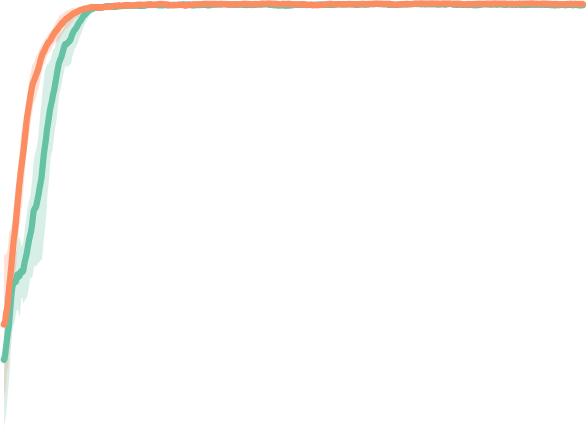
\includegraphics[interpolate=true,width=2.000000in,height=2.140000in]{shape-10-img1.png}}%
\end{pgfscope}%
\begin{pgfscope}%
\pgfsetrectcap%
\pgfsetmiterjoin%
\pgfsetlinewidth{0.803000pt}%
\definecolor{currentstroke}{rgb}{0.000000,0.000000,0.000000}%
\pgfsetstrokecolor{currentstroke}%
\pgfsetdash{}{0pt}%
\pgfpathmoveto{\pgfqpoint{0.602198in}{0.524170in}}%
\pgfpathlineto{\pgfqpoint{0.602198in}{3.041514in}}%
\pgfusepath{stroke}%
\end{pgfscope}%
\begin{pgfscope}%
\pgfsetrectcap%
\pgfsetmiterjoin%
\pgfsetlinewidth{0.803000pt}%
\definecolor{currentstroke}{rgb}{0.000000,0.000000,0.000000}%
\pgfsetstrokecolor{currentstroke}%
\pgfsetdash{}{0pt}%
\pgfpathmoveto{\pgfqpoint{2.760816in}{0.524170in}}%
\pgfpathlineto{\pgfqpoint{2.760816in}{3.041514in}}%
\pgfusepath{stroke}%
\end{pgfscope}%
\begin{pgfscope}%
\pgfsetrectcap%
\pgfsetmiterjoin%
\pgfsetlinewidth{0.803000pt}%
\definecolor{currentstroke}{rgb}{0.000000,0.000000,0.000000}%
\pgfsetstrokecolor{currentstroke}%
\pgfsetdash{}{0pt}%
\pgfpathmoveto{\pgfqpoint{0.602198in}{0.524170in}}%
\pgfpathlineto{\pgfqpoint{2.760816in}{0.524170in}}%
\pgfusepath{stroke}%
\end{pgfscope}%
\begin{pgfscope}%
\pgfsetrectcap%
\pgfsetmiterjoin%
\pgfsetlinewidth{0.803000pt}%
\definecolor{currentstroke}{rgb}{0.000000,0.000000,0.000000}%
\pgfsetstrokecolor{currentstroke}%
\pgfsetdash{}{0pt}%
\pgfpathmoveto{\pgfqpoint{0.602198in}{3.041514in}}%
\pgfpathlineto{\pgfqpoint{2.760816in}{3.041514in}}%
\pgfusepath{stroke}%
\end{pgfscope}%
\begin{pgfscope}%
\pgfsetrectcap%
\pgfsetroundjoin%
\pgfsetlinewidth{1.505625pt}%
\definecolor{currentstroke}{rgb}{0.000000,0.419608,0.643137}%
\pgfsetstrokecolor{currentstroke}%
\pgfsetdash{}{0pt}%
\pgfpathmoveto{\pgfqpoint{2.011923in}{1.872621in}}%
\pgfpathlineto{\pgfqpoint{2.123034in}{1.872621in}}%
\pgfpathlineto{\pgfqpoint{2.234146in}{1.872621in}}%
\pgfusepath{stroke}%
\end{pgfscope}%
\begin{pgfscope}%
\definecolor{textcolor}{rgb}{0.000000,0.000000,0.000000}%
\pgfsetstrokecolor{textcolor}%
\pgfsetfillcolor{textcolor}%
\pgftext[x=2.323034in,y=1.833732in,left,base]{\color{textcolor}\rmfamily\fontsize{8.000000}{9.600000}\selectfont LSTM}%
\end{pgfscope}%
\begin{pgfscope}%
\pgfsetrectcap%
\pgfsetroundjoin%
\pgfsetlinewidth{1.505625pt}%
\definecolor{currentstroke}{rgb}{1.000000,0.501961,0.054902}%
\pgfsetstrokecolor{currentstroke}%
\pgfsetdash{}{0pt}%
\pgfpathmoveto{\pgfqpoint{2.011923in}{1.709535in}}%
\pgfpathlineto{\pgfqpoint{2.123034in}{1.709535in}}%
\pgfpathlineto{\pgfqpoint{2.234146in}{1.709535in}}%
\pgfusepath{stroke}%
\end{pgfscope}%
\begin{pgfscope}%
\definecolor{textcolor}{rgb}{0.000000,0.000000,0.000000}%
\pgfsetstrokecolor{textcolor}%
\pgfsetfillcolor{textcolor}%
\pgftext[x=2.323034in,y=1.670646in,left,base]{\color{textcolor}\rmfamily\fontsize{8.000000}{9.600000}\selectfont MAP}%
\end{pgfscope}%
\begin{pgfscope}%
\pgfsetbuttcap%
\pgfsetmiterjoin%
\definecolor{currentfill}{rgb}{1.000000,1.000000,1.000000}%
\pgfsetfillcolor{currentfill}%
\pgfsetlinewidth{0.000000pt}%
\definecolor{currentstroke}{rgb}{0.000000,0.000000,0.000000}%
\pgfsetstrokecolor{currentstroke}%
\pgfsetstrokeopacity{0.000000}%
\pgfsetdash{}{0pt}%
\pgfpathmoveto{\pgfqpoint{3.336877in}{0.524170in}}%
\pgfpathlineto{\pgfqpoint{5.495496in}{0.524170in}}%
\pgfpathlineto{\pgfqpoint{5.495496in}{3.041514in}}%
\pgfpathlineto{\pgfqpoint{3.336877in}{3.041514in}}%
\pgfpathlineto{\pgfqpoint{3.336877in}{0.524170in}}%
\pgfpathclose%
\pgfusepath{fill}%
\end{pgfscope}%
\begin{pgfscope}%
\pgfsys@transformshift{3.440000in}{0.639108in}%
\pgftext[left,bottom]{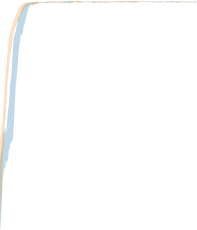
\includegraphics[interpolate=true,width=1.970000in,height=2.300000in]{shape-10-img2.png}}%
\end{pgfscope}%
\begin{pgfscope}%
\pgfsetbuttcap%
\pgfsetroundjoin%
\definecolor{currentfill}{rgb}{0.000000,0.000000,0.000000}%
\pgfsetfillcolor{currentfill}%
\pgfsetlinewidth{0.803000pt}%
\definecolor{currentstroke}{rgb}{0.000000,0.000000,0.000000}%
\pgfsetstrokecolor{currentstroke}%
\pgfsetdash{}{0pt}%
\pgfsys@defobject{currentmarker}{\pgfqpoint{0.000000in}{-0.048611in}}{\pgfqpoint{0.000000in}{0.000000in}}{%
\pgfpathmoveto{\pgfqpoint{0.000000in}{0.000000in}}%
\pgfpathlineto{\pgfqpoint{0.000000in}{-0.048611in}}%
\pgfusepath{stroke,fill}%
}%
\begin{pgfscope}%
\pgfsys@transformshift{3.408883in}{0.524170in}%
\pgfsys@useobject{currentmarker}{}%
\end{pgfscope}%
\end{pgfscope}%
\begin{pgfscope}%
\definecolor{textcolor}{rgb}{0.000000,0.000000,0.000000}%
\pgfsetstrokecolor{textcolor}%
\pgfsetfillcolor{textcolor}%
\pgftext[x=3.408883in,y=0.426948in,,top]{\color{textcolor}\rmfamily\fontsize{8.000000}{9.600000}\selectfont \(\displaystyle {0.0}\)}%
\end{pgfscope}%
\begin{pgfscope}%
\pgfsetbuttcap%
\pgfsetroundjoin%
\definecolor{currentfill}{rgb}{0.000000,0.000000,0.000000}%
\pgfsetfillcolor{currentfill}%
\pgfsetlinewidth{0.803000pt}%
\definecolor{currentstroke}{rgb}{0.000000,0.000000,0.000000}%
\pgfsetstrokecolor{currentstroke}%
\pgfsetdash{}{0pt}%
\pgfsys@defobject{currentmarker}{\pgfqpoint{0.000000in}{-0.048611in}}{\pgfqpoint{0.000000in}{0.000000in}}{%
\pgfpathmoveto{\pgfqpoint{0.000000in}{0.000000in}}%
\pgfpathlineto{\pgfqpoint{0.000000in}{-0.048611in}}%
\pgfusepath{stroke,fill}%
}%
\begin{pgfscope}%
\pgfsys@transformshift{3.806843in}{0.524170in}%
\pgfsys@useobject{currentmarker}{}%
\end{pgfscope}%
\end{pgfscope}%
\begin{pgfscope}%
\definecolor{textcolor}{rgb}{0.000000,0.000000,0.000000}%
\pgfsetstrokecolor{textcolor}%
\pgfsetfillcolor{textcolor}%
\pgftext[x=3.806843in,y=0.426948in,,top]{\color{textcolor}\rmfamily\fontsize{8.000000}{9.600000}\selectfont \(\displaystyle {0.5}\)}%
\end{pgfscope}%
\begin{pgfscope}%
\pgfsetbuttcap%
\pgfsetroundjoin%
\definecolor{currentfill}{rgb}{0.000000,0.000000,0.000000}%
\pgfsetfillcolor{currentfill}%
\pgfsetlinewidth{0.803000pt}%
\definecolor{currentstroke}{rgb}{0.000000,0.000000,0.000000}%
\pgfsetstrokecolor{currentstroke}%
\pgfsetdash{}{0pt}%
\pgfsys@defobject{currentmarker}{\pgfqpoint{0.000000in}{-0.048611in}}{\pgfqpoint{0.000000in}{0.000000in}}{%
\pgfpathmoveto{\pgfqpoint{0.000000in}{0.000000in}}%
\pgfpathlineto{\pgfqpoint{0.000000in}{-0.048611in}}%
\pgfusepath{stroke,fill}%
}%
\begin{pgfscope}%
\pgfsys@transformshift{4.204803in}{0.524170in}%
\pgfsys@useobject{currentmarker}{}%
\end{pgfscope}%
\end{pgfscope}%
\begin{pgfscope}%
\definecolor{textcolor}{rgb}{0.000000,0.000000,0.000000}%
\pgfsetstrokecolor{textcolor}%
\pgfsetfillcolor{textcolor}%
\pgftext[x=4.204803in,y=0.426948in,,top]{\color{textcolor}\rmfamily\fontsize{8.000000}{9.600000}\selectfont \(\displaystyle {1.0}\)}%
\end{pgfscope}%
\begin{pgfscope}%
\pgfsetbuttcap%
\pgfsetroundjoin%
\definecolor{currentfill}{rgb}{0.000000,0.000000,0.000000}%
\pgfsetfillcolor{currentfill}%
\pgfsetlinewidth{0.803000pt}%
\definecolor{currentstroke}{rgb}{0.000000,0.000000,0.000000}%
\pgfsetstrokecolor{currentstroke}%
\pgfsetdash{}{0pt}%
\pgfsys@defobject{currentmarker}{\pgfqpoint{0.000000in}{-0.048611in}}{\pgfqpoint{0.000000in}{0.000000in}}{%
\pgfpathmoveto{\pgfqpoint{0.000000in}{0.000000in}}%
\pgfpathlineto{\pgfqpoint{0.000000in}{-0.048611in}}%
\pgfusepath{stroke,fill}%
}%
\begin{pgfscope}%
\pgfsys@transformshift{4.602763in}{0.524170in}%
\pgfsys@useobject{currentmarker}{}%
\end{pgfscope}%
\end{pgfscope}%
\begin{pgfscope}%
\definecolor{textcolor}{rgb}{0.000000,0.000000,0.000000}%
\pgfsetstrokecolor{textcolor}%
\pgfsetfillcolor{textcolor}%
\pgftext[x=4.602763in,y=0.426948in,,top]{\color{textcolor}\rmfamily\fontsize{8.000000}{9.600000}\selectfont \(\displaystyle {1.5}\)}%
\end{pgfscope}%
\begin{pgfscope}%
\pgfsetbuttcap%
\pgfsetroundjoin%
\definecolor{currentfill}{rgb}{0.000000,0.000000,0.000000}%
\pgfsetfillcolor{currentfill}%
\pgfsetlinewidth{0.803000pt}%
\definecolor{currentstroke}{rgb}{0.000000,0.000000,0.000000}%
\pgfsetstrokecolor{currentstroke}%
\pgfsetdash{}{0pt}%
\pgfsys@defobject{currentmarker}{\pgfqpoint{0.000000in}{-0.048611in}}{\pgfqpoint{0.000000in}{0.000000in}}{%
\pgfpathmoveto{\pgfqpoint{0.000000in}{0.000000in}}%
\pgfpathlineto{\pgfqpoint{0.000000in}{-0.048611in}}%
\pgfusepath{stroke,fill}%
}%
\begin{pgfscope}%
\pgfsys@transformshift{5.000723in}{0.524170in}%
\pgfsys@useobject{currentmarker}{}%
\end{pgfscope}%
\end{pgfscope}%
\begin{pgfscope}%
\definecolor{textcolor}{rgb}{0.000000,0.000000,0.000000}%
\pgfsetstrokecolor{textcolor}%
\pgfsetfillcolor{textcolor}%
\pgftext[x=5.000723in,y=0.426948in,,top]{\color{textcolor}\rmfamily\fontsize{8.000000}{9.600000}\selectfont \(\displaystyle {2.0}\)}%
\end{pgfscope}%
\begin{pgfscope}%
\pgfsetbuttcap%
\pgfsetroundjoin%
\definecolor{currentfill}{rgb}{0.000000,0.000000,0.000000}%
\pgfsetfillcolor{currentfill}%
\pgfsetlinewidth{0.803000pt}%
\definecolor{currentstroke}{rgb}{0.000000,0.000000,0.000000}%
\pgfsetstrokecolor{currentstroke}%
\pgfsetdash{}{0pt}%
\pgfsys@defobject{currentmarker}{\pgfqpoint{0.000000in}{-0.048611in}}{\pgfqpoint{0.000000in}{0.000000in}}{%
\pgfpathmoveto{\pgfqpoint{0.000000in}{0.000000in}}%
\pgfpathlineto{\pgfqpoint{0.000000in}{-0.048611in}}%
\pgfusepath{stroke,fill}%
}%
\begin{pgfscope}%
\pgfsys@transformshift{5.398683in}{0.524170in}%
\pgfsys@useobject{currentmarker}{}%
\end{pgfscope}%
\end{pgfscope}%
\begin{pgfscope}%
\definecolor{textcolor}{rgb}{0.000000,0.000000,0.000000}%
\pgfsetstrokecolor{textcolor}%
\pgfsetfillcolor{textcolor}%
\pgftext[x=5.398683in,y=0.426948in,,top]{\color{textcolor}\rmfamily\fontsize{8.000000}{9.600000}\selectfont \(\displaystyle {2.5}\)}%
\end{pgfscope}%
\begin{pgfscope}%
\definecolor{textcolor}{rgb}{0.000000,0.000000,0.000000}%
\pgfsetstrokecolor{textcolor}%
\pgfsetfillcolor{textcolor}%
\pgftext[x=4.416187in,y=0.263862in,,top]{\color{textcolor}\rmfamily\fontsize{10.000000}{12.000000}\selectfont step}%
\end{pgfscope}%
\begin{pgfscope}%
\definecolor{textcolor}{rgb}{0.000000,0.000000,0.000000}%
\pgfsetstrokecolor{textcolor}%
\pgfsetfillcolor{textcolor}%
\pgftext[x=5.495496in,y=0.277751in,right,top]{\color{textcolor}\rmfamily\fontsize{8.000000}{9.600000}\selectfont \(\displaystyle \times{10^{7}}{}\)}%
\end{pgfscope}%
\begin{pgfscope}%
\pgfsetbuttcap%
\pgfsetroundjoin%
\definecolor{currentfill}{rgb}{0.000000,0.000000,0.000000}%
\pgfsetfillcolor{currentfill}%
\pgfsetlinewidth{0.803000pt}%
\definecolor{currentstroke}{rgb}{0.000000,0.000000,0.000000}%
\pgfsetstrokecolor{currentstroke}%
\pgfsetdash{}{0pt}%
\pgfsys@defobject{currentmarker}{\pgfqpoint{-0.048611in}{0.000000in}}{\pgfqpoint{-0.000000in}{0.000000in}}{%
\pgfpathmoveto{\pgfqpoint{-0.000000in}{0.000000in}}%
\pgfpathlineto{\pgfqpoint{-0.048611in}{0.000000in}}%
\pgfusepath{stroke,fill}%
}%
\begin{pgfscope}%
\pgfsys@transformshift{3.336877in}{0.813129in}%
\pgfsys@useobject{currentmarker}{}%
\end{pgfscope}%
\end{pgfscope}%
\begin{pgfscope}%
\definecolor{textcolor}{rgb}{0.000000,0.000000,0.000000}%
\pgfsetstrokecolor{textcolor}%
\pgfsetfillcolor{textcolor}%
\pgftext[x=3.088804in, y=0.770920in, left, base]{\color{textcolor}\rmfamily\fontsize{8.000000}{9.600000}\selectfont \(\displaystyle {0.5}\)}%
\end{pgfscope}%
\begin{pgfscope}%
\pgfsetbuttcap%
\pgfsetroundjoin%
\definecolor{currentfill}{rgb}{0.000000,0.000000,0.000000}%
\pgfsetfillcolor{currentfill}%
\pgfsetlinewidth{0.803000pt}%
\definecolor{currentstroke}{rgb}{0.000000,0.000000,0.000000}%
\pgfsetstrokecolor{currentstroke}%
\pgfsetdash{}{0pt}%
\pgfsys@defobject{currentmarker}{\pgfqpoint{-0.048611in}{0.000000in}}{\pgfqpoint{-0.000000in}{0.000000in}}{%
\pgfpathmoveto{\pgfqpoint{-0.000000in}{0.000000in}}%
\pgfpathlineto{\pgfqpoint{-0.048611in}{0.000000in}}%
\pgfusepath{stroke,fill}%
}%
\begin{pgfscope}%
\pgfsys@transformshift{3.336877in}{1.235575in}%
\pgfsys@useobject{currentmarker}{}%
\end{pgfscope}%
\end{pgfscope}%
\begin{pgfscope}%
\definecolor{textcolor}{rgb}{0.000000,0.000000,0.000000}%
\pgfsetstrokecolor{textcolor}%
\pgfsetfillcolor{textcolor}%
\pgftext[x=3.088804in, y=1.193366in, left, base]{\color{textcolor}\rmfamily\fontsize{8.000000}{9.600000}\selectfont \(\displaystyle {0.6}\)}%
\end{pgfscope}%
\begin{pgfscope}%
\pgfsetbuttcap%
\pgfsetroundjoin%
\definecolor{currentfill}{rgb}{0.000000,0.000000,0.000000}%
\pgfsetfillcolor{currentfill}%
\pgfsetlinewidth{0.803000pt}%
\definecolor{currentstroke}{rgb}{0.000000,0.000000,0.000000}%
\pgfsetstrokecolor{currentstroke}%
\pgfsetdash{}{0pt}%
\pgfsys@defobject{currentmarker}{\pgfqpoint{-0.048611in}{0.000000in}}{\pgfqpoint{-0.000000in}{0.000000in}}{%
\pgfpathmoveto{\pgfqpoint{-0.000000in}{0.000000in}}%
\pgfpathlineto{\pgfqpoint{-0.048611in}{0.000000in}}%
\pgfusepath{stroke,fill}%
}%
\begin{pgfscope}%
\pgfsys@transformshift{3.336877in}{1.658021in}%
\pgfsys@useobject{currentmarker}{}%
\end{pgfscope}%
\end{pgfscope}%
\begin{pgfscope}%
\definecolor{textcolor}{rgb}{0.000000,0.000000,0.000000}%
\pgfsetstrokecolor{textcolor}%
\pgfsetfillcolor{textcolor}%
\pgftext[x=3.088804in, y=1.615812in, left, base]{\color{textcolor}\rmfamily\fontsize{8.000000}{9.600000}\selectfont \(\displaystyle {0.7}\)}%
\end{pgfscope}%
\begin{pgfscope}%
\pgfsetbuttcap%
\pgfsetroundjoin%
\definecolor{currentfill}{rgb}{0.000000,0.000000,0.000000}%
\pgfsetfillcolor{currentfill}%
\pgfsetlinewidth{0.803000pt}%
\definecolor{currentstroke}{rgb}{0.000000,0.000000,0.000000}%
\pgfsetstrokecolor{currentstroke}%
\pgfsetdash{}{0pt}%
\pgfsys@defobject{currentmarker}{\pgfqpoint{-0.048611in}{0.000000in}}{\pgfqpoint{-0.000000in}{0.000000in}}{%
\pgfpathmoveto{\pgfqpoint{-0.000000in}{0.000000in}}%
\pgfpathlineto{\pgfqpoint{-0.048611in}{0.000000in}}%
\pgfusepath{stroke,fill}%
}%
\begin{pgfscope}%
\pgfsys@transformshift{3.336877in}{2.080467in}%
\pgfsys@useobject{currentmarker}{}%
\end{pgfscope}%
\end{pgfscope}%
\begin{pgfscope}%
\definecolor{textcolor}{rgb}{0.000000,0.000000,0.000000}%
\pgfsetstrokecolor{textcolor}%
\pgfsetfillcolor{textcolor}%
\pgftext[x=3.088804in, y=2.038257in, left, base]{\color{textcolor}\rmfamily\fontsize{8.000000}{9.600000}\selectfont \(\displaystyle {0.8}\)}%
\end{pgfscope}%
\begin{pgfscope}%
\pgfsetbuttcap%
\pgfsetroundjoin%
\definecolor{currentfill}{rgb}{0.000000,0.000000,0.000000}%
\pgfsetfillcolor{currentfill}%
\pgfsetlinewidth{0.803000pt}%
\definecolor{currentstroke}{rgb}{0.000000,0.000000,0.000000}%
\pgfsetstrokecolor{currentstroke}%
\pgfsetdash{}{0pt}%
\pgfsys@defobject{currentmarker}{\pgfqpoint{-0.048611in}{0.000000in}}{\pgfqpoint{-0.000000in}{0.000000in}}{%
\pgfpathmoveto{\pgfqpoint{-0.000000in}{0.000000in}}%
\pgfpathlineto{\pgfqpoint{-0.048611in}{0.000000in}}%
\pgfusepath{stroke,fill}%
}%
\begin{pgfscope}%
\pgfsys@transformshift{3.336877in}{2.502912in}%
\pgfsys@useobject{currentmarker}{}%
\end{pgfscope}%
\end{pgfscope}%
\begin{pgfscope}%
\definecolor{textcolor}{rgb}{0.000000,0.000000,0.000000}%
\pgfsetstrokecolor{textcolor}%
\pgfsetfillcolor{textcolor}%
\pgftext[x=3.088804in, y=2.460703in, left, base]{\color{textcolor}\rmfamily\fontsize{8.000000}{9.600000}\selectfont \(\displaystyle {0.9}\)}%
\end{pgfscope}%
\begin{pgfscope}%
\pgfsetbuttcap%
\pgfsetroundjoin%
\definecolor{currentfill}{rgb}{0.000000,0.000000,0.000000}%
\pgfsetfillcolor{currentfill}%
\pgfsetlinewidth{0.803000pt}%
\definecolor{currentstroke}{rgb}{0.000000,0.000000,0.000000}%
\pgfsetstrokecolor{currentstroke}%
\pgfsetdash{}{0pt}%
\pgfsys@defobject{currentmarker}{\pgfqpoint{-0.048611in}{0.000000in}}{\pgfqpoint{-0.000000in}{0.000000in}}{%
\pgfpathmoveto{\pgfqpoint{-0.000000in}{0.000000in}}%
\pgfpathlineto{\pgfqpoint{-0.048611in}{0.000000in}}%
\pgfusepath{stroke,fill}%
}%
\begin{pgfscope}%
\pgfsys@transformshift{3.336877in}{2.925358in}%
\pgfsys@useobject{currentmarker}{}%
\end{pgfscope}%
\end{pgfscope}%
\begin{pgfscope}%
\definecolor{textcolor}{rgb}{0.000000,0.000000,0.000000}%
\pgfsetstrokecolor{textcolor}%
\pgfsetfillcolor{textcolor}%
\pgftext[x=3.088804in, y=2.883149in, left, base]{\color{textcolor}\rmfamily\fontsize{8.000000}{9.600000}\selectfont \(\displaystyle {1.0}\)}%
\end{pgfscope}%
\begin{pgfscope}%
\definecolor{textcolor}{rgb}{0.000000,0.000000,0.000000}%
\pgfsetstrokecolor{textcolor}%
\pgfsetfillcolor{textcolor}%
\pgftext[x=3.033248in,y=1.782842in,,bottom,rotate=90.000000]{\color{textcolor}\rmfamily\fontsize{10.000000}{12.000000}\selectfont success}%
\end{pgfscope}%
\begin{pgfscope}%
\pgfsys@transformshift{3.420000in}{0.989108in}%
\pgftext[left,bottom]{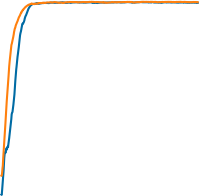
\includegraphics[interpolate=true,width=2.000000in,height=1.960000in]{shape-10-img3.png}}%
\end{pgfscope}%
\begin{pgfscope}%
\pgfsetrectcap%
\pgfsetmiterjoin%
\pgfsetlinewidth{0.803000pt}%
\definecolor{currentstroke}{rgb}{0.000000,0.000000,0.000000}%
\pgfsetstrokecolor{currentstroke}%
\pgfsetdash{}{0pt}%
\pgfpathmoveto{\pgfqpoint{3.336877in}{0.524170in}}%
\pgfpathlineto{\pgfqpoint{3.336877in}{3.041514in}}%
\pgfusepath{stroke}%
\end{pgfscope}%
\begin{pgfscope}%
\pgfsetrectcap%
\pgfsetmiterjoin%
\pgfsetlinewidth{0.803000pt}%
\definecolor{currentstroke}{rgb}{0.000000,0.000000,0.000000}%
\pgfsetstrokecolor{currentstroke}%
\pgfsetdash{}{0pt}%
\pgfpathmoveto{\pgfqpoint{5.495496in}{0.524170in}}%
\pgfpathlineto{\pgfqpoint{5.495496in}{3.041514in}}%
\pgfusepath{stroke}%
\end{pgfscope}%
\begin{pgfscope}%
\pgfsetrectcap%
\pgfsetmiterjoin%
\pgfsetlinewidth{0.803000pt}%
\definecolor{currentstroke}{rgb}{0.000000,0.000000,0.000000}%
\pgfsetstrokecolor{currentstroke}%
\pgfsetdash{}{0pt}%
\pgfpathmoveto{\pgfqpoint{3.336877in}{0.524170in}}%
\pgfpathlineto{\pgfqpoint{5.495496in}{0.524170in}}%
\pgfusepath{stroke}%
\end{pgfscope}%
\begin{pgfscope}%
\pgfsetrectcap%
\pgfsetmiterjoin%
\pgfsetlinewidth{0.803000pt}%
\definecolor{currentstroke}{rgb}{0.000000,0.000000,0.000000}%
\pgfsetstrokecolor{currentstroke}%
\pgfsetdash{}{0pt}%
\pgfpathmoveto{\pgfqpoint{3.336877in}{3.041514in}}%
\pgfpathlineto{\pgfqpoint{5.495496in}{3.041514in}}%
\pgfusepath{stroke}%
\end{pgfscope}%
\begin{pgfscope}%
\pgfsetrectcap%
\pgfsetroundjoin%
\pgfsetlinewidth{1.505625pt}%
\definecolor{currentstroke}{rgb}{0.000000,0.419608,0.643137}%
\pgfsetstrokecolor{currentstroke}%
\pgfsetdash{}{0pt}%
\pgfpathmoveto{\pgfqpoint{4.746603in}{1.872621in}}%
\pgfpathlineto{\pgfqpoint{4.857714in}{1.872621in}}%
\pgfpathlineto{\pgfqpoint{4.968825in}{1.872621in}}%
\pgfusepath{stroke}%
\end{pgfscope}%
\begin{pgfscope}%
\definecolor{textcolor}{rgb}{0.000000,0.000000,0.000000}%
\pgfsetstrokecolor{textcolor}%
\pgfsetfillcolor{textcolor}%
\pgftext[x=5.057714in,y=1.833732in,left,base]{\color{textcolor}\rmfamily\fontsize{8.000000}{9.600000}\selectfont LSTM}%
\end{pgfscope}%
\begin{pgfscope}%
\pgfsetrectcap%
\pgfsetroundjoin%
\pgfsetlinewidth{1.505625pt}%
\definecolor{currentstroke}{rgb}{1.000000,0.501961,0.054902}%
\pgfsetstrokecolor{currentstroke}%
\pgfsetdash{}{0pt}%
\pgfpathmoveto{\pgfqpoint{4.746603in}{1.709535in}}%
\pgfpathlineto{\pgfqpoint{4.857714in}{1.709535in}}%
\pgfpathlineto{\pgfqpoint{4.968825in}{1.709535in}}%
\pgfusepath{stroke}%
\end{pgfscope}%
\begin{pgfscope}%
\definecolor{textcolor}{rgb}{0.000000,0.000000,0.000000}%
\pgfsetstrokecolor{textcolor}%
\pgfsetfillcolor{textcolor}%
\pgftext[x=5.057714in,y=1.670646in,left,base]{\color{textcolor}\rmfamily\fontsize{8.000000}{9.600000}\selectfont MAP}%
\end{pgfscope}%
\begin{pgfscope}%
\definecolor{textcolor}{rgb}{0.000000,0.000000,0.000000}%
\pgfsetstrokecolor{textcolor}%
\pgfsetfillcolor{textcolor}%
\pgftext[x=2.822748in,y=3.419326in,,top]{\color{textcolor}\rmfamily\fontsize{12.000000}{14.400000}\selectfont \(\displaystyle 10 \times 10\) search space}%
\end{pgfscope}%
\end{pgfpicture}%
\makeatother%
\endgroup%

    \(15 \times 15\)
    %% Creator: Matplotlib, PGF backend
%%
%% To include the figure in your LaTeX document, write
%%   \input{<filename>.pgf}
%%
%% Make sure the required packages are loaded in your preamble
%%   \usepackage{pgf}
%%
%% Also ensure that all the required font packages are loaded; for instance,
%% the lmodern package is sometimes necessary when using math font.
%%   \usepackage{lmodern}
%%
%% Figures using additional raster images can only be included by \input if
%% they are in the same directory as the main LaTeX file. For loading figures
%% from other directories you can use the `import` package
%%   \usepackage{import}
%%
%% and then include the figures with
%%   \import{<path to file>}{<filename>.pgf}
%%
%% Matplotlib used the following preamble
%%   \usepackage{fontspec}
%%   \setmainfont{DejaVuSerif.ttf}[Path=\detokenize{/home/oslund/.local/lib/python3.8/site-packages/matplotlib/mpl-data/fonts/ttf/}]
%%   \setsansfont{DejaVuSans.ttf}[Path=\detokenize{/home/oslund/.local/lib/python3.8/site-packages/matplotlib/mpl-data/fonts/ttf/}]
%%   \setmonofont{DejaVuSansMono.ttf}[Path=\detokenize{/home/oslund/.local/lib/python3.8/site-packages/matplotlib/mpl-data/fonts/ttf/}]
%%
\begingroup%
\makeatletter%
\begin{pgfpicture}%
\pgfpathrectangle{\pgfpointorigin}{\pgfqpoint{5.645496in}{2.258198in}}%
\pgfusepath{use as bounding box, clip}%
\begin{pgfscope}%
\pgfsetbuttcap%
\pgfsetmiterjoin%
\definecolor{currentfill}{rgb}{1.000000,1.000000,1.000000}%
\pgfsetfillcolor{currentfill}%
\pgfsetlinewidth{0.000000pt}%
\definecolor{currentstroke}{rgb}{1.000000,1.000000,1.000000}%
\pgfsetstrokecolor{currentstroke}%
\pgfsetdash{}{0pt}%
\pgfpathmoveto{\pgfqpoint{0.000000in}{0.000000in}}%
\pgfpathlineto{\pgfqpoint{5.645496in}{0.000000in}}%
\pgfpathlineto{\pgfqpoint{5.645496in}{2.258198in}}%
\pgfpathlineto{\pgfqpoint{0.000000in}{2.258198in}}%
\pgfpathlineto{\pgfqpoint{0.000000in}{0.000000in}}%
\pgfpathclose%
\pgfusepath{fill}%
\end{pgfscope}%
\begin{pgfscope}%
\pgfsetbuttcap%
\pgfsetmiterjoin%
\definecolor{currentfill}{rgb}{1.000000,1.000000,1.000000}%
\pgfsetfillcolor{currentfill}%
\pgfsetlinewidth{0.000000pt}%
\definecolor{currentstroke}{rgb}{0.000000,0.000000,0.000000}%
\pgfsetstrokecolor{currentstroke}%
\pgfsetstrokeopacity{0.000000}%
\pgfsetdash{}{0pt}%
\pgfpathmoveto{\pgfqpoint{0.695728in}{0.558892in}}%
\pgfpathlineto{\pgfqpoint{2.790221in}{0.558892in}}%
\pgfpathlineto{\pgfqpoint{2.790221in}{2.098138in}}%
\pgfpathlineto{\pgfqpoint{0.695728in}{2.098138in}}%
\pgfpathlineto{\pgfqpoint{0.695728in}{0.558892in}}%
\pgfpathclose%
\pgfusepath{fill}%
\end{pgfscope}%
\begin{pgfscope}%
\pgfsetbuttcap%
\pgfsetroundjoin%
\definecolor{currentfill}{rgb}{0.150000,0.150000,0.150000}%
\pgfsetfillcolor{currentfill}%
\pgfsetlinewidth{1.254687pt}%
\definecolor{currentstroke}{rgb}{0.150000,0.150000,0.150000}%
\pgfsetstrokecolor{currentstroke}%
\pgfsetdash{}{0pt}%
\pgfsys@defobject{currentmarker}{\pgfqpoint{0.000000in}{-0.083333in}}{\pgfqpoint{0.000000in}{0.000000in}}{%
\pgfpathmoveto{\pgfqpoint{0.000000in}{0.000000in}}%
\pgfpathlineto{\pgfqpoint{0.000000in}{-0.083333in}}%
\pgfusepath{stroke,fill}%
}%
\begin{pgfscope}%
\pgfsys@transformshift{0.765595in}{0.558892in}%
\pgfsys@useobject{currentmarker}{}%
\end{pgfscope}%
\end{pgfscope}%
\begin{pgfscope}%
\definecolor{textcolor}{rgb}{0.150000,0.150000,0.150000}%
\pgfsetstrokecolor{textcolor}%
\pgfsetfillcolor{textcolor}%
\pgftext[x=0.765595in,y=0.426948in,,top]{\color{textcolor}\rmfamily\fontsize{8.000000}{9.600000}\selectfont \(\displaystyle {0.0}\)}%
\end{pgfscope}%
\begin{pgfscope}%
\pgfsetbuttcap%
\pgfsetroundjoin%
\definecolor{currentfill}{rgb}{0.150000,0.150000,0.150000}%
\pgfsetfillcolor{currentfill}%
\pgfsetlinewidth{1.254687pt}%
\definecolor{currentstroke}{rgb}{0.150000,0.150000,0.150000}%
\pgfsetstrokecolor{currentstroke}%
\pgfsetdash{}{0pt}%
\pgfsys@defobject{currentmarker}{\pgfqpoint{0.000000in}{-0.083333in}}{\pgfqpoint{0.000000in}{0.000000in}}{%
\pgfpathmoveto{\pgfqpoint{0.000000in}{0.000000in}}%
\pgfpathlineto{\pgfqpoint{0.000000in}{-0.083333in}}%
\pgfusepath{stroke,fill}%
}%
\begin{pgfscope}%
\pgfsys@transformshift{1.151733in}{0.558892in}%
\pgfsys@useobject{currentmarker}{}%
\end{pgfscope}%
\end{pgfscope}%
\begin{pgfscope}%
\definecolor{textcolor}{rgb}{0.150000,0.150000,0.150000}%
\pgfsetstrokecolor{textcolor}%
\pgfsetfillcolor{textcolor}%
\pgftext[x=1.151733in,y=0.426948in,,top]{\color{textcolor}\rmfamily\fontsize{8.000000}{9.600000}\selectfont \(\displaystyle {0.5}\)}%
\end{pgfscope}%
\begin{pgfscope}%
\pgfsetbuttcap%
\pgfsetroundjoin%
\definecolor{currentfill}{rgb}{0.150000,0.150000,0.150000}%
\pgfsetfillcolor{currentfill}%
\pgfsetlinewidth{1.254687pt}%
\definecolor{currentstroke}{rgb}{0.150000,0.150000,0.150000}%
\pgfsetstrokecolor{currentstroke}%
\pgfsetdash{}{0pt}%
\pgfsys@defobject{currentmarker}{\pgfqpoint{0.000000in}{-0.083333in}}{\pgfqpoint{0.000000in}{0.000000in}}{%
\pgfpathmoveto{\pgfqpoint{0.000000in}{0.000000in}}%
\pgfpathlineto{\pgfqpoint{0.000000in}{-0.083333in}}%
\pgfusepath{stroke,fill}%
}%
\begin{pgfscope}%
\pgfsys@transformshift{1.537870in}{0.558892in}%
\pgfsys@useobject{currentmarker}{}%
\end{pgfscope}%
\end{pgfscope}%
\begin{pgfscope}%
\definecolor{textcolor}{rgb}{0.150000,0.150000,0.150000}%
\pgfsetstrokecolor{textcolor}%
\pgfsetfillcolor{textcolor}%
\pgftext[x=1.537870in,y=0.426948in,,top]{\color{textcolor}\rmfamily\fontsize{8.000000}{9.600000}\selectfont \(\displaystyle {1.0}\)}%
\end{pgfscope}%
\begin{pgfscope}%
\pgfsetbuttcap%
\pgfsetroundjoin%
\definecolor{currentfill}{rgb}{0.150000,0.150000,0.150000}%
\pgfsetfillcolor{currentfill}%
\pgfsetlinewidth{1.254687pt}%
\definecolor{currentstroke}{rgb}{0.150000,0.150000,0.150000}%
\pgfsetstrokecolor{currentstroke}%
\pgfsetdash{}{0pt}%
\pgfsys@defobject{currentmarker}{\pgfqpoint{0.000000in}{-0.083333in}}{\pgfqpoint{0.000000in}{0.000000in}}{%
\pgfpathmoveto{\pgfqpoint{0.000000in}{0.000000in}}%
\pgfpathlineto{\pgfqpoint{0.000000in}{-0.083333in}}%
\pgfusepath{stroke,fill}%
}%
\begin{pgfscope}%
\pgfsys@transformshift{1.924008in}{0.558892in}%
\pgfsys@useobject{currentmarker}{}%
\end{pgfscope}%
\end{pgfscope}%
\begin{pgfscope}%
\definecolor{textcolor}{rgb}{0.150000,0.150000,0.150000}%
\pgfsetstrokecolor{textcolor}%
\pgfsetfillcolor{textcolor}%
\pgftext[x=1.924008in,y=0.426948in,,top]{\color{textcolor}\rmfamily\fontsize{8.000000}{9.600000}\selectfont \(\displaystyle {1.5}\)}%
\end{pgfscope}%
\begin{pgfscope}%
\pgfsetbuttcap%
\pgfsetroundjoin%
\definecolor{currentfill}{rgb}{0.150000,0.150000,0.150000}%
\pgfsetfillcolor{currentfill}%
\pgfsetlinewidth{1.254687pt}%
\definecolor{currentstroke}{rgb}{0.150000,0.150000,0.150000}%
\pgfsetstrokecolor{currentstroke}%
\pgfsetdash{}{0pt}%
\pgfsys@defobject{currentmarker}{\pgfqpoint{0.000000in}{-0.083333in}}{\pgfqpoint{0.000000in}{0.000000in}}{%
\pgfpathmoveto{\pgfqpoint{0.000000in}{0.000000in}}%
\pgfpathlineto{\pgfqpoint{0.000000in}{-0.083333in}}%
\pgfusepath{stroke,fill}%
}%
\begin{pgfscope}%
\pgfsys@transformshift{2.310146in}{0.558892in}%
\pgfsys@useobject{currentmarker}{}%
\end{pgfscope}%
\end{pgfscope}%
\begin{pgfscope}%
\definecolor{textcolor}{rgb}{0.150000,0.150000,0.150000}%
\pgfsetstrokecolor{textcolor}%
\pgfsetfillcolor{textcolor}%
\pgftext[x=2.310146in,y=0.426948in,,top]{\color{textcolor}\rmfamily\fontsize{8.000000}{9.600000}\selectfont \(\displaystyle {2.0}\)}%
\end{pgfscope}%
\begin{pgfscope}%
\pgfsetbuttcap%
\pgfsetroundjoin%
\definecolor{currentfill}{rgb}{0.150000,0.150000,0.150000}%
\pgfsetfillcolor{currentfill}%
\pgfsetlinewidth{1.254687pt}%
\definecolor{currentstroke}{rgb}{0.150000,0.150000,0.150000}%
\pgfsetstrokecolor{currentstroke}%
\pgfsetdash{}{0pt}%
\pgfsys@defobject{currentmarker}{\pgfqpoint{0.000000in}{-0.083333in}}{\pgfqpoint{0.000000in}{0.000000in}}{%
\pgfpathmoveto{\pgfqpoint{0.000000in}{0.000000in}}%
\pgfpathlineto{\pgfqpoint{0.000000in}{-0.083333in}}%
\pgfusepath{stroke,fill}%
}%
\begin{pgfscope}%
\pgfsys@transformshift{2.696283in}{0.558892in}%
\pgfsys@useobject{currentmarker}{}%
\end{pgfscope}%
\end{pgfscope}%
\begin{pgfscope}%
\definecolor{textcolor}{rgb}{0.150000,0.150000,0.150000}%
\pgfsetstrokecolor{textcolor}%
\pgfsetfillcolor{textcolor}%
\pgftext[x=2.696283in,y=0.426948in,,top]{\color{textcolor}\rmfamily\fontsize{8.000000}{9.600000}\selectfont \(\displaystyle {2.5}\)}%
\end{pgfscope}%
\begin{pgfscope}%
\definecolor{textcolor}{rgb}{0.150000,0.150000,0.150000}%
\pgfsetstrokecolor{textcolor}%
\pgfsetfillcolor{textcolor}%
\pgftext[x=1.742974in,y=0.263862in,,top]{\color{textcolor}\rmfamily\fontsize{10.000000}{12.000000}\selectfont step}%
\end{pgfscope}%
\begin{pgfscope}%
\definecolor{textcolor}{rgb}{0.150000,0.150000,0.150000}%
\pgfsetstrokecolor{textcolor}%
\pgfsetfillcolor{textcolor}%
\pgftext[x=2.790221in,y=0.277751in,right,top]{\color{textcolor}\rmfamily\fontsize{8.000000}{9.600000}\selectfont \(\displaystyle \times{10^{7}}{}\)}%
\end{pgfscope}%
\begin{pgfscope}%
\pgfsetbuttcap%
\pgfsetroundjoin%
\definecolor{currentfill}{rgb}{0.150000,0.150000,0.150000}%
\pgfsetfillcolor{currentfill}%
\pgfsetlinewidth{1.254687pt}%
\definecolor{currentstroke}{rgb}{0.150000,0.150000,0.150000}%
\pgfsetstrokecolor{currentstroke}%
\pgfsetdash{}{0pt}%
\pgfsys@defobject{currentmarker}{\pgfqpoint{-0.083333in}{0.000000in}}{\pgfqpoint{-0.000000in}{0.000000in}}{%
\pgfpathmoveto{\pgfqpoint{-0.000000in}{0.000000in}}%
\pgfpathlineto{\pgfqpoint{-0.083333in}{0.000000in}}%
\pgfusepath{stroke,fill}%
}%
\begin{pgfscope}%
\pgfsys@transformshift{0.695728in}{0.688640in}%
\pgfsys@useobject{currentmarker}{}%
\end{pgfscope}%
\end{pgfscope}%
\begin{pgfscope}%
\definecolor{textcolor}{rgb}{0.150000,0.150000,0.150000}%
\pgfsetstrokecolor{textcolor}%
\pgfsetfillcolor{textcolor}%
\pgftext[x=0.386698in, y=0.646430in, left, base]{\color{textcolor}\rmfamily\fontsize{8.000000}{9.600000}\selectfont \(\displaystyle {200}\)}%
\end{pgfscope}%
\begin{pgfscope}%
\pgfsetbuttcap%
\pgfsetroundjoin%
\definecolor{currentfill}{rgb}{0.150000,0.150000,0.150000}%
\pgfsetfillcolor{currentfill}%
\pgfsetlinewidth{1.254687pt}%
\definecolor{currentstroke}{rgb}{0.150000,0.150000,0.150000}%
\pgfsetstrokecolor{currentstroke}%
\pgfsetdash{}{0pt}%
\pgfsys@defobject{currentmarker}{\pgfqpoint{-0.083333in}{0.000000in}}{\pgfqpoint{-0.000000in}{0.000000in}}{%
\pgfpathmoveto{\pgfqpoint{-0.000000in}{0.000000in}}%
\pgfpathlineto{\pgfqpoint{-0.083333in}{0.000000in}}%
\pgfusepath{stroke,fill}%
}%
\begin{pgfscope}%
\pgfsys@transformshift{0.695728in}{1.034735in}%
\pgfsys@useobject{currentmarker}{}%
\end{pgfscope}%
\end{pgfscope}%
\begin{pgfscope}%
\definecolor{textcolor}{rgb}{0.150000,0.150000,0.150000}%
\pgfsetstrokecolor{textcolor}%
\pgfsetfillcolor{textcolor}%
\pgftext[x=0.386698in, y=0.992525in, left, base]{\color{textcolor}\rmfamily\fontsize{8.000000}{9.600000}\selectfont \(\displaystyle {400}\)}%
\end{pgfscope}%
\begin{pgfscope}%
\pgfsetbuttcap%
\pgfsetroundjoin%
\definecolor{currentfill}{rgb}{0.150000,0.150000,0.150000}%
\pgfsetfillcolor{currentfill}%
\pgfsetlinewidth{1.254687pt}%
\definecolor{currentstroke}{rgb}{0.150000,0.150000,0.150000}%
\pgfsetstrokecolor{currentstroke}%
\pgfsetdash{}{0pt}%
\pgfsys@defobject{currentmarker}{\pgfqpoint{-0.083333in}{0.000000in}}{\pgfqpoint{-0.000000in}{0.000000in}}{%
\pgfpathmoveto{\pgfqpoint{-0.000000in}{0.000000in}}%
\pgfpathlineto{\pgfqpoint{-0.083333in}{0.000000in}}%
\pgfusepath{stroke,fill}%
}%
\begin{pgfscope}%
\pgfsys@transformshift{0.695728in}{1.380829in}%
\pgfsys@useobject{currentmarker}{}%
\end{pgfscope}%
\end{pgfscope}%
\begin{pgfscope}%
\definecolor{textcolor}{rgb}{0.150000,0.150000,0.150000}%
\pgfsetstrokecolor{textcolor}%
\pgfsetfillcolor{textcolor}%
\pgftext[x=0.386698in, y=1.338620in, left, base]{\color{textcolor}\rmfamily\fontsize{8.000000}{9.600000}\selectfont \(\displaystyle {600}\)}%
\end{pgfscope}%
\begin{pgfscope}%
\pgfsetbuttcap%
\pgfsetroundjoin%
\definecolor{currentfill}{rgb}{0.150000,0.150000,0.150000}%
\pgfsetfillcolor{currentfill}%
\pgfsetlinewidth{1.254687pt}%
\definecolor{currentstroke}{rgb}{0.150000,0.150000,0.150000}%
\pgfsetstrokecolor{currentstroke}%
\pgfsetdash{}{0pt}%
\pgfsys@defobject{currentmarker}{\pgfqpoint{-0.083333in}{0.000000in}}{\pgfqpoint{-0.000000in}{0.000000in}}{%
\pgfpathmoveto{\pgfqpoint{-0.000000in}{0.000000in}}%
\pgfpathlineto{\pgfqpoint{-0.083333in}{0.000000in}}%
\pgfusepath{stroke,fill}%
}%
\begin{pgfscope}%
\pgfsys@transformshift{0.695728in}{1.726924in}%
\pgfsys@useobject{currentmarker}{}%
\end{pgfscope}%
\end{pgfscope}%
\begin{pgfscope}%
\definecolor{textcolor}{rgb}{0.150000,0.150000,0.150000}%
\pgfsetstrokecolor{textcolor}%
\pgfsetfillcolor{textcolor}%
\pgftext[x=0.386698in, y=1.684715in, left, base]{\color{textcolor}\rmfamily\fontsize{8.000000}{9.600000}\selectfont \(\displaystyle {800}\)}%
\end{pgfscope}%
\begin{pgfscope}%
\pgfsetbuttcap%
\pgfsetroundjoin%
\definecolor{currentfill}{rgb}{0.150000,0.150000,0.150000}%
\pgfsetfillcolor{currentfill}%
\pgfsetlinewidth{1.254687pt}%
\definecolor{currentstroke}{rgb}{0.150000,0.150000,0.150000}%
\pgfsetstrokecolor{currentstroke}%
\pgfsetdash{}{0pt}%
\pgfsys@defobject{currentmarker}{\pgfqpoint{-0.083333in}{0.000000in}}{\pgfqpoint{-0.000000in}{0.000000in}}{%
\pgfpathmoveto{\pgfqpoint{-0.000000in}{0.000000in}}%
\pgfpathlineto{\pgfqpoint{-0.083333in}{0.000000in}}%
\pgfusepath{stroke,fill}%
}%
\begin{pgfscope}%
\pgfsys@transformshift{0.695728in}{2.073019in}%
\pgfsys@useobject{currentmarker}{}%
\end{pgfscope}%
\end{pgfscope}%
\begin{pgfscope}%
\definecolor{textcolor}{rgb}{0.150000,0.150000,0.150000}%
\pgfsetstrokecolor{textcolor}%
\pgfsetfillcolor{textcolor}%
\pgftext[x=0.327669in, y=2.030810in, left, base]{\color{textcolor}\rmfamily\fontsize{8.000000}{9.600000}\selectfont \(\displaystyle {1000}\)}%
\end{pgfscope}%
\begin{pgfscope}%
\definecolor{textcolor}{rgb}{0.150000,0.150000,0.150000}%
\pgfsetstrokecolor{textcolor}%
\pgfsetfillcolor{textcolor}%
\pgftext[x=0.272113in,y=1.328515in,,bottom,rotate=90.000000]{\color{textcolor}\rmfamily\fontsize{10.000000}{12.000000}\selectfont length}%
\end{pgfscope}%
\begin{pgfscope}%
\pgfsys@transformshift{0.780000in}{0.628198in}%
\pgftext[left,bottom]{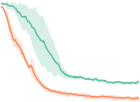
\includegraphics[interpolate=true,width=1.930000in,height=1.410000in]{shape-15-img0.png}}%
\end{pgfscope}%
\begin{pgfscope}%
\pgfsetrectcap%
\pgfsetmiterjoin%
\pgfsetlinewidth{1.254687pt}%
\definecolor{currentstroke}{rgb}{0.150000,0.150000,0.150000}%
\pgfsetstrokecolor{currentstroke}%
\pgfsetdash{}{0pt}%
\pgfpathmoveto{\pgfqpoint{0.695728in}{0.558892in}}%
\pgfpathlineto{\pgfqpoint{0.695728in}{2.098138in}}%
\pgfusepath{stroke}%
\end{pgfscope}%
\begin{pgfscope}%
\pgfsetrectcap%
\pgfsetmiterjoin%
\pgfsetlinewidth{1.254687pt}%
\definecolor{currentstroke}{rgb}{0.150000,0.150000,0.150000}%
\pgfsetstrokecolor{currentstroke}%
\pgfsetdash{}{0pt}%
\pgfpathmoveto{\pgfqpoint{2.790221in}{0.558892in}}%
\pgfpathlineto{\pgfqpoint{2.790221in}{2.098138in}}%
\pgfusepath{stroke}%
\end{pgfscope}%
\begin{pgfscope}%
\pgfsetrectcap%
\pgfsetmiterjoin%
\pgfsetlinewidth{1.254687pt}%
\definecolor{currentstroke}{rgb}{0.150000,0.150000,0.150000}%
\pgfsetstrokecolor{currentstroke}%
\pgfsetdash{}{0pt}%
\pgfpathmoveto{\pgfqpoint{0.695728in}{0.558892in}}%
\pgfpathlineto{\pgfqpoint{2.790221in}{0.558892in}}%
\pgfusepath{stroke}%
\end{pgfscope}%
\begin{pgfscope}%
\pgfsetrectcap%
\pgfsetmiterjoin%
\pgfsetlinewidth{1.254687pt}%
\definecolor{currentstroke}{rgb}{0.150000,0.150000,0.150000}%
\pgfsetstrokecolor{currentstroke}%
\pgfsetdash{}{0pt}%
\pgfpathmoveto{\pgfqpoint{0.695728in}{2.098138in}}%
\pgfpathlineto{\pgfqpoint{2.790221in}{2.098138in}}%
\pgfusepath{stroke}%
\end{pgfscope}%
\begin{pgfscope}%
\pgfsetroundcap%
\pgfsetroundjoin%
\pgfsetlinewidth{1.505625pt}%
\definecolor{currentstroke}{rgb}{0.400000,0.760784,0.647059}%
\pgfsetstrokecolor{currentstroke}%
\pgfsetdash{}{0pt}%
\pgfpathmoveto{\pgfqpoint{2.136379in}{1.952609in}}%
\pgfpathlineto{\pgfqpoint{2.247491in}{1.952609in}}%
\pgfpathlineto{\pgfqpoint{2.358602in}{1.952609in}}%
\pgfusepath{stroke}%
\end{pgfscope}%
\begin{pgfscope}%
\definecolor{textcolor}{rgb}{0.150000,0.150000,0.150000}%
\pgfsetstrokecolor{textcolor}%
\pgfsetfillcolor{textcolor}%
\pgftext[x=2.447491in,y=1.913720in,left,base]{\color{textcolor}\rmfamily\fontsize{8.000000}{9.600000}\selectfont lstm}%
\end{pgfscope}%
\begin{pgfscope}%
\pgfsetroundcap%
\pgfsetroundjoin%
\pgfsetlinewidth{1.505625pt}%
\definecolor{currentstroke}{rgb}{0.988235,0.552941,0.384314}%
\pgfsetstrokecolor{currentstroke}%
\pgfsetdash{}{0pt}%
\pgfpathmoveto{\pgfqpoint{2.136379in}{1.789523in}}%
\pgfpathlineto{\pgfqpoint{2.247491in}{1.789523in}}%
\pgfpathlineto{\pgfqpoint{2.358602in}{1.789523in}}%
\pgfusepath{stroke}%
\end{pgfscope}%
\begin{pgfscope}%
\definecolor{textcolor}{rgb}{0.150000,0.150000,0.150000}%
\pgfsetstrokecolor{textcolor}%
\pgfsetfillcolor{textcolor}%
\pgftext[x=2.447491in,y=1.750634in,left,base]{\color{textcolor}\rmfamily\fontsize{8.000000}{9.600000}\selectfont map}%
\end{pgfscope}%
\begin{pgfscope}%
\pgfsetbuttcap%
\pgfsetmiterjoin%
\definecolor{currentfill}{rgb}{1.000000,1.000000,1.000000}%
\pgfsetfillcolor{currentfill}%
\pgfsetlinewidth{0.000000pt}%
\definecolor{currentstroke}{rgb}{0.000000,0.000000,0.000000}%
\pgfsetstrokecolor{currentstroke}%
\pgfsetstrokeopacity{0.000000}%
\pgfsetdash{}{0pt}%
\pgfpathmoveto{\pgfqpoint{3.401003in}{0.558892in}}%
\pgfpathlineto{\pgfqpoint{5.495496in}{0.558892in}}%
\pgfpathlineto{\pgfqpoint{5.495496in}{2.098138in}}%
\pgfpathlineto{\pgfqpoint{3.401003in}{2.098138in}}%
\pgfpathlineto{\pgfqpoint{3.401003in}{0.558892in}}%
\pgfpathclose%
\pgfusepath{fill}%
\end{pgfscope}%
\begin{pgfscope}%
\pgfsetbuttcap%
\pgfsetroundjoin%
\definecolor{currentfill}{rgb}{0.150000,0.150000,0.150000}%
\pgfsetfillcolor{currentfill}%
\pgfsetlinewidth{1.254687pt}%
\definecolor{currentstroke}{rgb}{0.150000,0.150000,0.150000}%
\pgfsetstrokecolor{currentstroke}%
\pgfsetdash{}{0pt}%
\pgfsys@defobject{currentmarker}{\pgfqpoint{0.000000in}{-0.083333in}}{\pgfqpoint{0.000000in}{0.000000in}}{%
\pgfpathmoveto{\pgfqpoint{0.000000in}{0.000000in}}%
\pgfpathlineto{\pgfqpoint{0.000000in}{-0.083333in}}%
\pgfusepath{stroke,fill}%
}%
\begin{pgfscope}%
\pgfsys@transformshift{3.470871in}{0.558892in}%
\pgfsys@useobject{currentmarker}{}%
\end{pgfscope}%
\end{pgfscope}%
\begin{pgfscope}%
\definecolor{textcolor}{rgb}{0.150000,0.150000,0.150000}%
\pgfsetstrokecolor{textcolor}%
\pgfsetfillcolor{textcolor}%
\pgftext[x=3.470871in,y=0.426948in,,top]{\color{textcolor}\rmfamily\fontsize{8.000000}{9.600000}\selectfont \(\displaystyle {0.0}\)}%
\end{pgfscope}%
\begin{pgfscope}%
\pgfsetbuttcap%
\pgfsetroundjoin%
\definecolor{currentfill}{rgb}{0.150000,0.150000,0.150000}%
\pgfsetfillcolor{currentfill}%
\pgfsetlinewidth{1.254687pt}%
\definecolor{currentstroke}{rgb}{0.150000,0.150000,0.150000}%
\pgfsetstrokecolor{currentstroke}%
\pgfsetdash{}{0pt}%
\pgfsys@defobject{currentmarker}{\pgfqpoint{0.000000in}{-0.083333in}}{\pgfqpoint{0.000000in}{0.000000in}}{%
\pgfpathmoveto{\pgfqpoint{0.000000in}{0.000000in}}%
\pgfpathlineto{\pgfqpoint{0.000000in}{-0.083333in}}%
\pgfusepath{stroke,fill}%
}%
\begin{pgfscope}%
\pgfsys@transformshift{3.857008in}{0.558892in}%
\pgfsys@useobject{currentmarker}{}%
\end{pgfscope}%
\end{pgfscope}%
\begin{pgfscope}%
\definecolor{textcolor}{rgb}{0.150000,0.150000,0.150000}%
\pgfsetstrokecolor{textcolor}%
\pgfsetfillcolor{textcolor}%
\pgftext[x=3.857008in,y=0.426948in,,top]{\color{textcolor}\rmfamily\fontsize{8.000000}{9.600000}\selectfont \(\displaystyle {0.5}\)}%
\end{pgfscope}%
\begin{pgfscope}%
\pgfsetbuttcap%
\pgfsetroundjoin%
\definecolor{currentfill}{rgb}{0.150000,0.150000,0.150000}%
\pgfsetfillcolor{currentfill}%
\pgfsetlinewidth{1.254687pt}%
\definecolor{currentstroke}{rgb}{0.150000,0.150000,0.150000}%
\pgfsetstrokecolor{currentstroke}%
\pgfsetdash{}{0pt}%
\pgfsys@defobject{currentmarker}{\pgfqpoint{0.000000in}{-0.083333in}}{\pgfqpoint{0.000000in}{0.000000in}}{%
\pgfpathmoveto{\pgfqpoint{0.000000in}{0.000000in}}%
\pgfpathlineto{\pgfqpoint{0.000000in}{-0.083333in}}%
\pgfusepath{stroke,fill}%
}%
\begin{pgfscope}%
\pgfsys@transformshift{4.243146in}{0.558892in}%
\pgfsys@useobject{currentmarker}{}%
\end{pgfscope}%
\end{pgfscope}%
\begin{pgfscope}%
\definecolor{textcolor}{rgb}{0.150000,0.150000,0.150000}%
\pgfsetstrokecolor{textcolor}%
\pgfsetfillcolor{textcolor}%
\pgftext[x=4.243146in,y=0.426948in,,top]{\color{textcolor}\rmfamily\fontsize{8.000000}{9.600000}\selectfont \(\displaystyle {1.0}\)}%
\end{pgfscope}%
\begin{pgfscope}%
\pgfsetbuttcap%
\pgfsetroundjoin%
\definecolor{currentfill}{rgb}{0.150000,0.150000,0.150000}%
\pgfsetfillcolor{currentfill}%
\pgfsetlinewidth{1.254687pt}%
\definecolor{currentstroke}{rgb}{0.150000,0.150000,0.150000}%
\pgfsetstrokecolor{currentstroke}%
\pgfsetdash{}{0pt}%
\pgfsys@defobject{currentmarker}{\pgfqpoint{0.000000in}{-0.083333in}}{\pgfqpoint{0.000000in}{0.000000in}}{%
\pgfpathmoveto{\pgfqpoint{0.000000in}{0.000000in}}%
\pgfpathlineto{\pgfqpoint{0.000000in}{-0.083333in}}%
\pgfusepath{stroke,fill}%
}%
\begin{pgfscope}%
\pgfsys@transformshift{4.629283in}{0.558892in}%
\pgfsys@useobject{currentmarker}{}%
\end{pgfscope}%
\end{pgfscope}%
\begin{pgfscope}%
\definecolor{textcolor}{rgb}{0.150000,0.150000,0.150000}%
\pgfsetstrokecolor{textcolor}%
\pgfsetfillcolor{textcolor}%
\pgftext[x=4.629283in,y=0.426948in,,top]{\color{textcolor}\rmfamily\fontsize{8.000000}{9.600000}\selectfont \(\displaystyle {1.5}\)}%
\end{pgfscope}%
\begin{pgfscope}%
\pgfsetbuttcap%
\pgfsetroundjoin%
\definecolor{currentfill}{rgb}{0.150000,0.150000,0.150000}%
\pgfsetfillcolor{currentfill}%
\pgfsetlinewidth{1.254687pt}%
\definecolor{currentstroke}{rgb}{0.150000,0.150000,0.150000}%
\pgfsetstrokecolor{currentstroke}%
\pgfsetdash{}{0pt}%
\pgfsys@defobject{currentmarker}{\pgfqpoint{0.000000in}{-0.083333in}}{\pgfqpoint{0.000000in}{0.000000in}}{%
\pgfpathmoveto{\pgfqpoint{0.000000in}{0.000000in}}%
\pgfpathlineto{\pgfqpoint{0.000000in}{-0.083333in}}%
\pgfusepath{stroke,fill}%
}%
\begin{pgfscope}%
\pgfsys@transformshift{5.015421in}{0.558892in}%
\pgfsys@useobject{currentmarker}{}%
\end{pgfscope}%
\end{pgfscope}%
\begin{pgfscope}%
\definecolor{textcolor}{rgb}{0.150000,0.150000,0.150000}%
\pgfsetstrokecolor{textcolor}%
\pgfsetfillcolor{textcolor}%
\pgftext[x=5.015421in,y=0.426948in,,top]{\color{textcolor}\rmfamily\fontsize{8.000000}{9.600000}\selectfont \(\displaystyle {2.0}\)}%
\end{pgfscope}%
\begin{pgfscope}%
\pgfsetbuttcap%
\pgfsetroundjoin%
\definecolor{currentfill}{rgb}{0.150000,0.150000,0.150000}%
\pgfsetfillcolor{currentfill}%
\pgfsetlinewidth{1.254687pt}%
\definecolor{currentstroke}{rgb}{0.150000,0.150000,0.150000}%
\pgfsetstrokecolor{currentstroke}%
\pgfsetdash{}{0pt}%
\pgfsys@defobject{currentmarker}{\pgfqpoint{0.000000in}{-0.083333in}}{\pgfqpoint{0.000000in}{0.000000in}}{%
\pgfpathmoveto{\pgfqpoint{0.000000in}{0.000000in}}%
\pgfpathlineto{\pgfqpoint{0.000000in}{-0.083333in}}%
\pgfusepath{stroke,fill}%
}%
\begin{pgfscope}%
\pgfsys@transformshift{5.401559in}{0.558892in}%
\pgfsys@useobject{currentmarker}{}%
\end{pgfscope}%
\end{pgfscope}%
\begin{pgfscope}%
\definecolor{textcolor}{rgb}{0.150000,0.150000,0.150000}%
\pgfsetstrokecolor{textcolor}%
\pgfsetfillcolor{textcolor}%
\pgftext[x=5.401559in,y=0.426948in,,top]{\color{textcolor}\rmfamily\fontsize{8.000000}{9.600000}\selectfont \(\displaystyle {2.5}\)}%
\end{pgfscope}%
\begin{pgfscope}%
\definecolor{textcolor}{rgb}{0.150000,0.150000,0.150000}%
\pgfsetstrokecolor{textcolor}%
\pgfsetfillcolor{textcolor}%
\pgftext[x=4.448250in,y=0.263862in,,top]{\color{textcolor}\rmfamily\fontsize{10.000000}{12.000000}\selectfont step}%
\end{pgfscope}%
\begin{pgfscope}%
\definecolor{textcolor}{rgb}{0.150000,0.150000,0.150000}%
\pgfsetstrokecolor{textcolor}%
\pgfsetfillcolor{textcolor}%
\pgftext[x=5.495496in,y=0.277751in,right,top]{\color{textcolor}\rmfamily\fontsize{8.000000}{9.600000}\selectfont \(\displaystyle \times{10^{7}}{}\)}%
\end{pgfscope}%
\begin{pgfscope}%
\pgfsetbuttcap%
\pgfsetroundjoin%
\definecolor{currentfill}{rgb}{0.150000,0.150000,0.150000}%
\pgfsetfillcolor{currentfill}%
\pgfsetlinewidth{1.254687pt}%
\definecolor{currentstroke}{rgb}{0.150000,0.150000,0.150000}%
\pgfsetstrokecolor{currentstroke}%
\pgfsetdash{}{0pt}%
\pgfsys@defobject{currentmarker}{\pgfqpoint{-0.083333in}{0.000000in}}{\pgfqpoint{-0.000000in}{0.000000in}}{%
\pgfpathmoveto{\pgfqpoint{-0.000000in}{0.000000in}}%
\pgfpathlineto{\pgfqpoint{-0.083333in}{0.000000in}}%
\pgfusepath{stroke,fill}%
}%
\begin{pgfscope}%
\pgfsys@transformshift{3.401003in}{0.820395in}%
\pgfsys@useobject{currentmarker}{}%
\end{pgfscope}%
\end{pgfscope}%
\begin{pgfscope}%
\definecolor{textcolor}{rgb}{0.150000,0.150000,0.150000}%
\pgfsetstrokecolor{textcolor}%
\pgfsetfillcolor{textcolor}%
\pgftext[x=3.118208in, y=0.778186in, left, base]{\color{textcolor}\rmfamily\fontsize{8.000000}{9.600000}\selectfont \(\displaystyle {0.2}\)}%
\end{pgfscope}%
\begin{pgfscope}%
\pgfsetbuttcap%
\pgfsetroundjoin%
\definecolor{currentfill}{rgb}{0.150000,0.150000,0.150000}%
\pgfsetfillcolor{currentfill}%
\pgfsetlinewidth{1.254687pt}%
\definecolor{currentstroke}{rgb}{0.150000,0.150000,0.150000}%
\pgfsetstrokecolor{currentstroke}%
\pgfsetdash{}{0pt}%
\pgfsys@defobject{currentmarker}{\pgfqpoint{-0.083333in}{0.000000in}}{\pgfqpoint{-0.000000in}{0.000000in}}{%
\pgfpathmoveto{\pgfqpoint{-0.000000in}{0.000000in}}%
\pgfpathlineto{\pgfqpoint{-0.083333in}{0.000000in}}%
\pgfusepath{stroke,fill}%
}%
\begin{pgfscope}%
\pgfsys@transformshift{3.401003in}{1.122941in}%
\pgfsys@useobject{currentmarker}{}%
\end{pgfscope}%
\end{pgfscope}%
\begin{pgfscope}%
\definecolor{textcolor}{rgb}{0.150000,0.150000,0.150000}%
\pgfsetstrokecolor{textcolor}%
\pgfsetfillcolor{textcolor}%
\pgftext[x=3.118208in, y=1.080732in, left, base]{\color{textcolor}\rmfamily\fontsize{8.000000}{9.600000}\selectfont \(\displaystyle {0.4}\)}%
\end{pgfscope}%
\begin{pgfscope}%
\pgfsetbuttcap%
\pgfsetroundjoin%
\definecolor{currentfill}{rgb}{0.150000,0.150000,0.150000}%
\pgfsetfillcolor{currentfill}%
\pgfsetlinewidth{1.254687pt}%
\definecolor{currentstroke}{rgb}{0.150000,0.150000,0.150000}%
\pgfsetstrokecolor{currentstroke}%
\pgfsetdash{}{0pt}%
\pgfsys@defobject{currentmarker}{\pgfqpoint{-0.083333in}{0.000000in}}{\pgfqpoint{-0.000000in}{0.000000in}}{%
\pgfpathmoveto{\pgfqpoint{-0.000000in}{0.000000in}}%
\pgfpathlineto{\pgfqpoint{-0.083333in}{0.000000in}}%
\pgfusepath{stroke,fill}%
}%
\begin{pgfscope}%
\pgfsys@transformshift{3.401003in}{1.425487in}%
\pgfsys@useobject{currentmarker}{}%
\end{pgfscope}%
\end{pgfscope}%
\begin{pgfscope}%
\definecolor{textcolor}{rgb}{0.150000,0.150000,0.150000}%
\pgfsetstrokecolor{textcolor}%
\pgfsetfillcolor{textcolor}%
\pgftext[x=3.118208in, y=1.383278in, left, base]{\color{textcolor}\rmfamily\fontsize{8.000000}{9.600000}\selectfont \(\displaystyle {0.6}\)}%
\end{pgfscope}%
\begin{pgfscope}%
\pgfsetbuttcap%
\pgfsetroundjoin%
\definecolor{currentfill}{rgb}{0.150000,0.150000,0.150000}%
\pgfsetfillcolor{currentfill}%
\pgfsetlinewidth{1.254687pt}%
\definecolor{currentstroke}{rgb}{0.150000,0.150000,0.150000}%
\pgfsetstrokecolor{currentstroke}%
\pgfsetdash{}{0pt}%
\pgfsys@defobject{currentmarker}{\pgfqpoint{-0.083333in}{0.000000in}}{\pgfqpoint{-0.000000in}{0.000000in}}{%
\pgfpathmoveto{\pgfqpoint{-0.000000in}{0.000000in}}%
\pgfpathlineto{\pgfqpoint{-0.083333in}{0.000000in}}%
\pgfusepath{stroke,fill}%
}%
\begin{pgfscope}%
\pgfsys@transformshift{3.401003in}{1.728033in}%
\pgfsys@useobject{currentmarker}{}%
\end{pgfscope}%
\end{pgfscope}%
\begin{pgfscope}%
\definecolor{textcolor}{rgb}{0.150000,0.150000,0.150000}%
\pgfsetstrokecolor{textcolor}%
\pgfsetfillcolor{textcolor}%
\pgftext[x=3.118208in, y=1.685824in, left, base]{\color{textcolor}\rmfamily\fontsize{8.000000}{9.600000}\selectfont \(\displaystyle {0.8}\)}%
\end{pgfscope}%
\begin{pgfscope}%
\pgfsetbuttcap%
\pgfsetroundjoin%
\definecolor{currentfill}{rgb}{0.150000,0.150000,0.150000}%
\pgfsetfillcolor{currentfill}%
\pgfsetlinewidth{1.254687pt}%
\definecolor{currentstroke}{rgb}{0.150000,0.150000,0.150000}%
\pgfsetstrokecolor{currentstroke}%
\pgfsetdash{}{0pt}%
\pgfsys@defobject{currentmarker}{\pgfqpoint{-0.083333in}{0.000000in}}{\pgfqpoint{-0.000000in}{0.000000in}}{%
\pgfpathmoveto{\pgfqpoint{-0.000000in}{0.000000in}}%
\pgfpathlineto{\pgfqpoint{-0.083333in}{0.000000in}}%
\pgfusepath{stroke,fill}%
}%
\begin{pgfscope}%
\pgfsys@transformshift{3.401003in}{2.030580in}%
\pgfsys@useobject{currentmarker}{}%
\end{pgfscope}%
\end{pgfscope}%
\begin{pgfscope}%
\definecolor{textcolor}{rgb}{0.150000,0.150000,0.150000}%
\pgfsetstrokecolor{textcolor}%
\pgfsetfillcolor{textcolor}%
\pgftext[x=3.118208in, y=1.988370in, left, base]{\color{textcolor}\rmfamily\fontsize{8.000000}{9.600000}\selectfont \(\displaystyle {1.0}\)}%
\end{pgfscope}%
\begin{pgfscope}%
\definecolor{textcolor}{rgb}{0.150000,0.150000,0.150000}%
\pgfsetstrokecolor{textcolor}%
\pgfsetfillcolor{textcolor}%
\pgftext[x=3.062652in,y=1.328515in,,bottom,rotate=90.000000]{\color{textcolor}\rmfamily\fontsize{10.000000}{12.000000}\selectfont success}%
\end{pgfscope}%
\begin{pgfscope}%
\pgfsys@transformshift{3.480000in}{0.628198in}%
\pgftext[left,bottom]{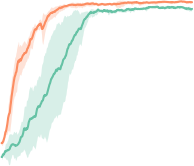
\includegraphics[interpolate=true,width=1.940000in,height=1.410000in]{shape-15-img1.png}}%
\end{pgfscope}%
\begin{pgfscope}%
\pgfsetrectcap%
\pgfsetmiterjoin%
\pgfsetlinewidth{1.254687pt}%
\definecolor{currentstroke}{rgb}{0.150000,0.150000,0.150000}%
\pgfsetstrokecolor{currentstroke}%
\pgfsetdash{}{0pt}%
\pgfpathmoveto{\pgfqpoint{3.401003in}{0.558892in}}%
\pgfpathlineto{\pgfqpoint{3.401003in}{2.098138in}}%
\pgfusepath{stroke}%
\end{pgfscope}%
\begin{pgfscope}%
\pgfsetrectcap%
\pgfsetmiterjoin%
\pgfsetlinewidth{1.254687pt}%
\definecolor{currentstroke}{rgb}{0.150000,0.150000,0.150000}%
\pgfsetstrokecolor{currentstroke}%
\pgfsetdash{}{0pt}%
\pgfpathmoveto{\pgfqpoint{5.495496in}{0.558892in}}%
\pgfpathlineto{\pgfqpoint{5.495496in}{2.098138in}}%
\pgfusepath{stroke}%
\end{pgfscope}%
\begin{pgfscope}%
\pgfsetrectcap%
\pgfsetmiterjoin%
\pgfsetlinewidth{1.254687pt}%
\definecolor{currentstroke}{rgb}{0.150000,0.150000,0.150000}%
\pgfsetstrokecolor{currentstroke}%
\pgfsetdash{}{0pt}%
\pgfpathmoveto{\pgfqpoint{3.401003in}{0.558892in}}%
\pgfpathlineto{\pgfqpoint{5.495496in}{0.558892in}}%
\pgfusepath{stroke}%
\end{pgfscope}%
\begin{pgfscope}%
\pgfsetrectcap%
\pgfsetmiterjoin%
\pgfsetlinewidth{1.254687pt}%
\definecolor{currentstroke}{rgb}{0.150000,0.150000,0.150000}%
\pgfsetstrokecolor{currentstroke}%
\pgfsetdash{}{0pt}%
\pgfpathmoveto{\pgfqpoint{3.401003in}{2.098138in}}%
\pgfpathlineto{\pgfqpoint{5.495496in}{2.098138in}}%
\pgfusepath{stroke}%
\end{pgfscope}%
\begin{pgfscope}%
\pgfsetroundcap%
\pgfsetroundjoin%
\pgfsetlinewidth{1.505625pt}%
\definecolor{currentstroke}{rgb}{0.400000,0.760784,0.647059}%
\pgfsetstrokecolor{currentstroke}%
\pgfsetdash{}{0pt}%
\pgfpathmoveto{\pgfqpoint{4.841655in}{0.883979in}}%
\pgfpathlineto{\pgfqpoint{4.952766in}{0.883979in}}%
\pgfpathlineto{\pgfqpoint{5.063877in}{0.883979in}}%
\pgfusepath{stroke}%
\end{pgfscope}%
\begin{pgfscope}%
\definecolor{textcolor}{rgb}{0.150000,0.150000,0.150000}%
\pgfsetstrokecolor{textcolor}%
\pgfsetfillcolor{textcolor}%
\pgftext[x=5.152766in,y=0.845090in,left,base]{\color{textcolor}\rmfamily\fontsize{8.000000}{9.600000}\selectfont lstm}%
\end{pgfscope}%
\begin{pgfscope}%
\pgfsetroundcap%
\pgfsetroundjoin%
\pgfsetlinewidth{1.505625pt}%
\definecolor{currentstroke}{rgb}{0.988235,0.552941,0.384314}%
\pgfsetstrokecolor{currentstroke}%
\pgfsetdash{}{0pt}%
\pgfpathmoveto{\pgfqpoint{4.841655in}{0.720893in}}%
\pgfpathlineto{\pgfqpoint{4.952766in}{0.720893in}}%
\pgfpathlineto{\pgfqpoint{5.063877in}{0.720893in}}%
\pgfusepath{stroke}%
\end{pgfscope}%
\begin{pgfscope}%
\definecolor{textcolor}{rgb}{0.150000,0.150000,0.150000}%
\pgfsetstrokecolor{textcolor}%
\pgfsetfillcolor{textcolor}%
\pgftext[x=5.152766in,y=0.682004in,left,base]{\color{textcolor}\rmfamily\fontsize{8.000000}{9.600000}\selectfont map}%
\end{pgfscope}%
\end{pgfpicture}%
\makeatother%
\endgroup%

    \(20 \times 20\)
    %% Creator: Matplotlib, PGF backend
%%
%% To include the figure in your LaTeX document, write
%%   \input{<filename>.pgf}
%%
%% Make sure the required packages are loaded in your preamble
%%   \usepackage{pgf}
%%
%% Also ensure that all the required font packages are loaded; for instance,
%% the lmodern package is sometimes necessary when using math font.
%%   \usepackage{lmodern}
%%
%% Figures using additional raster images can only be included by \input if
%% they are in the same directory as the main LaTeX file. For loading figures
%% from other directories you can use the `import` package
%%   \usepackage{import}
%%
%% and then include the figures with
%%   \import{<path to file>}{<filename>.pgf}
%%
%% Matplotlib used the following preamble
%%   \usepackage{fontspec}
%%   \setmainfont{DejaVuSerif.ttf}[Path=\detokenize{/home/oslund/.local/lib/python3.8/site-packages/matplotlib/mpl-data/fonts/ttf/}]
%%   \setsansfont{DejaVuSans.ttf}[Path=\detokenize{/home/oslund/.local/lib/python3.8/site-packages/matplotlib/mpl-data/fonts/ttf/}]
%%   \setmonofont{DejaVuSansMono.ttf}[Path=\detokenize{/home/oslund/.local/lib/python3.8/site-packages/matplotlib/mpl-data/fonts/ttf/}]
%%
\begingroup%
\makeatletter%
\begin{pgfpicture}%
\pgfpathrectangle{\pgfpointorigin}{\pgfqpoint{5.645496in}{3.489108in}}%
\pgfusepath{use as bounding box, clip}%
\begin{pgfscope}%
\pgfsetbuttcap%
\pgfsetmiterjoin%
\definecolor{currentfill}{rgb}{1.000000,1.000000,1.000000}%
\pgfsetfillcolor{currentfill}%
\pgfsetlinewidth{0.000000pt}%
\definecolor{currentstroke}{rgb}{1.000000,1.000000,1.000000}%
\pgfsetstrokecolor{currentstroke}%
\pgfsetdash{}{0pt}%
\pgfpathmoveto{\pgfqpoint{0.000000in}{0.000000in}}%
\pgfpathlineto{\pgfqpoint{5.645496in}{0.000000in}}%
\pgfpathlineto{\pgfqpoint{5.645496in}{3.489108in}}%
\pgfpathlineto{\pgfqpoint{0.000000in}{3.489108in}}%
\pgfpathlineto{\pgfqpoint{0.000000in}{0.000000in}}%
\pgfpathclose%
\pgfusepath{fill}%
\end{pgfscope}%
\begin{pgfscope}%
\pgfsetbuttcap%
\pgfsetmiterjoin%
\definecolor{currentfill}{rgb}{1.000000,1.000000,1.000000}%
\pgfsetfillcolor{currentfill}%
\pgfsetlinewidth{0.000000pt}%
\definecolor{currentstroke}{rgb}{0.000000,0.000000,0.000000}%
\pgfsetstrokecolor{currentstroke}%
\pgfsetstrokeopacity{0.000000}%
\pgfsetdash{}{0pt}%
\pgfpathmoveto{\pgfqpoint{0.661006in}{0.524170in}}%
\pgfpathlineto{\pgfqpoint{2.790221in}{0.524170in}}%
\pgfpathlineto{\pgfqpoint{2.790221in}{3.041514in}}%
\pgfpathlineto{\pgfqpoint{0.661006in}{3.041514in}}%
\pgfpathlineto{\pgfqpoint{0.661006in}{0.524170in}}%
\pgfpathclose%
\pgfusepath{fill}%
\end{pgfscope}%
\begin{pgfscope}%
\pgfsys@transformshift{0.760000in}{0.639108in}%
\pgftext[left,bottom]{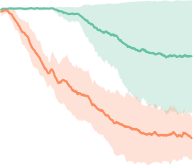
\includegraphics[interpolate=true,width=1.940000in,height=2.300000in]{shape-20-img0.png}}%
\end{pgfscope}%
\begin{pgfscope}%
\pgfsetbuttcap%
\pgfsetroundjoin%
\definecolor{currentfill}{rgb}{0.000000,0.000000,0.000000}%
\pgfsetfillcolor{currentfill}%
\pgfsetlinewidth{0.803000pt}%
\definecolor{currentstroke}{rgb}{0.000000,0.000000,0.000000}%
\pgfsetstrokecolor{currentstroke}%
\pgfsetdash{}{0pt}%
\pgfsys@defobject{currentmarker}{\pgfqpoint{0.000000in}{-0.048611in}}{\pgfqpoint{0.000000in}{0.000000in}}{%
\pgfpathmoveto{\pgfqpoint{0.000000in}{0.000000in}}%
\pgfpathlineto{\pgfqpoint{0.000000in}{-0.048611in}}%
\pgfusepath{stroke,fill}%
}%
\begin{pgfscope}%
\pgfsys@transformshift{0.732031in}{0.524170in}%
\pgfsys@useobject{currentmarker}{}%
\end{pgfscope}%
\end{pgfscope}%
\begin{pgfscope}%
\definecolor{textcolor}{rgb}{0.000000,0.000000,0.000000}%
\pgfsetstrokecolor{textcolor}%
\pgfsetfillcolor{textcolor}%
\pgftext[x=0.732031in,y=0.426948in,,top]{\color{textcolor}\rmfamily\fontsize{8.000000}{9.600000}\selectfont \(\displaystyle {0.0}\)}%
\end{pgfscope}%
\begin{pgfscope}%
\pgfsetbuttcap%
\pgfsetroundjoin%
\definecolor{currentfill}{rgb}{0.000000,0.000000,0.000000}%
\pgfsetfillcolor{currentfill}%
\pgfsetlinewidth{0.803000pt}%
\definecolor{currentstroke}{rgb}{0.000000,0.000000,0.000000}%
\pgfsetstrokecolor{currentstroke}%
\pgfsetdash{}{0pt}%
\pgfsys@defobject{currentmarker}{\pgfqpoint{0.000000in}{-0.048611in}}{\pgfqpoint{0.000000in}{0.000000in}}{%
\pgfpathmoveto{\pgfqpoint{0.000000in}{0.000000in}}%
\pgfpathlineto{\pgfqpoint{0.000000in}{-0.048611in}}%
\pgfusepath{stroke,fill}%
}%
\begin{pgfscope}%
\pgfsys@transformshift{1.124570in}{0.524170in}%
\pgfsys@useobject{currentmarker}{}%
\end{pgfscope}%
\end{pgfscope}%
\begin{pgfscope}%
\definecolor{textcolor}{rgb}{0.000000,0.000000,0.000000}%
\pgfsetstrokecolor{textcolor}%
\pgfsetfillcolor{textcolor}%
\pgftext[x=1.124570in,y=0.426948in,,top]{\color{textcolor}\rmfamily\fontsize{8.000000}{9.600000}\selectfont \(\displaystyle {0.5}\)}%
\end{pgfscope}%
\begin{pgfscope}%
\pgfsetbuttcap%
\pgfsetroundjoin%
\definecolor{currentfill}{rgb}{0.000000,0.000000,0.000000}%
\pgfsetfillcolor{currentfill}%
\pgfsetlinewidth{0.803000pt}%
\definecolor{currentstroke}{rgb}{0.000000,0.000000,0.000000}%
\pgfsetstrokecolor{currentstroke}%
\pgfsetdash{}{0pt}%
\pgfsys@defobject{currentmarker}{\pgfqpoint{0.000000in}{-0.048611in}}{\pgfqpoint{0.000000in}{0.000000in}}{%
\pgfpathmoveto{\pgfqpoint{0.000000in}{0.000000in}}%
\pgfpathlineto{\pgfqpoint{0.000000in}{-0.048611in}}%
\pgfusepath{stroke,fill}%
}%
\begin{pgfscope}%
\pgfsys@transformshift{1.517109in}{0.524170in}%
\pgfsys@useobject{currentmarker}{}%
\end{pgfscope}%
\end{pgfscope}%
\begin{pgfscope}%
\definecolor{textcolor}{rgb}{0.000000,0.000000,0.000000}%
\pgfsetstrokecolor{textcolor}%
\pgfsetfillcolor{textcolor}%
\pgftext[x=1.517109in,y=0.426948in,,top]{\color{textcolor}\rmfamily\fontsize{8.000000}{9.600000}\selectfont \(\displaystyle {1.0}\)}%
\end{pgfscope}%
\begin{pgfscope}%
\pgfsetbuttcap%
\pgfsetroundjoin%
\definecolor{currentfill}{rgb}{0.000000,0.000000,0.000000}%
\pgfsetfillcolor{currentfill}%
\pgfsetlinewidth{0.803000pt}%
\definecolor{currentstroke}{rgb}{0.000000,0.000000,0.000000}%
\pgfsetstrokecolor{currentstroke}%
\pgfsetdash{}{0pt}%
\pgfsys@defobject{currentmarker}{\pgfqpoint{0.000000in}{-0.048611in}}{\pgfqpoint{0.000000in}{0.000000in}}{%
\pgfpathmoveto{\pgfqpoint{0.000000in}{0.000000in}}%
\pgfpathlineto{\pgfqpoint{0.000000in}{-0.048611in}}%
\pgfusepath{stroke,fill}%
}%
\begin{pgfscope}%
\pgfsys@transformshift{1.909648in}{0.524170in}%
\pgfsys@useobject{currentmarker}{}%
\end{pgfscope}%
\end{pgfscope}%
\begin{pgfscope}%
\definecolor{textcolor}{rgb}{0.000000,0.000000,0.000000}%
\pgfsetstrokecolor{textcolor}%
\pgfsetfillcolor{textcolor}%
\pgftext[x=1.909648in,y=0.426948in,,top]{\color{textcolor}\rmfamily\fontsize{8.000000}{9.600000}\selectfont \(\displaystyle {1.5}\)}%
\end{pgfscope}%
\begin{pgfscope}%
\pgfsetbuttcap%
\pgfsetroundjoin%
\definecolor{currentfill}{rgb}{0.000000,0.000000,0.000000}%
\pgfsetfillcolor{currentfill}%
\pgfsetlinewidth{0.803000pt}%
\definecolor{currentstroke}{rgb}{0.000000,0.000000,0.000000}%
\pgfsetstrokecolor{currentstroke}%
\pgfsetdash{}{0pt}%
\pgfsys@defobject{currentmarker}{\pgfqpoint{0.000000in}{-0.048611in}}{\pgfqpoint{0.000000in}{0.000000in}}{%
\pgfpathmoveto{\pgfqpoint{0.000000in}{0.000000in}}%
\pgfpathlineto{\pgfqpoint{0.000000in}{-0.048611in}}%
\pgfusepath{stroke,fill}%
}%
\begin{pgfscope}%
\pgfsys@transformshift{2.302187in}{0.524170in}%
\pgfsys@useobject{currentmarker}{}%
\end{pgfscope}%
\end{pgfscope}%
\begin{pgfscope}%
\definecolor{textcolor}{rgb}{0.000000,0.000000,0.000000}%
\pgfsetstrokecolor{textcolor}%
\pgfsetfillcolor{textcolor}%
\pgftext[x=2.302187in,y=0.426948in,,top]{\color{textcolor}\rmfamily\fontsize{8.000000}{9.600000}\selectfont \(\displaystyle {2.0}\)}%
\end{pgfscope}%
\begin{pgfscope}%
\pgfsetbuttcap%
\pgfsetroundjoin%
\definecolor{currentfill}{rgb}{0.000000,0.000000,0.000000}%
\pgfsetfillcolor{currentfill}%
\pgfsetlinewidth{0.803000pt}%
\definecolor{currentstroke}{rgb}{0.000000,0.000000,0.000000}%
\pgfsetstrokecolor{currentstroke}%
\pgfsetdash{}{0pt}%
\pgfsys@defobject{currentmarker}{\pgfqpoint{0.000000in}{-0.048611in}}{\pgfqpoint{0.000000in}{0.000000in}}{%
\pgfpathmoveto{\pgfqpoint{0.000000in}{0.000000in}}%
\pgfpathlineto{\pgfqpoint{0.000000in}{-0.048611in}}%
\pgfusepath{stroke,fill}%
}%
\begin{pgfscope}%
\pgfsys@transformshift{2.694726in}{0.524170in}%
\pgfsys@useobject{currentmarker}{}%
\end{pgfscope}%
\end{pgfscope}%
\begin{pgfscope}%
\definecolor{textcolor}{rgb}{0.000000,0.000000,0.000000}%
\pgfsetstrokecolor{textcolor}%
\pgfsetfillcolor{textcolor}%
\pgftext[x=2.694726in,y=0.426948in,,top]{\color{textcolor}\rmfamily\fontsize{8.000000}{9.600000}\selectfont \(\displaystyle {2.5}\)}%
\end{pgfscope}%
\begin{pgfscope}%
\definecolor{textcolor}{rgb}{0.000000,0.000000,0.000000}%
\pgfsetstrokecolor{textcolor}%
\pgfsetfillcolor{textcolor}%
\pgftext[x=1.725613in,y=0.263862in,,top]{\color{textcolor}\rmfamily\fontsize{10.000000}{12.000000}\selectfont step}%
\end{pgfscope}%
\begin{pgfscope}%
\definecolor{textcolor}{rgb}{0.000000,0.000000,0.000000}%
\pgfsetstrokecolor{textcolor}%
\pgfsetfillcolor{textcolor}%
\pgftext[x=2.790221in,y=0.277751in,right,top]{\color{textcolor}\rmfamily\fontsize{8.000000}{9.600000}\selectfont \(\displaystyle \times{10^{7}}{}\)}%
\end{pgfscope}%
\begin{pgfscope}%
\pgfsetbuttcap%
\pgfsetroundjoin%
\definecolor{currentfill}{rgb}{0.000000,0.000000,0.000000}%
\pgfsetfillcolor{currentfill}%
\pgfsetlinewidth{0.803000pt}%
\definecolor{currentstroke}{rgb}{0.000000,0.000000,0.000000}%
\pgfsetstrokecolor{currentstroke}%
\pgfsetdash{}{0pt}%
\pgfsys@defobject{currentmarker}{\pgfqpoint{-0.048611in}{0.000000in}}{\pgfqpoint{-0.000000in}{0.000000in}}{%
\pgfpathmoveto{\pgfqpoint{-0.000000in}{0.000000in}}%
\pgfpathlineto{\pgfqpoint{-0.048611in}{0.000000in}}%
\pgfusepath{stroke,fill}%
}%
\begin{pgfscope}%
\pgfsys@transformshift{0.661006in}{0.676684in}%
\pgfsys@useobject{currentmarker}{}%
\end{pgfscope}%
\end{pgfscope}%
\begin{pgfscope}%
\definecolor{textcolor}{rgb}{0.000000,0.000000,0.000000}%
\pgfsetstrokecolor{textcolor}%
\pgfsetfillcolor{textcolor}%
\pgftext[x=0.386698in, y=0.634474in, left, base]{\color{textcolor}\rmfamily\fontsize{8.000000}{9.600000}\selectfont \(\displaystyle {300}\)}%
\end{pgfscope}%
\begin{pgfscope}%
\pgfsetbuttcap%
\pgfsetroundjoin%
\definecolor{currentfill}{rgb}{0.000000,0.000000,0.000000}%
\pgfsetfillcolor{currentfill}%
\pgfsetlinewidth{0.803000pt}%
\definecolor{currentstroke}{rgb}{0.000000,0.000000,0.000000}%
\pgfsetstrokecolor{currentstroke}%
\pgfsetdash{}{0pt}%
\pgfsys@defobject{currentmarker}{\pgfqpoint{-0.048611in}{0.000000in}}{\pgfqpoint{-0.000000in}{0.000000in}}{%
\pgfpathmoveto{\pgfqpoint{-0.000000in}{0.000000in}}%
\pgfpathlineto{\pgfqpoint{-0.048611in}{0.000000in}}%
\pgfusepath{stroke,fill}%
}%
\begin{pgfscope}%
\pgfsys@transformshift{0.661006in}{0.983538in}%
\pgfsys@useobject{currentmarker}{}%
\end{pgfscope}%
\end{pgfscope}%
\begin{pgfscope}%
\definecolor{textcolor}{rgb}{0.000000,0.000000,0.000000}%
\pgfsetstrokecolor{textcolor}%
\pgfsetfillcolor{textcolor}%
\pgftext[x=0.386698in, y=0.941329in, left, base]{\color{textcolor}\rmfamily\fontsize{8.000000}{9.600000}\selectfont \(\displaystyle {400}\)}%
\end{pgfscope}%
\begin{pgfscope}%
\pgfsetbuttcap%
\pgfsetroundjoin%
\definecolor{currentfill}{rgb}{0.000000,0.000000,0.000000}%
\pgfsetfillcolor{currentfill}%
\pgfsetlinewidth{0.803000pt}%
\definecolor{currentstroke}{rgb}{0.000000,0.000000,0.000000}%
\pgfsetstrokecolor{currentstroke}%
\pgfsetdash{}{0pt}%
\pgfsys@defobject{currentmarker}{\pgfqpoint{-0.048611in}{0.000000in}}{\pgfqpoint{-0.000000in}{0.000000in}}{%
\pgfpathmoveto{\pgfqpoint{-0.000000in}{0.000000in}}%
\pgfpathlineto{\pgfqpoint{-0.048611in}{0.000000in}}%
\pgfusepath{stroke,fill}%
}%
\begin{pgfscope}%
\pgfsys@transformshift{0.661006in}{1.290393in}%
\pgfsys@useobject{currentmarker}{}%
\end{pgfscope}%
\end{pgfscope}%
\begin{pgfscope}%
\definecolor{textcolor}{rgb}{0.000000,0.000000,0.000000}%
\pgfsetstrokecolor{textcolor}%
\pgfsetfillcolor{textcolor}%
\pgftext[x=0.386698in, y=1.248184in, left, base]{\color{textcolor}\rmfamily\fontsize{8.000000}{9.600000}\selectfont \(\displaystyle {500}\)}%
\end{pgfscope}%
\begin{pgfscope}%
\pgfsetbuttcap%
\pgfsetroundjoin%
\definecolor{currentfill}{rgb}{0.000000,0.000000,0.000000}%
\pgfsetfillcolor{currentfill}%
\pgfsetlinewidth{0.803000pt}%
\definecolor{currentstroke}{rgb}{0.000000,0.000000,0.000000}%
\pgfsetstrokecolor{currentstroke}%
\pgfsetdash{}{0pt}%
\pgfsys@defobject{currentmarker}{\pgfqpoint{-0.048611in}{0.000000in}}{\pgfqpoint{-0.000000in}{0.000000in}}{%
\pgfpathmoveto{\pgfqpoint{-0.000000in}{0.000000in}}%
\pgfpathlineto{\pgfqpoint{-0.048611in}{0.000000in}}%
\pgfusepath{stroke,fill}%
}%
\begin{pgfscope}%
\pgfsys@transformshift{0.661006in}{1.597248in}%
\pgfsys@useobject{currentmarker}{}%
\end{pgfscope}%
\end{pgfscope}%
\begin{pgfscope}%
\definecolor{textcolor}{rgb}{0.000000,0.000000,0.000000}%
\pgfsetstrokecolor{textcolor}%
\pgfsetfillcolor{textcolor}%
\pgftext[x=0.386698in, y=1.555039in, left, base]{\color{textcolor}\rmfamily\fontsize{8.000000}{9.600000}\selectfont \(\displaystyle {600}\)}%
\end{pgfscope}%
\begin{pgfscope}%
\pgfsetbuttcap%
\pgfsetroundjoin%
\definecolor{currentfill}{rgb}{0.000000,0.000000,0.000000}%
\pgfsetfillcolor{currentfill}%
\pgfsetlinewidth{0.803000pt}%
\definecolor{currentstroke}{rgb}{0.000000,0.000000,0.000000}%
\pgfsetstrokecolor{currentstroke}%
\pgfsetdash{}{0pt}%
\pgfsys@defobject{currentmarker}{\pgfqpoint{-0.048611in}{0.000000in}}{\pgfqpoint{-0.000000in}{0.000000in}}{%
\pgfpathmoveto{\pgfqpoint{-0.000000in}{0.000000in}}%
\pgfpathlineto{\pgfqpoint{-0.048611in}{0.000000in}}%
\pgfusepath{stroke,fill}%
}%
\begin{pgfscope}%
\pgfsys@transformshift{0.661006in}{1.904103in}%
\pgfsys@useobject{currentmarker}{}%
\end{pgfscope}%
\end{pgfscope}%
\begin{pgfscope}%
\definecolor{textcolor}{rgb}{0.000000,0.000000,0.000000}%
\pgfsetstrokecolor{textcolor}%
\pgfsetfillcolor{textcolor}%
\pgftext[x=0.386698in, y=1.861893in, left, base]{\color{textcolor}\rmfamily\fontsize{8.000000}{9.600000}\selectfont \(\displaystyle {700}\)}%
\end{pgfscope}%
\begin{pgfscope}%
\pgfsetbuttcap%
\pgfsetroundjoin%
\definecolor{currentfill}{rgb}{0.000000,0.000000,0.000000}%
\pgfsetfillcolor{currentfill}%
\pgfsetlinewidth{0.803000pt}%
\definecolor{currentstroke}{rgb}{0.000000,0.000000,0.000000}%
\pgfsetstrokecolor{currentstroke}%
\pgfsetdash{}{0pt}%
\pgfsys@defobject{currentmarker}{\pgfqpoint{-0.048611in}{0.000000in}}{\pgfqpoint{-0.000000in}{0.000000in}}{%
\pgfpathmoveto{\pgfqpoint{-0.000000in}{0.000000in}}%
\pgfpathlineto{\pgfqpoint{-0.048611in}{0.000000in}}%
\pgfusepath{stroke,fill}%
}%
\begin{pgfscope}%
\pgfsys@transformshift{0.661006in}{2.210957in}%
\pgfsys@useobject{currentmarker}{}%
\end{pgfscope}%
\end{pgfscope}%
\begin{pgfscope}%
\definecolor{textcolor}{rgb}{0.000000,0.000000,0.000000}%
\pgfsetstrokecolor{textcolor}%
\pgfsetfillcolor{textcolor}%
\pgftext[x=0.386698in, y=2.168748in, left, base]{\color{textcolor}\rmfamily\fontsize{8.000000}{9.600000}\selectfont \(\displaystyle {800}\)}%
\end{pgfscope}%
\begin{pgfscope}%
\pgfsetbuttcap%
\pgfsetroundjoin%
\definecolor{currentfill}{rgb}{0.000000,0.000000,0.000000}%
\pgfsetfillcolor{currentfill}%
\pgfsetlinewidth{0.803000pt}%
\definecolor{currentstroke}{rgb}{0.000000,0.000000,0.000000}%
\pgfsetstrokecolor{currentstroke}%
\pgfsetdash{}{0pt}%
\pgfsys@defobject{currentmarker}{\pgfqpoint{-0.048611in}{0.000000in}}{\pgfqpoint{-0.000000in}{0.000000in}}{%
\pgfpathmoveto{\pgfqpoint{-0.000000in}{0.000000in}}%
\pgfpathlineto{\pgfqpoint{-0.048611in}{0.000000in}}%
\pgfusepath{stroke,fill}%
}%
\begin{pgfscope}%
\pgfsys@transformshift{0.661006in}{2.517812in}%
\pgfsys@useobject{currentmarker}{}%
\end{pgfscope}%
\end{pgfscope}%
\begin{pgfscope}%
\definecolor{textcolor}{rgb}{0.000000,0.000000,0.000000}%
\pgfsetstrokecolor{textcolor}%
\pgfsetfillcolor{textcolor}%
\pgftext[x=0.386698in, y=2.475603in, left, base]{\color{textcolor}\rmfamily\fontsize{8.000000}{9.600000}\selectfont \(\displaystyle {900}\)}%
\end{pgfscope}%
\begin{pgfscope}%
\pgfsetbuttcap%
\pgfsetroundjoin%
\definecolor{currentfill}{rgb}{0.000000,0.000000,0.000000}%
\pgfsetfillcolor{currentfill}%
\pgfsetlinewidth{0.803000pt}%
\definecolor{currentstroke}{rgb}{0.000000,0.000000,0.000000}%
\pgfsetstrokecolor{currentstroke}%
\pgfsetdash{}{0pt}%
\pgfsys@defobject{currentmarker}{\pgfqpoint{-0.048611in}{0.000000in}}{\pgfqpoint{-0.000000in}{0.000000in}}{%
\pgfpathmoveto{\pgfqpoint{-0.000000in}{0.000000in}}%
\pgfpathlineto{\pgfqpoint{-0.048611in}{0.000000in}}%
\pgfusepath{stroke,fill}%
}%
\begin{pgfscope}%
\pgfsys@transformshift{0.661006in}{2.824667in}%
\pgfsys@useobject{currentmarker}{}%
\end{pgfscope}%
\end{pgfscope}%
\begin{pgfscope}%
\definecolor{textcolor}{rgb}{0.000000,0.000000,0.000000}%
\pgfsetstrokecolor{textcolor}%
\pgfsetfillcolor{textcolor}%
\pgftext[x=0.327669in, y=2.782457in, left, base]{\color{textcolor}\rmfamily\fontsize{8.000000}{9.600000}\selectfont \(\displaystyle {1000}\)}%
\end{pgfscope}%
\begin{pgfscope}%
\definecolor{textcolor}{rgb}{0.000000,0.000000,0.000000}%
\pgfsetstrokecolor{textcolor}%
\pgfsetfillcolor{textcolor}%
\pgftext[x=0.272113in,y=1.782842in,,bottom,rotate=90.000000]{\color{textcolor}\rmfamily\fontsize{10.000000}{12.000000}\selectfont length}%
\end{pgfscope}%
\begin{pgfscope}%
\pgfsys@transformshift{0.740000in}{0.999108in}%
\pgftext[left,bottom]{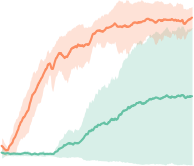
\includegraphics[interpolate=true,width=1.970000in,height=1.840000in]{shape-20-img1.png}}%
\end{pgfscope}%
\begin{pgfscope}%
\pgfsetrectcap%
\pgfsetmiterjoin%
\pgfsetlinewidth{0.803000pt}%
\definecolor{currentstroke}{rgb}{0.000000,0.000000,0.000000}%
\pgfsetstrokecolor{currentstroke}%
\pgfsetdash{}{0pt}%
\pgfpathmoveto{\pgfqpoint{0.661006in}{0.524170in}}%
\pgfpathlineto{\pgfqpoint{0.661006in}{3.041514in}}%
\pgfusepath{stroke}%
\end{pgfscope}%
\begin{pgfscope}%
\pgfsetrectcap%
\pgfsetmiterjoin%
\pgfsetlinewidth{0.803000pt}%
\definecolor{currentstroke}{rgb}{0.000000,0.000000,0.000000}%
\pgfsetstrokecolor{currentstroke}%
\pgfsetdash{}{0pt}%
\pgfpathmoveto{\pgfqpoint{2.790221in}{0.524170in}}%
\pgfpathlineto{\pgfqpoint{2.790221in}{3.041514in}}%
\pgfusepath{stroke}%
\end{pgfscope}%
\begin{pgfscope}%
\pgfsetrectcap%
\pgfsetmiterjoin%
\pgfsetlinewidth{0.803000pt}%
\definecolor{currentstroke}{rgb}{0.000000,0.000000,0.000000}%
\pgfsetstrokecolor{currentstroke}%
\pgfsetdash{}{0pt}%
\pgfpathmoveto{\pgfqpoint{0.661006in}{0.524170in}}%
\pgfpathlineto{\pgfqpoint{2.790221in}{0.524170in}}%
\pgfusepath{stroke}%
\end{pgfscope}%
\begin{pgfscope}%
\pgfsetrectcap%
\pgfsetmiterjoin%
\pgfsetlinewidth{0.803000pt}%
\definecolor{currentstroke}{rgb}{0.000000,0.000000,0.000000}%
\pgfsetstrokecolor{currentstroke}%
\pgfsetdash{}{0pt}%
\pgfpathmoveto{\pgfqpoint{0.661006in}{3.041514in}}%
\pgfpathlineto{\pgfqpoint{2.790221in}{3.041514in}}%
\pgfusepath{stroke}%
\end{pgfscope}%
\begin{pgfscope}%
\pgfsetrectcap%
\pgfsetroundjoin%
\pgfsetlinewidth{1.505625pt}%
\definecolor{currentstroke}{rgb}{0.000000,0.419608,0.643137}%
\pgfsetstrokecolor{currentstroke}%
\pgfsetdash{}{0pt}%
\pgfpathmoveto{\pgfqpoint{2.041327in}{1.872621in}}%
\pgfpathlineto{\pgfqpoint{2.152438in}{1.872621in}}%
\pgfpathlineto{\pgfqpoint{2.263550in}{1.872621in}}%
\pgfusepath{stroke}%
\end{pgfscope}%
\begin{pgfscope}%
\definecolor{textcolor}{rgb}{0.000000,0.000000,0.000000}%
\pgfsetstrokecolor{textcolor}%
\pgfsetfillcolor{textcolor}%
\pgftext[x=2.352438in,y=1.833732in,left,base]{\color{textcolor}\rmfamily\fontsize{8.000000}{9.600000}\selectfont LSTM}%
\end{pgfscope}%
\begin{pgfscope}%
\pgfsetrectcap%
\pgfsetroundjoin%
\pgfsetlinewidth{1.505625pt}%
\definecolor{currentstroke}{rgb}{1.000000,0.501961,0.054902}%
\pgfsetstrokecolor{currentstroke}%
\pgfsetdash{}{0pt}%
\pgfpathmoveto{\pgfqpoint{2.041327in}{1.709535in}}%
\pgfpathlineto{\pgfqpoint{2.152438in}{1.709535in}}%
\pgfpathlineto{\pgfqpoint{2.263550in}{1.709535in}}%
\pgfusepath{stroke}%
\end{pgfscope}%
\begin{pgfscope}%
\definecolor{textcolor}{rgb}{0.000000,0.000000,0.000000}%
\pgfsetstrokecolor{textcolor}%
\pgfsetfillcolor{textcolor}%
\pgftext[x=2.352438in,y=1.670646in,left,base]{\color{textcolor}\rmfamily\fontsize{8.000000}{9.600000}\selectfont MAP}%
\end{pgfscope}%
\begin{pgfscope}%
\pgfsetbuttcap%
\pgfsetmiterjoin%
\definecolor{currentfill}{rgb}{1.000000,1.000000,1.000000}%
\pgfsetfillcolor{currentfill}%
\pgfsetlinewidth{0.000000pt}%
\definecolor{currentstroke}{rgb}{0.000000,0.000000,0.000000}%
\pgfsetstrokecolor{currentstroke}%
\pgfsetstrokeopacity{0.000000}%
\pgfsetdash{}{0pt}%
\pgfpathmoveto{\pgfqpoint{3.366281in}{0.524170in}}%
\pgfpathlineto{\pgfqpoint{5.495496in}{0.524170in}}%
\pgfpathlineto{\pgfqpoint{5.495496in}{3.041514in}}%
\pgfpathlineto{\pgfqpoint{3.366281in}{3.041514in}}%
\pgfpathlineto{\pgfqpoint{3.366281in}{0.524170in}}%
\pgfpathclose%
\pgfusepath{fill}%
\end{pgfscope}%
\begin{pgfscope}%
\pgfsys@transformshift{3.460000in}{0.639108in}%
\pgftext[left,bottom]{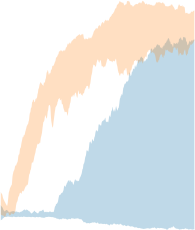
\includegraphics[interpolate=true,width=1.950000in,height=2.300000in]{shape-20-img2.png}}%
\end{pgfscope}%
\begin{pgfscope}%
\pgfsetbuttcap%
\pgfsetroundjoin%
\definecolor{currentfill}{rgb}{0.000000,0.000000,0.000000}%
\pgfsetfillcolor{currentfill}%
\pgfsetlinewidth{0.803000pt}%
\definecolor{currentstroke}{rgb}{0.000000,0.000000,0.000000}%
\pgfsetstrokecolor{currentstroke}%
\pgfsetdash{}{0pt}%
\pgfsys@defobject{currentmarker}{\pgfqpoint{0.000000in}{-0.048611in}}{\pgfqpoint{0.000000in}{0.000000in}}{%
\pgfpathmoveto{\pgfqpoint{0.000000in}{0.000000in}}%
\pgfpathlineto{\pgfqpoint{0.000000in}{-0.048611in}}%
\pgfusepath{stroke,fill}%
}%
\begin{pgfscope}%
\pgfsys@transformshift{3.437307in}{0.524170in}%
\pgfsys@useobject{currentmarker}{}%
\end{pgfscope}%
\end{pgfscope}%
\begin{pgfscope}%
\definecolor{textcolor}{rgb}{0.000000,0.000000,0.000000}%
\pgfsetstrokecolor{textcolor}%
\pgfsetfillcolor{textcolor}%
\pgftext[x=3.437307in,y=0.426948in,,top]{\color{textcolor}\rmfamily\fontsize{8.000000}{9.600000}\selectfont \(\displaystyle {0.0}\)}%
\end{pgfscope}%
\begin{pgfscope}%
\pgfsetbuttcap%
\pgfsetroundjoin%
\definecolor{currentfill}{rgb}{0.000000,0.000000,0.000000}%
\pgfsetfillcolor{currentfill}%
\pgfsetlinewidth{0.803000pt}%
\definecolor{currentstroke}{rgb}{0.000000,0.000000,0.000000}%
\pgfsetstrokecolor{currentstroke}%
\pgfsetdash{}{0pt}%
\pgfsys@defobject{currentmarker}{\pgfqpoint{0.000000in}{-0.048611in}}{\pgfqpoint{0.000000in}{0.000000in}}{%
\pgfpathmoveto{\pgfqpoint{0.000000in}{0.000000in}}%
\pgfpathlineto{\pgfqpoint{0.000000in}{-0.048611in}}%
\pgfusepath{stroke,fill}%
}%
\begin{pgfscope}%
\pgfsys@transformshift{3.829846in}{0.524170in}%
\pgfsys@useobject{currentmarker}{}%
\end{pgfscope}%
\end{pgfscope}%
\begin{pgfscope}%
\definecolor{textcolor}{rgb}{0.000000,0.000000,0.000000}%
\pgfsetstrokecolor{textcolor}%
\pgfsetfillcolor{textcolor}%
\pgftext[x=3.829846in,y=0.426948in,,top]{\color{textcolor}\rmfamily\fontsize{8.000000}{9.600000}\selectfont \(\displaystyle {0.5}\)}%
\end{pgfscope}%
\begin{pgfscope}%
\pgfsetbuttcap%
\pgfsetroundjoin%
\definecolor{currentfill}{rgb}{0.000000,0.000000,0.000000}%
\pgfsetfillcolor{currentfill}%
\pgfsetlinewidth{0.803000pt}%
\definecolor{currentstroke}{rgb}{0.000000,0.000000,0.000000}%
\pgfsetstrokecolor{currentstroke}%
\pgfsetdash{}{0pt}%
\pgfsys@defobject{currentmarker}{\pgfqpoint{0.000000in}{-0.048611in}}{\pgfqpoint{0.000000in}{0.000000in}}{%
\pgfpathmoveto{\pgfqpoint{0.000000in}{0.000000in}}%
\pgfpathlineto{\pgfqpoint{0.000000in}{-0.048611in}}%
\pgfusepath{stroke,fill}%
}%
\begin{pgfscope}%
\pgfsys@transformshift{4.222384in}{0.524170in}%
\pgfsys@useobject{currentmarker}{}%
\end{pgfscope}%
\end{pgfscope}%
\begin{pgfscope}%
\definecolor{textcolor}{rgb}{0.000000,0.000000,0.000000}%
\pgfsetstrokecolor{textcolor}%
\pgfsetfillcolor{textcolor}%
\pgftext[x=4.222384in,y=0.426948in,,top]{\color{textcolor}\rmfamily\fontsize{8.000000}{9.600000}\selectfont \(\displaystyle {1.0}\)}%
\end{pgfscope}%
\begin{pgfscope}%
\pgfsetbuttcap%
\pgfsetroundjoin%
\definecolor{currentfill}{rgb}{0.000000,0.000000,0.000000}%
\pgfsetfillcolor{currentfill}%
\pgfsetlinewidth{0.803000pt}%
\definecolor{currentstroke}{rgb}{0.000000,0.000000,0.000000}%
\pgfsetstrokecolor{currentstroke}%
\pgfsetdash{}{0pt}%
\pgfsys@defobject{currentmarker}{\pgfqpoint{0.000000in}{-0.048611in}}{\pgfqpoint{0.000000in}{0.000000in}}{%
\pgfpathmoveto{\pgfqpoint{0.000000in}{0.000000in}}%
\pgfpathlineto{\pgfqpoint{0.000000in}{-0.048611in}}%
\pgfusepath{stroke,fill}%
}%
\begin{pgfscope}%
\pgfsys@transformshift{4.614923in}{0.524170in}%
\pgfsys@useobject{currentmarker}{}%
\end{pgfscope}%
\end{pgfscope}%
\begin{pgfscope}%
\definecolor{textcolor}{rgb}{0.000000,0.000000,0.000000}%
\pgfsetstrokecolor{textcolor}%
\pgfsetfillcolor{textcolor}%
\pgftext[x=4.614923in,y=0.426948in,,top]{\color{textcolor}\rmfamily\fontsize{8.000000}{9.600000}\selectfont \(\displaystyle {1.5}\)}%
\end{pgfscope}%
\begin{pgfscope}%
\pgfsetbuttcap%
\pgfsetroundjoin%
\definecolor{currentfill}{rgb}{0.000000,0.000000,0.000000}%
\pgfsetfillcolor{currentfill}%
\pgfsetlinewidth{0.803000pt}%
\definecolor{currentstroke}{rgb}{0.000000,0.000000,0.000000}%
\pgfsetstrokecolor{currentstroke}%
\pgfsetdash{}{0pt}%
\pgfsys@defobject{currentmarker}{\pgfqpoint{0.000000in}{-0.048611in}}{\pgfqpoint{0.000000in}{0.000000in}}{%
\pgfpathmoveto{\pgfqpoint{0.000000in}{0.000000in}}%
\pgfpathlineto{\pgfqpoint{0.000000in}{-0.048611in}}%
\pgfusepath{stroke,fill}%
}%
\begin{pgfscope}%
\pgfsys@transformshift{5.007462in}{0.524170in}%
\pgfsys@useobject{currentmarker}{}%
\end{pgfscope}%
\end{pgfscope}%
\begin{pgfscope}%
\definecolor{textcolor}{rgb}{0.000000,0.000000,0.000000}%
\pgfsetstrokecolor{textcolor}%
\pgfsetfillcolor{textcolor}%
\pgftext[x=5.007462in,y=0.426948in,,top]{\color{textcolor}\rmfamily\fontsize{8.000000}{9.600000}\selectfont \(\displaystyle {2.0}\)}%
\end{pgfscope}%
\begin{pgfscope}%
\pgfsetbuttcap%
\pgfsetroundjoin%
\definecolor{currentfill}{rgb}{0.000000,0.000000,0.000000}%
\pgfsetfillcolor{currentfill}%
\pgfsetlinewidth{0.803000pt}%
\definecolor{currentstroke}{rgb}{0.000000,0.000000,0.000000}%
\pgfsetstrokecolor{currentstroke}%
\pgfsetdash{}{0pt}%
\pgfsys@defobject{currentmarker}{\pgfqpoint{0.000000in}{-0.048611in}}{\pgfqpoint{0.000000in}{0.000000in}}{%
\pgfpathmoveto{\pgfqpoint{0.000000in}{0.000000in}}%
\pgfpathlineto{\pgfqpoint{0.000000in}{-0.048611in}}%
\pgfusepath{stroke,fill}%
}%
\begin{pgfscope}%
\pgfsys@transformshift{5.400001in}{0.524170in}%
\pgfsys@useobject{currentmarker}{}%
\end{pgfscope}%
\end{pgfscope}%
\begin{pgfscope}%
\definecolor{textcolor}{rgb}{0.000000,0.000000,0.000000}%
\pgfsetstrokecolor{textcolor}%
\pgfsetfillcolor{textcolor}%
\pgftext[x=5.400001in,y=0.426948in,,top]{\color{textcolor}\rmfamily\fontsize{8.000000}{9.600000}\selectfont \(\displaystyle {2.5}\)}%
\end{pgfscope}%
\begin{pgfscope}%
\definecolor{textcolor}{rgb}{0.000000,0.000000,0.000000}%
\pgfsetstrokecolor{textcolor}%
\pgfsetfillcolor{textcolor}%
\pgftext[x=4.430889in,y=0.263862in,,top]{\color{textcolor}\rmfamily\fontsize{10.000000}{12.000000}\selectfont step}%
\end{pgfscope}%
\begin{pgfscope}%
\definecolor{textcolor}{rgb}{0.000000,0.000000,0.000000}%
\pgfsetstrokecolor{textcolor}%
\pgfsetfillcolor{textcolor}%
\pgftext[x=5.495496in,y=0.277751in,right,top]{\color{textcolor}\rmfamily\fontsize{8.000000}{9.600000}\selectfont \(\displaystyle \times{10^{7}}{}\)}%
\end{pgfscope}%
\begin{pgfscope}%
\pgfsetbuttcap%
\pgfsetroundjoin%
\definecolor{currentfill}{rgb}{0.000000,0.000000,0.000000}%
\pgfsetfillcolor{currentfill}%
\pgfsetlinewidth{0.803000pt}%
\definecolor{currentstroke}{rgb}{0.000000,0.000000,0.000000}%
\pgfsetstrokecolor{currentstroke}%
\pgfsetdash{}{0pt}%
\pgfsys@defobject{currentmarker}{\pgfqpoint{-0.048611in}{0.000000in}}{\pgfqpoint{-0.000000in}{0.000000in}}{%
\pgfpathmoveto{\pgfqpoint{-0.000000in}{0.000000in}}%
\pgfpathlineto{\pgfqpoint{-0.048611in}{0.000000in}}%
\pgfusepath{stroke,fill}%
}%
\begin{pgfscope}%
\pgfsys@transformshift{3.366281in}{0.756819in}%
\pgfsys@useobject{currentmarker}{}%
\end{pgfscope}%
\end{pgfscope}%
\begin{pgfscope}%
\definecolor{textcolor}{rgb}{0.000000,0.000000,0.000000}%
\pgfsetstrokecolor{textcolor}%
\pgfsetfillcolor{textcolor}%
\pgftext[x=3.118208in, y=0.714610in, left, base]{\color{textcolor}\rmfamily\fontsize{8.000000}{9.600000}\selectfont \(\displaystyle {0.0}\)}%
\end{pgfscope}%
\begin{pgfscope}%
\pgfsetbuttcap%
\pgfsetroundjoin%
\definecolor{currentfill}{rgb}{0.000000,0.000000,0.000000}%
\pgfsetfillcolor{currentfill}%
\pgfsetlinewidth{0.803000pt}%
\definecolor{currentstroke}{rgb}{0.000000,0.000000,0.000000}%
\pgfsetstrokecolor{currentstroke}%
\pgfsetdash{}{0pt}%
\pgfsys@defobject{currentmarker}{\pgfqpoint{-0.048611in}{0.000000in}}{\pgfqpoint{-0.000000in}{0.000000in}}{%
\pgfpathmoveto{\pgfqpoint{-0.000000in}{0.000000in}}%
\pgfpathlineto{\pgfqpoint{-0.048611in}{0.000000in}}%
\pgfusepath{stroke,fill}%
}%
\begin{pgfscope}%
\pgfsys@transformshift{3.366281in}{1.173231in}%
\pgfsys@useobject{currentmarker}{}%
\end{pgfscope}%
\end{pgfscope}%
\begin{pgfscope}%
\definecolor{textcolor}{rgb}{0.000000,0.000000,0.000000}%
\pgfsetstrokecolor{textcolor}%
\pgfsetfillcolor{textcolor}%
\pgftext[x=3.118208in, y=1.131022in, left, base]{\color{textcolor}\rmfamily\fontsize{8.000000}{9.600000}\selectfont \(\displaystyle {0.2}\)}%
\end{pgfscope}%
\begin{pgfscope}%
\pgfsetbuttcap%
\pgfsetroundjoin%
\definecolor{currentfill}{rgb}{0.000000,0.000000,0.000000}%
\pgfsetfillcolor{currentfill}%
\pgfsetlinewidth{0.803000pt}%
\definecolor{currentstroke}{rgb}{0.000000,0.000000,0.000000}%
\pgfsetstrokecolor{currentstroke}%
\pgfsetdash{}{0pt}%
\pgfsys@defobject{currentmarker}{\pgfqpoint{-0.048611in}{0.000000in}}{\pgfqpoint{-0.000000in}{0.000000in}}{%
\pgfpathmoveto{\pgfqpoint{-0.000000in}{0.000000in}}%
\pgfpathlineto{\pgfqpoint{-0.048611in}{0.000000in}}%
\pgfusepath{stroke,fill}%
}%
\begin{pgfscope}%
\pgfsys@transformshift{3.366281in}{1.589643in}%
\pgfsys@useobject{currentmarker}{}%
\end{pgfscope}%
\end{pgfscope}%
\begin{pgfscope}%
\definecolor{textcolor}{rgb}{0.000000,0.000000,0.000000}%
\pgfsetstrokecolor{textcolor}%
\pgfsetfillcolor{textcolor}%
\pgftext[x=3.118208in, y=1.547434in, left, base]{\color{textcolor}\rmfamily\fontsize{8.000000}{9.600000}\selectfont \(\displaystyle {0.4}\)}%
\end{pgfscope}%
\begin{pgfscope}%
\pgfsetbuttcap%
\pgfsetroundjoin%
\definecolor{currentfill}{rgb}{0.000000,0.000000,0.000000}%
\pgfsetfillcolor{currentfill}%
\pgfsetlinewidth{0.803000pt}%
\definecolor{currentstroke}{rgb}{0.000000,0.000000,0.000000}%
\pgfsetstrokecolor{currentstroke}%
\pgfsetdash{}{0pt}%
\pgfsys@defobject{currentmarker}{\pgfqpoint{-0.048611in}{0.000000in}}{\pgfqpoint{-0.000000in}{0.000000in}}{%
\pgfpathmoveto{\pgfqpoint{-0.000000in}{0.000000in}}%
\pgfpathlineto{\pgfqpoint{-0.048611in}{0.000000in}}%
\pgfusepath{stroke,fill}%
}%
\begin{pgfscope}%
\pgfsys@transformshift{3.366281in}{2.006055in}%
\pgfsys@useobject{currentmarker}{}%
\end{pgfscope}%
\end{pgfscope}%
\begin{pgfscope}%
\definecolor{textcolor}{rgb}{0.000000,0.000000,0.000000}%
\pgfsetstrokecolor{textcolor}%
\pgfsetfillcolor{textcolor}%
\pgftext[x=3.118208in, y=1.963846in, left, base]{\color{textcolor}\rmfamily\fontsize{8.000000}{9.600000}\selectfont \(\displaystyle {0.6}\)}%
\end{pgfscope}%
\begin{pgfscope}%
\pgfsetbuttcap%
\pgfsetroundjoin%
\definecolor{currentfill}{rgb}{0.000000,0.000000,0.000000}%
\pgfsetfillcolor{currentfill}%
\pgfsetlinewidth{0.803000pt}%
\definecolor{currentstroke}{rgb}{0.000000,0.000000,0.000000}%
\pgfsetstrokecolor{currentstroke}%
\pgfsetdash{}{0pt}%
\pgfsys@defobject{currentmarker}{\pgfqpoint{-0.048611in}{0.000000in}}{\pgfqpoint{-0.000000in}{0.000000in}}{%
\pgfpathmoveto{\pgfqpoint{-0.000000in}{0.000000in}}%
\pgfpathlineto{\pgfqpoint{-0.048611in}{0.000000in}}%
\pgfusepath{stroke,fill}%
}%
\begin{pgfscope}%
\pgfsys@transformshift{3.366281in}{2.422467in}%
\pgfsys@useobject{currentmarker}{}%
\end{pgfscope}%
\end{pgfscope}%
\begin{pgfscope}%
\definecolor{textcolor}{rgb}{0.000000,0.000000,0.000000}%
\pgfsetstrokecolor{textcolor}%
\pgfsetfillcolor{textcolor}%
\pgftext[x=3.118208in, y=2.380258in, left, base]{\color{textcolor}\rmfamily\fontsize{8.000000}{9.600000}\selectfont \(\displaystyle {0.8}\)}%
\end{pgfscope}%
\begin{pgfscope}%
\pgfsetbuttcap%
\pgfsetroundjoin%
\definecolor{currentfill}{rgb}{0.000000,0.000000,0.000000}%
\pgfsetfillcolor{currentfill}%
\pgfsetlinewidth{0.803000pt}%
\definecolor{currentstroke}{rgb}{0.000000,0.000000,0.000000}%
\pgfsetstrokecolor{currentstroke}%
\pgfsetdash{}{0pt}%
\pgfsys@defobject{currentmarker}{\pgfqpoint{-0.048611in}{0.000000in}}{\pgfqpoint{-0.000000in}{0.000000in}}{%
\pgfpathmoveto{\pgfqpoint{-0.000000in}{0.000000in}}%
\pgfpathlineto{\pgfqpoint{-0.048611in}{0.000000in}}%
\pgfusepath{stroke,fill}%
}%
\begin{pgfscope}%
\pgfsys@transformshift{3.366281in}{2.838879in}%
\pgfsys@useobject{currentmarker}{}%
\end{pgfscope}%
\end{pgfscope}%
\begin{pgfscope}%
\definecolor{textcolor}{rgb}{0.000000,0.000000,0.000000}%
\pgfsetstrokecolor{textcolor}%
\pgfsetfillcolor{textcolor}%
\pgftext[x=3.118208in, y=2.796670in, left, base]{\color{textcolor}\rmfamily\fontsize{8.000000}{9.600000}\selectfont \(\displaystyle {1.0}\)}%
\end{pgfscope}%
\begin{pgfscope}%
\definecolor{textcolor}{rgb}{0.000000,0.000000,0.000000}%
\pgfsetstrokecolor{textcolor}%
\pgfsetfillcolor{textcolor}%
\pgftext[x=3.062652in,y=1.782842in,,bottom,rotate=90.000000]{\color{textcolor}\rmfamily\fontsize{10.000000}{12.000000}\selectfont success}%
\end{pgfscope}%
\begin{pgfscope}%
\pgfsys@transformshift{3.440000in}{0.779108in}%
\pgftext[left,bottom]{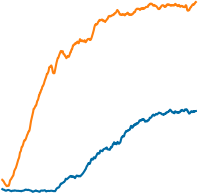
\includegraphics[interpolate=true,width=1.980000in,height=1.930000in]{shape-20-img3.png}}%
\end{pgfscope}%
\begin{pgfscope}%
\pgfsetrectcap%
\pgfsetmiterjoin%
\pgfsetlinewidth{0.803000pt}%
\definecolor{currentstroke}{rgb}{0.000000,0.000000,0.000000}%
\pgfsetstrokecolor{currentstroke}%
\pgfsetdash{}{0pt}%
\pgfpathmoveto{\pgfqpoint{3.366281in}{0.524170in}}%
\pgfpathlineto{\pgfqpoint{3.366281in}{3.041514in}}%
\pgfusepath{stroke}%
\end{pgfscope}%
\begin{pgfscope}%
\pgfsetrectcap%
\pgfsetmiterjoin%
\pgfsetlinewidth{0.803000pt}%
\definecolor{currentstroke}{rgb}{0.000000,0.000000,0.000000}%
\pgfsetstrokecolor{currentstroke}%
\pgfsetdash{}{0pt}%
\pgfpathmoveto{\pgfqpoint{5.495496in}{0.524170in}}%
\pgfpathlineto{\pgfqpoint{5.495496in}{3.041514in}}%
\pgfusepath{stroke}%
\end{pgfscope}%
\begin{pgfscope}%
\pgfsetrectcap%
\pgfsetmiterjoin%
\pgfsetlinewidth{0.803000pt}%
\definecolor{currentstroke}{rgb}{0.000000,0.000000,0.000000}%
\pgfsetstrokecolor{currentstroke}%
\pgfsetdash{}{0pt}%
\pgfpathmoveto{\pgfqpoint{3.366281in}{0.524170in}}%
\pgfpathlineto{\pgfqpoint{5.495496in}{0.524170in}}%
\pgfusepath{stroke}%
\end{pgfscope}%
\begin{pgfscope}%
\pgfsetrectcap%
\pgfsetmiterjoin%
\pgfsetlinewidth{0.803000pt}%
\definecolor{currentstroke}{rgb}{0.000000,0.000000,0.000000}%
\pgfsetstrokecolor{currentstroke}%
\pgfsetdash{}{0pt}%
\pgfpathmoveto{\pgfqpoint{3.366281in}{3.041514in}}%
\pgfpathlineto{\pgfqpoint{5.495496in}{3.041514in}}%
\pgfusepath{stroke}%
\end{pgfscope}%
\begin{pgfscope}%
\pgfsetrectcap%
\pgfsetroundjoin%
\pgfsetlinewidth{1.505625pt}%
\definecolor{currentstroke}{rgb}{0.000000,0.419608,0.643137}%
\pgfsetstrokecolor{currentstroke}%
\pgfsetdash{}{0pt}%
\pgfpathmoveto{\pgfqpoint{4.746603in}{1.872621in}}%
\pgfpathlineto{\pgfqpoint{4.857714in}{1.872621in}}%
\pgfpathlineto{\pgfqpoint{4.968825in}{1.872621in}}%
\pgfusepath{stroke}%
\end{pgfscope}%
\begin{pgfscope}%
\definecolor{textcolor}{rgb}{0.000000,0.000000,0.000000}%
\pgfsetstrokecolor{textcolor}%
\pgfsetfillcolor{textcolor}%
\pgftext[x=5.057714in,y=1.833732in,left,base]{\color{textcolor}\rmfamily\fontsize{8.000000}{9.600000}\selectfont LSTM}%
\end{pgfscope}%
\begin{pgfscope}%
\pgfsetrectcap%
\pgfsetroundjoin%
\pgfsetlinewidth{1.505625pt}%
\definecolor{currentstroke}{rgb}{1.000000,0.501961,0.054902}%
\pgfsetstrokecolor{currentstroke}%
\pgfsetdash{}{0pt}%
\pgfpathmoveto{\pgfqpoint{4.746603in}{1.709535in}}%
\pgfpathlineto{\pgfqpoint{4.857714in}{1.709535in}}%
\pgfpathlineto{\pgfqpoint{4.968825in}{1.709535in}}%
\pgfusepath{stroke}%
\end{pgfscope}%
\begin{pgfscope}%
\definecolor{textcolor}{rgb}{0.000000,0.000000,0.000000}%
\pgfsetstrokecolor{textcolor}%
\pgfsetfillcolor{textcolor}%
\pgftext[x=5.057714in,y=1.670646in,left,base]{\color{textcolor}\rmfamily\fontsize{8.000000}{9.600000}\selectfont MAP}%
\end{pgfscope}%
\begin{pgfscope}%
\definecolor{textcolor}{rgb}{0.000000,0.000000,0.000000}%
\pgfsetstrokecolor{textcolor}%
\pgfsetfillcolor{textcolor}%
\pgftext[x=2.822748in,y=3.419326in,,top]{\color{textcolor}\rmfamily\fontsize{12.000000}{14.400000}\selectfont \(\displaystyle 20 \times 20\) search space}%
\end{pgfscope}%
\end{pgfpicture}%
\makeatother%
\endgroup%

    \caption[Learning curves for different search space sizes.]{Episode length and success rate curves during training for three different search space sizes. Mean and standard deviation across 4 runs.}
    \label{fig:shape}
\end{figure}

\section{Number of Training Samples}
\label{sec:sample}

Figure~\ref{fig:sample} shows how the average length and success rate in the terrain environment is affected by the number of samples seen during training.
These metrics are presented for the limited training set and unlimited testing set respectively.

It seems like both architectures can overfit to training sets of as many as 1000 samples,
For smaller training set sizes, search path lengths on the test get gradually worse past a certain time step.
Interestingly the LSTM architecture seems to overfit more severely to small training sets.
Its performance on the test set decreases substantially past a certain time step.
The spatial memory architecture does not overfit as severely.
For both architectures, as many as 10000 training samples are needed to generalize to the full distribution of scenes and achieve the same performance on the training and test sets. 

\begin{figure}
    \centering
    \(500\) samples
    %% Creator: Matplotlib, PGF backend
%%
%% To include the figure in your LaTeX document, write
%%   \input{<filename>.pgf}
%%
%% Make sure the required packages are loaded in your preamble
%%   \usepackage{pgf}
%%
%% Also ensure that all the required font packages are loaded; for instance,
%% the lmodern package is sometimes necessary when using math font.
%%   \usepackage{lmodern}
%%
%% Figures using additional raster images can only be included by \input if
%% they are in the same directory as the main LaTeX file. For loading figures
%% from other directories you can use the `import` package
%%   \usepackage{import}
%%
%% and then include the figures with
%%   \import{<path to file>}{<filename>.pgf}
%%
%% Matplotlib used the following preamble
%%   \usepackage{fontspec}
%%   \setmainfont{DejaVuSerif.ttf}[Path=\detokenize{/home/oslund/Thesis/repo/venv/lib/python3.8/site-packages/matplotlib/mpl-data/fonts/ttf/}]
%%   \setsansfont{DejaVuSans.ttf}[Path=\detokenize{/home/oslund/Thesis/repo/venv/lib/python3.8/site-packages/matplotlib/mpl-data/fonts/ttf/}]
%%   \setmonofont{DejaVuSansMono.ttf}[Path=\detokenize{/home/oslund/Thesis/repo/venv/lib/python3.8/site-packages/matplotlib/mpl-data/fonts/ttf/}]
%%
\begingroup%
\makeatletter%
\begin{pgfpicture}%
\pgfpathrectangle{\pgfpointorigin}{\pgfqpoint{5.559542in}{1.896475in}}%
\pgfusepath{use as bounding box, clip}%
\begin{pgfscope}%
\pgfsetbuttcap%
\pgfsetmiterjoin%
\definecolor{currentfill}{rgb}{1.000000,1.000000,1.000000}%
\pgfsetfillcolor{currentfill}%
\pgfsetlinewidth{0.000000pt}%
\definecolor{currentstroke}{rgb}{1.000000,1.000000,1.000000}%
\pgfsetstrokecolor{currentstroke}%
\pgfsetstrokeopacity{0.000000}%
\pgfsetdash{}{0pt}%
\pgfpathmoveto{\pgfqpoint{0.000000in}{0.000000in}}%
\pgfpathlineto{\pgfqpoint{5.559542in}{0.000000in}}%
\pgfpathlineto{\pgfqpoint{5.559542in}{1.896475in}}%
\pgfpathlineto{\pgfqpoint{0.000000in}{1.896475in}}%
\pgfpathlineto{\pgfqpoint{0.000000in}{0.000000in}}%
\pgfpathclose%
\pgfusepath{fill}%
\end{pgfscope}%
\begin{pgfscope}%
\pgfsetbuttcap%
\pgfsetmiterjoin%
\definecolor{currentfill}{rgb}{1.000000,1.000000,1.000000}%
\pgfsetfillcolor{currentfill}%
\pgfsetlinewidth{0.000000pt}%
\definecolor{currentstroke}{rgb}{0.000000,0.000000,0.000000}%
\pgfsetstrokecolor{currentstroke}%
\pgfsetstrokeopacity{0.000000}%
\pgfsetdash{}{0pt}%
\pgfpathmoveto{\pgfqpoint{0.600965in}{0.529443in}}%
\pgfpathlineto{\pgfqpoint{2.724862in}{0.529443in}}%
\pgfpathlineto{\pgfqpoint{2.724862in}{1.796475in}}%
\pgfpathlineto{\pgfqpoint{0.600965in}{1.796475in}}%
\pgfpathlineto{\pgfqpoint{0.600965in}{0.529443in}}%
\pgfpathclose%
\pgfusepath{fill}%
\end{pgfscope}%
\begin{pgfscope}%
\pgfsetbuttcap%
\pgfsetroundjoin%
\definecolor{currentfill}{rgb}{0.150000,0.150000,0.150000}%
\pgfsetfillcolor{currentfill}%
\pgfsetlinewidth{1.254687pt}%
\definecolor{currentstroke}{rgb}{0.150000,0.150000,0.150000}%
\pgfsetstrokecolor{currentstroke}%
\pgfsetdash{}{0pt}%
\pgfsys@defobject{currentmarker}{\pgfqpoint{0.000000in}{-0.083333in}}{\pgfqpoint{0.000000in}{0.000000in}}{%
\pgfpathmoveto{\pgfqpoint{0.000000in}{0.000000in}}%
\pgfpathlineto{\pgfqpoint{0.000000in}{-0.083333in}}%
\pgfusepath{stroke,fill}%
}%
\begin{pgfscope}%
\pgfsys@transformshift{0.658075in}{0.529443in}%
\pgfsys@useobject{currentmarker}{}%
\end{pgfscope}%
\end{pgfscope}%
\begin{pgfscope}%
\definecolor{textcolor}{rgb}{0.150000,0.150000,0.150000}%
\pgfsetstrokecolor{textcolor}%
\pgfsetfillcolor{textcolor}%
\pgftext[x=0.658075in,y=0.397499in,,top]{\color{textcolor}\rmfamily\fontsize{8.000000}{9.600000}\selectfont \(\displaystyle {0.0}\)}%
\end{pgfscope}%
\begin{pgfscope}%
\pgfsetbuttcap%
\pgfsetroundjoin%
\definecolor{currentfill}{rgb}{0.150000,0.150000,0.150000}%
\pgfsetfillcolor{currentfill}%
\pgfsetlinewidth{1.254687pt}%
\definecolor{currentstroke}{rgb}{0.150000,0.150000,0.150000}%
\pgfsetstrokecolor{currentstroke}%
\pgfsetdash{}{0pt}%
\pgfsys@defobject{currentmarker}{\pgfqpoint{0.000000in}{-0.083333in}}{\pgfqpoint{0.000000in}{0.000000in}}{%
\pgfpathmoveto{\pgfqpoint{0.000000in}{0.000000in}}%
\pgfpathlineto{\pgfqpoint{0.000000in}{-0.083333in}}%
\pgfusepath{stroke,fill}%
}%
\begin{pgfscope}%
\pgfsys@transformshift{1.052383in}{0.529443in}%
\pgfsys@useobject{currentmarker}{}%
\end{pgfscope}%
\end{pgfscope}%
\begin{pgfscope}%
\definecolor{textcolor}{rgb}{0.150000,0.150000,0.150000}%
\pgfsetstrokecolor{textcolor}%
\pgfsetfillcolor{textcolor}%
\pgftext[x=1.052383in,y=0.397499in,,top]{\color{textcolor}\rmfamily\fontsize{8.000000}{9.600000}\selectfont \(\displaystyle {0.5}\)}%
\end{pgfscope}%
\begin{pgfscope}%
\pgfsetbuttcap%
\pgfsetroundjoin%
\definecolor{currentfill}{rgb}{0.150000,0.150000,0.150000}%
\pgfsetfillcolor{currentfill}%
\pgfsetlinewidth{1.254687pt}%
\definecolor{currentstroke}{rgb}{0.150000,0.150000,0.150000}%
\pgfsetstrokecolor{currentstroke}%
\pgfsetdash{}{0pt}%
\pgfsys@defobject{currentmarker}{\pgfqpoint{0.000000in}{-0.083333in}}{\pgfqpoint{0.000000in}{0.000000in}}{%
\pgfpathmoveto{\pgfqpoint{0.000000in}{0.000000in}}%
\pgfpathlineto{\pgfqpoint{0.000000in}{-0.083333in}}%
\pgfusepath{stroke,fill}%
}%
\begin{pgfscope}%
\pgfsys@transformshift{1.446691in}{0.529443in}%
\pgfsys@useobject{currentmarker}{}%
\end{pgfscope}%
\end{pgfscope}%
\begin{pgfscope}%
\definecolor{textcolor}{rgb}{0.150000,0.150000,0.150000}%
\pgfsetstrokecolor{textcolor}%
\pgfsetfillcolor{textcolor}%
\pgftext[x=1.446691in,y=0.397499in,,top]{\color{textcolor}\rmfamily\fontsize{8.000000}{9.600000}\selectfont \(\displaystyle {1.0}\)}%
\end{pgfscope}%
\begin{pgfscope}%
\pgfsetbuttcap%
\pgfsetroundjoin%
\definecolor{currentfill}{rgb}{0.150000,0.150000,0.150000}%
\pgfsetfillcolor{currentfill}%
\pgfsetlinewidth{1.254687pt}%
\definecolor{currentstroke}{rgb}{0.150000,0.150000,0.150000}%
\pgfsetstrokecolor{currentstroke}%
\pgfsetdash{}{0pt}%
\pgfsys@defobject{currentmarker}{\pgfqpoint{0.000000in}{-0.083333in}}{\pgfqpoint{0.000000in}{0.000000in}}{%
\pgfpathmoveto{\pgfqpoint{0.000000in}{0.000000in}}%
\pgfpathlineto{\pgfqpoint{0.000000in}{-0.083333in}}%
\pgfusepath{stroke,fill}%
}%
\begin{pgfscope}%
\pgfsys@transformshift{1.840999in}{0.529443in}%
\pgfsys@useobject{currentmarker}{}%
\end{pgfscope}%
\end{pgfscope}%
\begin{pgfscope}%
\definecolor{textcolor}{rgb}{0.150000,0.150000,0.150000}%
\pgfsetstrokecolor{textcolor}%
\pgfsetfillcolor{textcolor}%
\pgftext[x=1.840999in,y=0.397499in,,top]{\color{textcolor}\rmfamily\fontsize{8.000000}{9.600000}\selectfont \(\displaystyle {1.5}\)}%
\end{pgfscope}%
\begin{pgfscope}%
\pgfsetbuttcap%
\pgfsetroundjoin%
\definecolor{currentfill}{rgb}{0.150000,0.150000,0.150000}%
\pgfsetfillcolor{currentfill}%
\pgfsetlinewidth{1.254687pt}%
\definecolor{currentstroke}{rgb}{0.150000,0.150000,0.150000}%
\pgfsetstrokecolor{currentstroke}%
\pgfsetdash{}{0pt}%
\pgfsys@defobject{currentmarker}{\pgfqpoint{0.000000in}{-0.083333in}}{\pgfqpoint{0.000000in}{0.000000in}}{%
\pgfpathmoveto{\pgfqpoint{0.000000in}{0.000000in}}%
\pgfpathlineto{\pgfqpoint{0.000000in}{-0.083333in}}%
\pgfusepath{stroke,fill}%
}%
\begin{pgfscope}%
\pgfsys@transformshift{2.235306in}{0.529443in}%
\pgfsys@useobject{currentmarker}{}%
\end{pgfscope}%
\end{pgfscope}%
\begin{pgfscope}%
\definecolor{textcolor}{rgb}{0.150000,0.150000,0.150000}%
\pgfsetstrokecolor{textcolor}%
\pgfsetfillcolor{textcolor}%
\pgftext[x=2.235306in,y=0.397499in,,top]{\color{textcolor}\rmfamily\fontsize{8.000000}{9.600000}\selectfont \(\displaystyle {2.0}\)}%
\end{pgfscope}%
\begin{pgfscope}%
\pgfsetbuttcap%
\pgfsetroundjoin%
\definecolor{currentfill}{rgb}{0.150000,0.150000,0.150000}%
\pgfsetfillcolor{currentfill}%
\pgfsetlinewidth{1.254687pt}%
\definecolor{currentstroke}{rgb}{0.150000,0.150000,0.150000}%
\pgfsetstrokecolor{currentstroke}%
\pgfsetdash{}{0pt}%
\pgfsys@defobject{currentmarker}{\pgfqpoint{0.000000in}{-0.083333in}}{\pgfqpoint{0.000000in}{0.000000in}}{%
\pgfpathmoveto{\pgfqpoint{0.000000in}{0.000000in}}%
\pgfpathlineto{\pgfqpoint{0.000000in}{-0.083333in}}%
\pgfusepath{stroke,fill}%
}%
\begin{pgfscope}%
\pgfsys@transformshift{2.629614in}{0.529443in}%
\pgfsys@useobject{currentmarker}{}%
\end{pgfscope}%
\end{pgfscope}%
\begin{pgfscope}%
\definecolor{textcolor}{rgb}{0.150000,0.150000,0.150000}%
\pgfsetstrokecolor{textcolor}%
\pgfsetfillcolor{textcolor}%
\pgftext[x=2.629614in,y=0.397499in,,top]{\color{textcolor}\rmfamily\fontsize{8.000000}{9.600000}\selectfont \(\displaystyle {2.5}\)}%
\end{pgfscope}%
\begin{pgfscope}%
\definecolor{textcolor}{rgb}{0.150000,0.150000,0.150000}%
\pgfsetstrokecolor{textcolor}%
\pgfsetfillcolor{textcolor}%
\pgftext[x=1.662914in,y=0.234413in,,top]{\color{textcolor}\rmfamily\fontsize{10.000000}{12.000000}\selectfont step}%
\end{pgfscope}%
\begin{pgfscope}%
\definecolor{textcolor}{rgb}{0.150000,0.150000,0.150000}%
\pgfsetstrokecolor{textcolor}%
\pgfsetfillcolor{textcolor}%
\pgftext[x=2.724862in,y=0.248302in,right,top]{\color{textcolor}\rmfamily\fontsize{8.000000}{9.600000}\selectfont \(\displaystyle \times{10^{7}}{}\)}%
\end{pgfscope}%
\begin{pgfscope}%
\pgfsetbuttcap%
\pgfsetroundjoin%
\definecolor{currentfill}{rgb}{0.150000,0.150000,0.150000}%
\pgfsetfillcolor{currentfill}%
\pgfsetlinewidth{1.254687pt}%
\definecolor{currentstroke}{rgb}{0.150000,0.150000,0.150000}%
\pgfsetstrokecolor{currentstroke}%
\pgfsetdash{}{0pt}%
\pgfsys@defobject{currentmarker}{\pgfqpoint{-0.083333in}{0.000000in}}{\pgfqpoint{-0.000000in}{0.000000in}}{%
\pgfpathmoveto{\pgfqpoint{-0.000000in}{0.000000in}}%
\pgfpathlineto{\pgfqpoint{-0.083333in}{0.000000in}}%
\pgfusepath{stroke,fill}%
}%
\begin{pgfscope}%
\pgfsys@transformshift{0.600965in}{0.555116in}%
\pgfsys@useobject{currentmarker}{}%
\end{pgfscope}%
\end{pgfscope}%
\begin{pgfscope}%
\definecolor{textcolor}{rgb}{0.150000,0.150000,0.150000}%
\pgfsetstrokecolor{textcolor}%
\pgfsetfillcolor{textcolor}%
\pgftext[x=0.409992in, y=0.512907in, left, base]{\color{textcolor}\rmfamily\fontsize{8.000000}{9.600000}\selectfont \(\displaystyle {0}\)}%
\end{pgfscope}%
\begin{pgfscope}%
\pgfsetbuttcap%
\pgfsetroundjoin%
\definecolor{currentfill}{rgb}{0.150000,0.150000,0.150000}%
\pgfsetfillcolor{currentfill}%
\pgfsetlinewidth{1.254687pt}%
\definecolor{currentstroke}{rgb}{0.150000,0.150000,0.150000}%
\pgfsetstrokecolor{currentstroke}%
\pgfsetdash{}{0pt}%
\pgfsys@defobject{currentmarker}{\pgfqpoint{-0.083333in}{0.000000in}}{\pgfqpoint{-0.000000in}{0.000000in}}{%
\pgfpathmoveto{\pgfqpoint{-0.000000in}{0.000000in}}%
\pgfpathlineto{\pgfqpoint{-0.083333in}{0.000000in}}%
\pgfusepath{stroke,fill}%
}%
\begin{pgfscope}%
\pgfsys@transformshift{0.600965in}{0.853090in}%
\pgfsys@useobject{currentmarker}{}%
\end{pgfscope}%
\end{pgfscope}%
\begin{pgfscope}%
\definecolor{textcolor}{rgb}{0.150000,0.150000,0.150000}%
\pgfsetstrokecolor{textcolor}%
\pgfsetfillcolor{textcolor}%
\pgftext[x=0.291935in, y=0.810880in, left, base]{\color{textcolor}\rmfamily\fontsize{8.000000}{9.600000}\selectfont \(\displaystyle {200}\)}%
\end{pgfscope}%
\begin{pgfscope}%
\pgfsetbuttcap%
\pgfsetroundjoin%
\definecolor{currentfill}{rgb}{0.150000,0.150000,0.150000}%
\pgfsetfillcolor{currentfill}%
\pgfsetlinewidth{1.254687pt}%
\definecolor{currentstroke}{rgb}{0.150000,0.150000,0.150000}%
\pgfsetstrokecolor{currentstroke}%
\pgfsetdash{}{0pt}%
\pgfsys@defobject{currentmarker}{\pgfqpoint{-0.083333in}{0.000000in}}{\pgfqpoint{-0.000000in}{0.000000in}}{%
\pgfpathmoveto{\pgfqpoint{-0.000000in}{0.000000in}}%
\pgfpathlineto{\pgfqpoint{-0.083333in}{0.000000in}}%
\pgfusepath{stroke,fill}%
}%
\begin{pgfscope}%
\pgfsys@transformshift{0.600965in}{1.151063in}%
\pgfsys@useobject{currentmarker}{}%
\end{pgfscope}%
\end{pgfscope}%
\begin{pgfscope}%
\definecolor{textcolor}{rgb}{0.150000,0.150000,0.150000}%
\pgfsetstrokecolor{textcolor}%
\pgfsetfillcolor{textcolor}%
\pgftext[x=0.291935in, y=1.108854in, left, base]{\color{textcolor}\rmfamily\fontsize{8.000000}{9.600000}\selectfont \(\displaystyle {400}\)}%
\end{pgfscope}%
\begin{pgfscope}%
\pgfsetbuttcap%
\pgfsetroundjoin%
\definecolor{currentfill}{rgb}{0.150000,0.150000,0.150000}%
\pgfsetfillcolor{currentfill}%
\pgfsetlinewidth{1.254687pt}%
\definecolor{currentstroke}{rgb}{0.150000,0.150000,0.150000}%
\pgfsetstrokecolor{currentstroke}%
\pgfsetdash{}{0pt}%
\pgfsys@defobject{currentmarker}{\pgfqpoint{-0.083333in}{0.000000in}}{\pgfqpoint{-0.000000in}{0.000000in}}{%
\pgfpathmoveto{\pgfqpoint{-0.000000in}{0.000000in}}%
\pgfpathlineto{\pgfqpoint{-0.083333in}{0.000000in}}%
\pgfusepath{stroke,fill}%
}%
\begin{pgfscope}%
\pgfsys@transformshift{0.600965in}{1.449036in}%
\pgfsys@useobject{currentmarker}{}%
\end{pgfscope}%
\end{pgfscope}%
\begin{pgfscope}%
\definecolor{textcolor}{rgb}{0.150000,0.150000,0.150000}%
\pgfsetstrokecolor{textcolor}%
\pgfsetfillcolor{textcolor}%
\pgftext[x=0.291935in, y=1.406827in, left, base]{\color{textcolor}\rmfamily\fontsize{8.000000}{9.600000}\selectfont \(\displaystyle {600}\)}%
\end{pgfscope}%
\begin{pgfscope}%
\pgfsetbuttcap%
\pgfsetroundjoin%
\definecolor{currentfill}{rgb}{0.150000,0.150000,0.150000}%
\pgfsetfillcolor{currentfill}%
\pgfsetlinewidth{1.254687pt}%
\definecolor{currentstroke}{rgb}{0.150000,0.150000,0.150000}%
\pgfsetstrokecolor{currentstroke}%
\pgfsetdash{}{0pt}%
\pgfsys@defobject{currentmarker}{\pgfqpoint{-0.083333in}{0.000000in}}{\pgfqpoint{-0.000000in}{0.000000in}}{%
\pgfpathmoveto{\pgfqpoint{-0.000000in}{0.000000in}}%
\pgfpathlineto{\pgfqpoint{-0.083333in}{0.000000in}}%
\pgfusepath{stroke,fill}%
}%
\begin{pgfscope}%
\pgfsys@transformshift{0.600965in}{1.747010in}%
\pgfsys@useobject{currentmarker}{}%
\end{pgfscope}%
\end{pgfscope}%
\begin{pgfscope}%
\definecolor{textcolor}{rgb}{0.150000,0.150000,0.150000}%
\pgfsetstrokecolor{textcolor}%
\pgfsetfillcolor{textcolor}%
\pgftext[x=0.291935in, y=1.704801in, left, base]{\color{textcolor}\rmfamily\fontsize{8.000000}{9.600000}\selectfont \(\displaystyle {800}\)}%
\end{pgfscope}%
\begin{pgfscope}%
\definecolor{textcolor}{rgb}{0.150000,0.150000,0.150000}%
\pgfsetstrokecolor{textcolor}%
\pgfsetfillcolor{textcolor}%
\pgftext[x=0.236379in,y=1.162959in,,bottom,rotate=90.000000]{\color{textcolor}\rmfamily\fontsize{10.000000}{12.000000}\selectfont length}%
\end{pgfscope}%
\begin{pgfscope}%
\pgfsys@transformshift{0.680556in}{0.577030in}%
\pgftext[left,bottom]{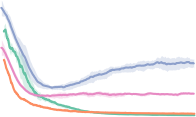
\includegraphics[interpolate=true,width=1.958333in,height=1.166667in]{sample-500-img0.png}}%
\end{pgfscope}%
\begin{pgfscope}%
\pgfsetrectcap%
\pgfsetmiterjoin%
\pgfsetlinewidth{1.254687pt}%
\definecolor{currentstroke}{rgb}{0.150000,0.150000,0.150000}%
\pgfsetstrokecolor{currentstroke}%
\pgfsetdash{}{0pt}%
\pgfpathmoveto{\pgfqpoint{0.600965in}{0.529443in}}%
\pgfpathlineto{\pgfqpoint{0.600965in}{1.796475in}}%
\pgfusepath{stroke}%
\end{pgfscope}%
\begin{pgfscope}%
\pgfsetrectcap%
\pgfsetmiterjoin%
\pgfsetlinewidth{1.254687pt}%
\definecolor{currentstroke}{rgb}{0.150000,0.150000,0.150000}%
\pgfsetstrokecolor{currentstroke}%
\pgfsetdash{}{0pt}%
\pgfpathmoveto{\pgfqpoint{2.724862in}{0.529443in}}%
\pgfpathlineto{\pgfqpoint{2.724862in}{1.796475in}}%
\pgfusepath{stroke}%
\end{pgfscope}%
\begin{pgfscope}%
\pgfsetrectcap%
\pgfsetmiterjoin%
\pgfsetlinewidth{1.254687pt}%
\definecolor{currentstroke}{rgb}{0.150000,0.150000,0.150000}%
\pgfsetstrokecolor{currentstroke}%
\pgfsetdash{}{0pt}%
\pgfpathmoveto{\pgfqpoint{0.600965in}{0.529443in}}%
\pgfpathlineto{\pgfqpoint{2.724862in}{0.529443in}}%
\pgfusepath{stroke}%
\end{pgfscope}%
\begin{pgfscope}%
\pgfsetrectcap%
\pgfsetmiterjoin%
\pgfsetlinewidth{1.254687pt}%
\definecolor{currentstroke}{rgb}{0.150000,0.150000,0.150000}%
\pgfsetstrokecolor{currentstroke}%
\pgfsetdash{}{0pt}%
\pgfpathmoveto{\pgfqpoint{0.600965in}{1.796475in}}%
\pgfpathlineto{\pgfqpoint{2.724862in}{1.796475in}}%
\pgfusepath{stroke}%
\end{pgfscope}%
\begin{pgfscope}%
\pgfsetbuttcap%
\pgfsetmiterjoin%
\definecolor{currentfill}{rgb}{1.000000,1.000000,1.000000}%
\pgfsetfillcolor{currentfill}%
\pgfsetlinewidth{0.000000pt}%
\definecolor{currentstroke}{rgb}{0.000000,0.000000,0.000000}%
\pgfsetstrokecolor{currentstroke}%
\pgfsetstrokeopacity{0.000000}%
\pgfsetdash{}{0pt}%
\pgfpathmoveto{\pgfqpoint{3.335645in}{0.529443in}}%
\pgfpathlineto{\pgfqpoint{5.459542in}{0.529443in}}%
\pgfpathlineto{\pgfqpoint{5.459542in}{1.796475in}}%
\pgfpathlineto{\pgfqpoint{3.335645in}{1.796475in}}%
\pgfpathlineto{\pgfqpoint{3.335645in}{0.529443in}}%
\pgfpathclose%
\pgfusepath{fill}%
\end{pgfscope}%
\begin{pgfscope}%
\pgfsetbuttcap%
\pgfsetroundjoin%
\definecolor{currentfill}{rgb}{0.150000,0.150000,0.150000}%
\pgfsetfillcolor{currentfill}%
\pgfsetlinewidth{1.254687pt}%
\definecolor{currentstroke}{rgb}{0.150000,0.150000,0.150000}%
\pgfsetstrokecolor{currentstroke}%
\pgfsetdash{}{0pt}%
\pgfsys@defobject{currentmarker}{\pgfqpoint{0.000000in}{-0.083333in}}{\pgfqpoint{0.000000in}{0.000000in}}{%
\pgfpathmoveto{\pgfqpoint{0.000000in}{0.000000in}}%
\pgfpathlineto{\pgfqpoint{0.000000in}{-0.083333in}}%
\pgfusepath{stroke,fill}%
}%
\begin{pgfscope}%
\pgfsys@transformshift{3.392755in}{0.529443in}%
\pgfsys@useobject{currentmarker}{}%
\end{pgfscope}%
\end{pgfscope}%
\begin{pgfscope}%
\definecolor{textcolor}{rgb}{0.150000,0.150000,0.150000}%
\pgfsetstrokecolor{textcolor}%
\pgfsetfillcolor{textcolor}%
\pgftext[x=3.392755in,y=0.397499in,,top]{\color{textcolor}\rmfamily\fontsize{8.000000}{9.600000}\selectfont \(\displaystyle {0.0}\)}%
\end{pgfscope}%
\begin{pgfscope}%
\pgfsetbuttcap%
\pgfsetroundjoin%
\definecolor{currentfill}{rgb}{0.150000,0.150000,0.150000}%
\pgfsetfillcolor{currentfill}%
\pgfsetlinewidth{1.254687pt}%
\definecolor{currentstroke}{rgb}{0.150000,0.150000,0.150000}%
\pgfsetstrokecolor{currentstroke}%
\pgfsetdash{}{0pt}%
\pgfsys@defobject{currentmarker}{\pgfqpoint{0.000000in}{-0.083333in}}{\pgfqpoint{0.000000in}{0.000000in}}{%
\pgfpathmoveto{\pgfqpoint{0.000000in}{0.000000in}}%
\pgfpathlineto{\pgfqpoint{0.000000in}{-0.083333in}}%
\pgfusepath{stroke,fill}%
}%
\begin{pgfscope}%
\pgfsys@transformshift{3.787063in}{0.529443in}%
\pgfsys@useobject{currentmarker}{}%
\end{pgfscope}%
\end{pgfscope}%
\begin{pgfscope}%
\definecolor{textcolor}{rgb}{0.150000,0.150000,0.150000}%
\pgfsetstrokecolor{textcolor}%
\pgfsetfillcolor{textcolor}%
\pgftext[x=3.787063in,y=0.397499in,,top]{\color{textcolor}\rmfamily\fontsize{8.000000}{9.600000}\selectfont \(\displaystyle {0.5}\)}%
\end{pgfscope}%
\begin{pgfscope}%
\pgfsetbuttcap%
\pgfsetroundjoin%
\definecolor{currentfill}{rgb}{0.150000,0.150000,0.150000}%
\pgfsetfillcolor{currentfill}%
\pgfsetlinewidth{1.254687pt}%
\definecolor{currentstroke}{rgb}{0.150000,0.150000,0.150000}%
\pgfsetstrokecolor{currentstroke}%
\pgfsetdash{}{0pt}%
\pgfsys@defobject{currentmarker}{\pgfqpoint{0.000000in}{-0.083333in}}{\pgfqpoint{0.000000in}{0.000000in}}{%
\pgfpathmoveto{\pgfqpoint{0.000000in}{0.000000in}}%
\pgfpathlineto{\pgfqpoint{0.000000in}{-0.083333in}}%
\pgfusepath{stroke,fill}%
}%
\begin{pgfscope}%
\pgfsys@transformshift{4.181370in}{0.529443in}%
\pgfsys@useobject{currentmarker}{}%
\end{pgfscope}%
\end{pgfscope}%
\begin{pgfscope}%
\definecolor{textcolor}{rgb}{0.150000,0.150000,0.150000}%
\pgfsetstrokecolor{textcolor}%
\pgfsetfillcolor{textcolor}%
\pgftext[x=4.181370in,y=0.397499in,,top]{\color{textcolor}\rmfamily\fontsize{8.000000}{9.600000}\selectfont \(\displaystyle {1.0}\)}%
\end{pgfscope}%
\begin{pgfscope}%
\pgfsetbuttcap%
\pgfsetroundjoin%
\definecolor{currentfill}{rgb}{0.150000,0.150000,0.150000}%
\pgfsetfillcolor{currentfill}%
\pgfsetlinewidth{1.254687pt}%
\definecolor{currentstroke}{rgb}{0.150000,0.150000,0.150000}%
\pgfsetstrokecolor{currentstroke}%
\pgfsetdash{}{0pt}%
\pgfsys@defobject{currentmarker}{\pgfqpoint{0.000000in}{-0.083333in}}{\pgfqpoint{0.000000in}{0.000000in}}{%
\pgfpathmoveto{\pgfqpoint{0.000000in}{0.000000in}}%
\pgfpathlineto{\pgfqpoint{0.000000in}{-0.083333in}}%
\pgfusepath{stroke,fill}%
}%
\begin{pgfscope}%
\pgfsys@transformshift{4.575678in}{0.529443in}%
\pgfsys@useobject{currentmarker}{}%
\end{pgfscope}%
\end{pgfscope}%
\begin{pgfscope}%
\definecolor{textcolor}{rgb}{0.150000,0.150000,0.150000}%
\pgfsetstrokecolor{textcolor}%
\pgfsetfillcolor{textcolor}%
\pgftext[x=4.575678in,y=0.397499in,,top]{\color{textcolor}\rmfamily\fontsize{8.000000}{9.600000}\selectfont \(\displaystyle {1.5}\)}%
\end{pgfscope}%
\begin{pgfscope}%
\pgfsetbuttcap%
\pgfsetroundjoin%
\definecolor{currentfill}{rgb}{0.150000,0.150000,0.150000}%
\pgfsetfillcolor{currentfill}%
\pgfsetlinewidth{1.254687pt}%
\definecolor{currentstroke}{rgb}{0.150000,0.150000,0.150000}%
\pgfsetstrokecolor{currentstroke}%
\pgfsetdash{}{0pt}%
\pgfsys@defobject{currentmarker}{\pgfqpoint{0.000000in}{-0.083333in}}{\pgfqpoint{0.000000in}{0.000000in}}{%
\pgfpathmoveto{\pgfqpoint{0.000000in}{0.000000in}}%
\pgfpathlineto{\pgfqpoint{0.000000in}{-0.083333in}}%
\pgfusepath{stroke,fill}%
}%
\begin{pgfscope}%
\pgfsys@transformshift{4.969986in}{0.529443in}%
\pgfsys@useobject{currentmarker}{}%
\end{pgfscope}%
\end{pgfscope}%
\begin{pgfscope}%
\definecolor{textcolor}{rgb}{0.150000,0.150000,0.150000}%
\pgfsetstrokecolor{textcolor}%
\pgfsetfillcolor{textcolor}%
\pgftext[x=4.969986in,y=0.397499in,,top]{\color{textcolor}\rmfamily\fontsize{8.000000}{9.600000}\selectfont \(\displaystyle {2.0}\)}%
\end{pgfscope}%
\begin{pgfscope}%
\pgfsetbuttcap%
\pgfsetroundjoin%
\definecolor{currentfill}{rgb}{0.150000,0.150000,0.150000}%
\pgfsetfillcolor{currentfill}%
\pgfsetlinewidth{1.254687pt}%
\definecolor{currentstroke}{rgb}{0.150000,0.150000,0.150000}%
\pgfsetstrokecolor{currentstroke}%
\pgfsetdash{}{0pt}%
\pgfsys@defobject{currentmarker}{\pgfqpoint{0.000000in}{-0.083333in}}{\pgfqpoint{0.000000in}{0.000000in}}{%
\pgfpathmoveto{\pgfqpoint{0.000000in}{0.000000in}}%
\pgfpathlineto{\pgfqpoint{0.000000in}{-0.083333in}}%
\pgfusepath{stroke,fill}%
}%
\begin{pgfscope}%
\pgfsys@transformshift{5.364294in}{0.529443in}%
\pgfsys@useobject{currentmarker}{}%
\end{pgfscope}%
\end{pgfscope}%
\begin{pgfscope}%
\definecolor{textcolor}{rgb}{0.150000,0.150000,0.150000}%
\pgfsetstrokecolor{textcolor}%
\pgfsetfillcolor{textcolor}%
\pgftext[x=5.364294in,y=0.397499in,,top]{\color{textcolor}\rmfamily\fontsize{8.000000}{9.600000}\selectfont \(\displaystyle {2.5}\)}%
\end{pgfscope}%
\begin{pgfscope}%
\definecolor{textcolor}{rgb}{0.150000,0.150000,0.150000}%
\pgfsetstrokecolor{textcolor}%
\pgfsetfillcolor{textcolor}%
\pgftext[x=4.397593in,y=0.234413in,,top]{\color{textcolor}\rmfamily\fontsize{10.000000}{12.000000}\selectfont step}%
\end{pgfscope}%
\begin{pgfscope}%
\definecolor{textcolor}{rgb}{0.150000,0.150000,0.150000}%
\pgfsetstrokecolor{textcolor}%
\pgfsetfillcolor{textcolor}%
\pgftext[x=5.459542in,y=0.248302in,right,top]{\color{textcolor}\rmfamily\fontsize{8.000000}{9.600000}\selectfont \(\displaystyle \times{10^{7}}{}\)}%
\end{pgfscope}%
\begin{pgfscope}%
\pgfsetbuttcap%
\pgfsetroundjoin%
\definecolor{currentfill}{rgb}{0.150000,0.150000,0.150000}%
\pgfsetfillcolor{currentfill}%
\pgfsetlinewidth{1.254687pt}%
\definecolor{currentstroke}{rgb}{0.150000,0.150000,0.150000}%
\pgfsetstrokecolor{currentstroke}%
\pgfsetdash{}{0pt}%
\pgfsys@defobject{currentmarker}{\pgfqpoint{-0.083333in}{0.000000in}}{\pgfqpoint{-0.000000in}{0.000000in}}{%
\pgfpathmoveto{\pgfqpoint{-0.000000in}{0.000000in}}%
\pgfpathlineto{\pgfqpoint{-0.083333in}{0.000000in}}%
\pgfusepath{stroke,fill}%
}%
\begin{pgfscope}%
\pgfsys@transformshift{3.335645in}{0.653140in}%
\pgfsys@useobject{currentmarker}{}%
\end{pgfscope}%
\end{pgfscope}%
\begin{pgfscope}%
\definecolor{textcolor}{rgb}{0.150000,0.150000,0.150000}%
\pgfsetstrokecolor{textcolor}%
\pgfsetfillcolor{textcolor}%
\pgftext[x=3.052849in, y=0.610930in, left, base]{\color{textcolor}\rmfamily\fontsize{8.000000}{9.600000}\selectfont \(\displaystyle {0.4}\)}%
\end{pgfscope}%
\begin{pgfscope}%
\pgfsetbuttcap%
\pgfsetroundjoin%
\definecolor{currentfill}{rgb}{0.150000,0.150000,0.150000}%
\pgfsetfillcolor{currentfill}%
\pgfsetlinewidth{1.254687pt}%
\definecolor{currentstroke}{rgb}{0.150000,0.150000,0.150000}%
\pgfsetstrokecolor{currentstroke}%
\pgfsetdash{}{0pt}%
\pgfsys@defobject{currentmarker}{\pgfqpoint{-0.083333in}{0.000000in}}{\pgfqpoint{-0.000000in}{0.000000in}}{%
\pgfpathmoveto{\pgfqpoint{-0.000000in}{0.000000in}}%
\pgfpathlineto{\pgfqpoint{-0.083333in}{0.000000in}}%
\pgfusepath{stroke,fill}%
}%
\begin{pgfscope}%
\pgfsys@transformshift{3.335645in}{1.014365in}%
\pgfsys@useobject{currentmarker}{}%
\end{pgfscope}%
\end{pgfscope}%
\begin{pgfscope}%
\definecolor{textcolor}{rgb}{0.150000,0.150000,0.150000}%
\pgfsetstrokecolor{textcolor}%
\pgfsetfillcolor{textcolor}%
\pgftext[x=3.052849in, y=0.972156in, left, base]{\color{textcolor}\rmfamily\fontsize{8.000000}{9.600000}\selectfont \(\displaystyle {0.6}\)}%
\end{pgfscope}%
\begin{pgfscope}%
\pgfsetbuttcap%
\pgfsetroundjoin%
\definecolor{currentfill}{rgb}{0.150000,0.150000,0.150000}%
\pgfsetfillcolor{currentfill}%
\pgfsetlinewidth{1.254687pt}%
\definecolor{currentstroke}{rgb}{0.150000,0.150000,0.150000}%
\pgfsetstrokecolor{currentstroke}%
\pgfsetdash{}{0pt}%
\pgfsys@defobject{currentmarker}{\pgfqpoint{-0.083333in}{0.000000in}}{\pgfqpoint{-0.000000in}{0.000000in}}{%
\pgfpathmoveto{\pgfqpoint{-0.000000in}{0.000000in}}%
\pgfpathlineto{\pgfqpoint{-0.083333in}{0.000000in}}%
\pgfusepath{stroke,fill}%
}%
\begin{pgfscope}%
\pgfsys@transformshift{3.335645in}{1.375591in}%
\pgfsys@useobject{currentmarker}{}%
\end{pgfscope}%
\end{pgfscope}%
\begin{pgfscope}%
\definecolor{textcolor}{rgb}{0.150000,0.150000,0.150000}%
\pgfsetstrokecolor{textcolor}%
\pgfsetfillcolor{textcolor}%
\pgftext[x=3.052849in, y=1.333382in, left, base]{\color{textcolor}\rmfamily\fontsize{8.000000}{9.600000}\selectfont \(\displaystyle {0.8}\)}%
\end{pgfscope}%
\begin{pgfscope}%
\pgfsetbuttcap%
\pgfsetroundjoin%
\definecolor{currentfill}{rgb}{0.150000,0.150000,0.150000}%
\pgfsetfillcolor{currentfill}%
\pgfsetlinewidth{1.254687pt}%
\definecolor{currentstroke}{rgb}{0.150000,0.150000,0.150000}%
\pgfsetstrokecolor{currentstroke}%
\pgfsetdash{}{0pt}%
\pgfsys@defobject{currentmarker}{\pgfqpoint{-0.083333in}{0.000000in}}{\pgfqpoint{-0.000000in}{0.000000in}}{%
\pgfpathmoveto{\pgfqpoint{-0.000000in}{0.000000in}}%
\pgfpathlineto{\pgfqpoint{-0.083333in}{0.000000in}}%
\pgfusepath{stroke,fill}%
}%
\begin{pgfscope}%
\pgfsys@transformshift{3.335645in}{1.736817in}%
\pgfsys@useobject{currentmarker}{}%
\end{pgfscope}%
\end{pgfscope}%
\begin{pgfscope}%
\definecolor{textcolor}{rgb}{0.150000,0.150000,0.150000}%
\pgfsetstrokecolor{textcolor}%
\pgfsetfillcolor{textcolor}%
\pgftext[x=3.052849in, y=1.694607in, left, base]{\color{textcolor}\rmfamily\fontsize{8.000000}{9.600000}\selectfont \(\displaystyle {1.0}\)}%
\end{pgfscope}%
\begin{pgfscope}%
\definecolor{textcolor}{rgb}{0.150000,0.150000,0.150000}%
\pgfsetstrokecolor{textcolor}%
\pgfsetfillcolor{textcolor}%
\pgftext[x=2.997294in,y=1.162959in,,bottom,rotate=90.000000]{\color{textcolor}\rmfamily\fontsize{10.000000}{12.000000}\selectfont success}%
\end{pgfscope}%
\begin{pgfscope}%
\pgfsys@transformshift{3.416667in}{0.590919in}%
\pgftext[left,bottom]{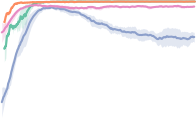
\includegraphics[interpolate=true,width=1.958333in,height=1.166667in]{sample-500-img1.png}}%
\end{pgfscope}%
\begin{pgfscope}%
\pgfsetrectcap%
\pgfsetmiterjoin%
\pgfsetlinewidth{1.254687pt}%
\definecolor{currentstroke}{rgb}{0.150000,0.150000,0.150000}%
\pgfsetstrokecolor{currentstroke}%
\pgfsetdash{}{0pt}%
\pgfpathmoveto{\pgfqpoint{3.335645in}{0.529443in}}%
\pgfpathlineto{\pgfqpoint{3.335645in}{1.796475in}}%
\pgfusepath{stroke}%
\end{pgfscope}%
\begin{pgfscope}%
\pgfsetrectcap%
\pgfsetmiterjoin%
\pgfsetlinewidth{1.254687pt}%
\definecolor{currentstroke}{rgb}{0.150000,0.150000,0.150000}%
\pgfsetstrokecolor{currentstroke}%
\pgfsetdash{}{0pt}%
\pgfpathmoveto{\pgfqpoint{5.459542in}{0.529443in}}%
\pgfpathlineto{\pgfqpoint{5.459542in}{1.796475in}}%
\pgfusepath{stroke}%
\end{pgfscope}%
\begin{pgfscope}%
\pgfsetrectcap%
\pgfsetmiterjoin%
\pgfsetlinewidth{1.254687pt}%
\definecolor{currentstroke}{rgb}{0.150000,0.150000,0.150000}%
\pgfsetstrokecolor{currentstroke}%
\pgfsetdash{}{0pt}%
\pgfpathmoveto{\pgfqpoint{3.335645in}{0.529443in}}%
\pgfpathlineto{\pgfqpoint{5.459542in}{0.529443in}}%
\pgfusepath{stroke}%
\end{pgfscope}%
\begin{pgfscope}%
\pgfsetrectcap%
\pgfsetmiterjoin%
\pgfsetlinewidth{1.254687pt}%
\definecolor{currentstroke}{rgb}{0.150000,0.150000,0.150000}%
\pgfsetstrokecolor{currentstroke}%
\pgfsetdash{}{0pt}%
\pgfpathmoveto{\pgfqpoint{3.335645in}{1.796475in}}%
\pgfpathlineto{\pgfqpoint{5.459542in}{1.796475in}}%
\pgfusepath{stroke}%
\end{pgfscope}%
\end{pgfpicture}%
\makeatother%
\endgroup%

    \(1000\) samples
    %% Creator: Matplotlib, PGF backend
%%
%% To include the figure in your LaTeX document, write
%%   \input{<filename>.pgf}
%%
%% Make sure the required packages are loaded in your preamble
%%   \usepackage{pgf}
%%
%% Also ensure that all the required font packages are loaded; for instance,
%% the lmodern package is sometimes necessary when using math font.
%%   \usepackage{lmodern}
%%
%% Figures using additional raster images can only be included by \input if
%% they are in the same directory as the main LaTeX file. For loading figures
%% from other directories you can use the `import` package
%%   \usepackage{import}
%%
%% and then include the figures with
%%   \import{<path to file>}{<filename>.pgf}
%%
%% Matplotlib used the following preamble
%%   \usepackage{fontspec}
%%   \setmainfont{DejaVuSerif.ttf}[Path=\detokenize{/home/oslund/.local/lib/python3.8/site-packages/matplotlib/mpl-data/fonts/ttf/}]
%%   \setsansfont{DejaVuSans.ttf}[Path=\detokenize{/home/oslund/.local/lib/python3.8/site-packages/matplotlib/mpl-data/fonts/ttf/}]
%%   \setmonofont{DejaVuSansMono.ttf}[Path=\detokenize{/home/oslund/.local/lib/python3.8/site-packages/matplotlib/mpl-data/fonts/ttf/}]
%%
\begingroup%
\makeatletter%
\begin{pgfpicture}%
\pgfpathrectangle{\pgfpointorigin}{\pgfqpoint{5.645496in}{2.822748in}}%
\pgfusepath{use as bounding box, clip}%
\begin{pgfscope}%
\pgfsetbuttcap%
\pgfsetmiterjoin%
\definecolor{currentfill}{rgb}{1.000000,1.000000,1.000000}%
\pgfsetfillcolor{currentfill}%
\pgfsetlinewidth{0.000000pt}%
\definecolor{currentstroke}{rgb}{1.000000,1.000000,1.000000}%
\pgfsetstrokecolor{currentstroke}%
\pgfsetdash{}{0pt}%
\pgfpathmoveto{\pgfqpoint{0.000000in}{0.000000in}}%
\pgfpathlineto{\pgfqpoint{5.645496in}{0.000000in}}%
\pgfpathlineto{\pgfqpoint{5.645496in}{2.822748in}}%
\pgfpathlineto{\pgfqpoint{0.000000in}{2.822748in}}%
\pgfpathlineto{\pgfqpoint{0.000000in}{0.000000in}}%
\pgfpathclose%
\pgfusepath{fill}%
\end{pgfscope}%
\begin{pgfscope}%
\pgfsetbuttcap%
\pgfsetmiterjoin%
\definecolor{currentfill}{rgb}{1.000000,1.000000,1.000000}%
\pgfsetfillcolor{currentfill}%
\pgfsetlinewidth{0.000000pt}%
\definecolor{currentstroke}{rgb}{0.000000,0.000000,0.000000}%
\pgfsetstrokecolor{currentstroke}%
\pgfsetstrokeopacity{0.000000}%
\pgfsetdash{}{0pt}%
\pgfpathmoveto{\pgfqpoint{0.636920in}{0.558892in}}%
\pgfpathlineto{\pgfqpoint{2.731412in}{0.558892in}}%
\pgfpathlineto{\pgfqpoint{2.731412in}{2.375154in}}%
\pgfpathlineto{\pgfqpoint{0.636920in}{2.375154in}}%
\pgfpathlineto{\pgfqpoint{0.636920in}{0.558892in}}%
\pgfpathclose%
\pgfusepath{fill}%
\end{pgfscope}%
\begin{pgfscope}%
\pgfsetbuttcap%
\pgfsetroundjoin%
\definecolor{currentfill}{rgb}{0.150000,0.150000,0.150000}%
\pgfsetfillcolor{currentfill}%
\pgfsetlinewidth{1.254687pt}%
\definecolor{currentstroke}{rgb}{0.150000,0.150000,0.150000}%
\pgfsetstrokecolor{currentstroke}%
\pgfsetdash{}{0pt}%
\pgfsys@defobject{currentmarker}{\pgfqpoint{0.000000in}{-0.083333in}}{\pgfqpoint{0.000000in}{0.000000in}}{%
\pgfpathmoveto{\pgfqpoint{0.000000in}{0.000000in}}%
\pgfpathlineto{\pgfqpoint{0.000000in}{-0.083333in}}%
\pgfusepath{stroke,fill}%
}%
\begin{pgfscope}%
\pgfsys@transformshift{0.693239in}{0.558892in}%
\pgfsys@useobject{currentmarker}{}%
\end{pgfscope}%
\end{pgfscope}%
\begin{pgfscope}%
\definecolor{textcolor}{rgb}{0.150000,0.150000,0.150000}%
\pgfsetstrokecolor{textcolor}%
\pgfsetfillcolor{textcolor}%
\pgftext[x=0.693239in,y=0.426948in,,top]{\color{textcolor}\rmfamily\fontsize{8.000000}{9.600000}\selectfont \(\displaystyle {0.0}\)}%
\end{pgfscope}%
\begin{pgfscope}%
\pgfsetbuttcap%
\pgfsetroundjoin%
\definecolor{currentfill}{rgb}{0.150000,0.150000,0.150000}%
\pgfsetfillcolor{currentfill}%
\pgfsetlinewidth{1.254687pt}%
\definecolor{currentstroke}{rgb}{0.150000,0.150000,0.150000}%
\pgfsetstrokecolor{currentstroke}%
\pgfsetdash{}{0pt}%
\pgfsys@defobject{currentmarker}{\pgfqpoint{0.000000in}{-0.083333in}}{\pgfqpoint{0.000000in}{0.000000in}}{%
\pgfpathmoveto{\pgfqpoint{0.000000in}{0.000000in}}%
\pgfpathlineto{\pgfqpoint{0.000000in}{-0.083333in}}%
\pgfusepath{stroke,fill}%
}%
\begin{pgfscope}%
\pgfsys@transformshift{1.082088in}{0.558892in}%
\pgfsys@useobject{currentmarker}{}%
\end{pgfscope}%
\end{pgfscope}%
\begin{pgfscope}%
\definecolor{textcolor}{rgb}{0.150000,0.150000,0.150000}%
\pgfsetstrokecolor{textcolor}%
\pgfsetfillcolor{textcolor}%
\pgftext[x=1.082088in,y=0.426948in,,top]{\color{textcolor}\rmfamily\fontsize{8.000000}{9.600000}\selectfont \(\displaystyle {0.5}\)}%
\end{pgfscope}%
\begin{pgfscope}%
\pgfsetbuttcap%
\pgfsetroundjoin%
\definecolor{currentfill}{rgb}{0.150000,0.150000,0.150000}%
\pgfsetfillcolor{currentfill}%
\pgfsetlinewidth{1.254687pt}%
\definecolor{currentstroke}{rgb}{0.150000,0.150000,0.150000}%
\pgfsetstrokecolor{currentstroke}%
\pgfsetdash{}{0pt}%
\pgfsys@defobject{currentmarker}{\pgfqpoint{0.000000in}{-0.083333in}}{\pgfqpoint{0.000000in}{0.000000in}}{%
\pgfpathmoveto{\pgfqpoint{0.000000in}{0.000000in}}%
\pgfpathlineto{\pgfqpoint{0.000000in}{-0.083333in}}%
\pgfusepath{stroke,fill}%
}%
\begin{pgfscope}%
\pgfsys@transformshift{1.470937in}{0.558892in}%
\pgfsys@useobject{currentmarker}{}%
\end{pgfscope}%
\end{pgfscope}%
\begin{pgfscope}%
\definecolor{textcolor}{rgb}{0.150000,0.150000,0.150000}%
\pgfsetstrokecolor{textcolor}%
\pgfsetfillcolor{textcolor}%
\pgftext[x=1.470937in,y=0.426948in,,top]{\color{textcolor}\rmfamily\fontsize{8.000000}{9.600000}\selectfont \(\displaystyle {1.0}\)}%
\end{pgfscope}%
\begin{pgfscope}%
\pgfsetbuttcap%
\pgfsetroundjoin%
\definecolor{currentfill}{rgb}{0.150000,0.150000,0.150000}%
\pgfsetfillcolor{currentfill}%
\pgfsetlinewidth{1.254687pt}%
\definecolor{currentstroke}{rgb}{0.150000,0.150000,0.150000}%
\pgfsetstrokecolor{currentstroke}%
\pgfsetdash{}{0pt}%
\pgfsys@defobject{currentmarker}{\pgfqpoint{0.000000in}{-0.083333in}}{\pgfqpoint{0.000000in}{0.000000in}}{%
\pgfpathmoveto{\pgfqpoint{0.000000in}{0.000000in}}%
\pgfpathlineto{\pgfqpoint{0.000000in}{-0.083333in}}%
\pgfusepath{stroke,fill}%
}%
\begin{pgfscope}%
\pgfsys@transformshift{1.859786in}{0.558892in}%
\pgfsys@useobject{currentmarker}{}%
\end{pgfscope}%
\end{pgfscope}%
\begin{pgfscope}%
\definecolor{textcolor}{rgb}{0.150000,0.150000,0.150000}%
\pgfsetstrokecolor{textcolor}%
\pgfsetfillcolor{textcolor}%
\pgftext[x=1.859786in,y=0.426948in,,top]{\color{textcolor}\rmfamily\fontsize{8.000000}{9.600000}\selectfont \(\displaystyle {1.5}\)}%
\end{pgfscope}%
\begin{pgfscope}%
\pgfsetbuttcap%
\pgfsetroundjoin%
\definecolor{currentfill}{rgb}{0.150000,0.150000,0.150000}%
\pgfsetfillcolor{currentfill}%
\pgfsetlinewidth{1.254687pt}%
\definecolor{currentstroke}{rgb}{0.150000,0.150000,0.150000}%
\pgfsetstrokecolor{currentstroke}%
\pgfsetdash{}{0pt}%
\pgfsys@defobject{currentmarker}{\pgfqpoint{0.000000in}{-0.083333in}}{\pgfqpoint{0.000000in}{0.000000in}}{%
\pgfpathmoveto{\pgfqpoint{0.000000in}{0.000000in}}%
\pgfpathlineto{\pgfqpoint{0.000000in}{-0.083333in}}%
\pgfusepath{stroke,fill}%
}%
\begin{pgfscope}%
\pgfsys@transformshift{2.248634in}{0.558892in}%
\pgfsys@useobject{currentmarker}{}%
\end{pgfscope}%
\end{pgfscope}%
\begin{pgfscope}%
\definecolor{textcolor}{rgb}{0.150000,0.150000,0.150000}%
\pgfsetstrokecolor{textcolor}%
\pgfsetfillcolor{textcolor}%
\pgftext[x=2.248634in,y=0.426948in,,top]{\color{textcolor}\rmfamily\fontsize{8.000000}{9.600000}\selectfont \(\displaystyle {2.0}\)}%
\end{pgfscope}%
\begin{pgfscope}%
\pgfsetbuttcap%
\pgfsetroundjoin%
\definecolor{currentfill}{rgb}{0.150000,0.150000,0.150000}%
\pgfsetfillcolor{currentfill}%
\pgfsetlinewidth{1.254687pt}%
\definecolor{currentstroke}{rgb}{0.150000,0.150000,0.150000}%
\pgfsetstrokecolor{currentstroke}%
\pgfsetdash{}{0pt}%
\pgfsys@defobject{currentmarker}{\pgfqpoint{0.000000in}{-0.083333in}}{\pgfqpoint{0.000000in}{0.000000in}}{%
\pgfpathmoveto{\pgfqpoint{0.000000in}{0.000000in}}%
\pgfpathlineto{\pgfqpoint{0.000000in}{-0.083333in}}%
\pgfusepath{stroke,fill}%
}%
\begin{pgfscope}%
\pgfsys@transformshift{2.637483in}{0.558892in}%
\pgfsys@useobject{currentmarker}{}%
\end{pgfscope}%
\end{pgfscope}%
\begin{pgfscope}%
\definecolor{textcolor}{rgb}{0.150000,0.150000,0.150000}%
\pgfsetstrokecolor{textcolor}%
\pgfsetfillcolor{textcolor}%
\pgftext[x=2.637483in,y=0.426948in,,top]{\color{textcolor}\rmfamily\fontsize{8.000000}{9.600000}\selectfont \(\displaystyle {2.5}\)}%
\end{pgfscope}%
\begin{pgfscope}%
\definecolor{textcolor}{rgb}{0.150000,0.150000,0.150000}%
\pgfsetstrokecolor{textcolor}%
\pgfsetfillcolor{textcolor}%
\pgftext[x=1.684166in,y=0.263862in,,top]{\color{textcolor}\rmfamily\fontsize{10.000000}{12.000000}\selectfont step}%
\end{pgfscope}%
\begin{pgfscope}%
\definecolor{textcolor}{rgb}{0.150000,0.150000,0.150000}%
\pgfsetstrokecolor{textcolor}%
\pgfsetfillcolor{textcolor}%
\pgftext[x=2.731412in,y=0.277751in,right,top]{\color{textcolor}\rmfamily\fontsize{8.000000}{9.600000}\selectfont \(\displaystyle \times{10^{7}}{}\)}%
\end{pgfscope}%
\begin{pgfscope}%
\pgfsetbuttcap%
\pgfsetroundjoin%
\definecolor{currentfill}{rgb}{0.150000,0.150000,0.150000}%
\pgfsetfillcolor{currentfill}%
\pgfsetlinewidth{1.254687pt}%
\definecolor{currentstroke}{rgb}{0.150000,0.150000,0.150000}%
\pgfsetstrokecolor{currentstroke}%
\pgfsetdash{}{0pt}%
\pgfsys@defobject{currentmarker}{\pgfqpoint{-0.083333in}{0.000000in}}{\pgfqpoint{-0.000000in}{0.000000in}}{%
\pgfpathmoveto{\pgfqpoint{-0.000000in}{0.000000in}}%
\pgfpathlineto{\pgfqpoint{-0.083333in}{0.000000in}}%
\pgfusepath{stroke,fill}%
}%
\begin{pgfscope}%
\pgfsys@transformshift{0.636920in}{0.820885in}%
\pgfsys@useobject{currentmarker}{}%
\end{pgfscope}%
\end{pgfscope}%
\begin{pgfscope}%
\definecolor{textcolor}{rgb}{0.150000,0.150000,0.150000}%
\pgfsetstrokecolor{textcolor}%
\pgfsetfillcolor{textcolor}%
\pgftext[x=0.327890in, y=0.778675in, left, base]{\color{textcolor}\rmfamily\fontsize{8.000000}{9.600000}\selectfont \(\displaystyle {100}\)}%
\end{pgfscope}%
\begin{pgfscope}%
\pgfsetbuttcap%
\pgfsetroundjoin%
\definecolor{currentfill}{rgb}{0.150000,0.150000,0.150000}%
\pgfsetfillcolor{currentfill}%
\pgfsetlinewidth{1.254687pt}%
\definecolor{currentstroke}{rgb}{0.150000,0.150000,0.150000}%
\pgfsetstrokecolor{currentstroke}%
\pgfsetdash{}{0pt}%
\pgfsys@defobject{currentmarker}{\pgfqpoint{-0.083333in}{0.000000in}}{\pgfqpoint{-0.000000in}{0.000000in}}{%
\pgfpathmoveto{\pgfqpoint{-0.000000in}{0.000000in}}%
\pgfpathlineto{\pgfqpoint{-0.083333in}{0.000000in}}%
\pgfusepath{stroke,fill}%
}%
\begin{pgfscope}%
\pgfsys@transformshift{0.636920in}{1.139613in}%
\pgfsys@useobject{currentmarker}{}%
\end{pgfscope}%
\end{pgfscope}%
\begin{pgfscope}%
\definecolor{textcolor}{rgb}{0.150000,0.150000,0.150000}%
\pgfsetstrokecolor{textcolor}%
\pgfsetfillcolor{textcolor}%
\pgftext[x=0.327890in, y=1.097404in, left, base]{\color{textcolor}\rmfamily\fontsize{8.000000}{9.600000}\selectfont \(\displaystyle {200}\)}%
\end{pgfscope}%
\begin{pgfscope}%
\pgfsetbuttcap%
\pgfsetroundjoin%
\definecolor{currentfill}{rgb}{0.150000,0.150000,0.150000}%
\pgfsetfillcolor{currentfill}%
\pgfsetlinewidth{1.254687pt}%
\definecolor{currentstroke}{rgb}{0.150000,0.150000,0.150000}%
\pgfsetstrokecolor{currentstroke}%
\pgfsetdash{}{0pt}%
\pgfsys@defobject{currentmarker}{\pgfqpoint{-0.083333in}{0.000000in}}{\pgfqpoint{-0.000000in}{0.000000in}}{%
\pgfpathmoveto{\pgfqpoint{-0.000000in}{0.000000in}}%
\pgfpathlineto{\pgfqpoint{-0.083333in}{0.000000in}}%
\pgfusepath{stroke,fill}%
}%
\begin{pgfscope}%
\pgfsys@transformshift{0.636920in}{1.458342in}%
\pgfsys@useobject{currentmarker}{}%
\end{pgfscope}%
\end{pgfscope}%
\begin{pgfscope}%
\definecolor{textcolor}{rgb}{0.150000,0.150000,0.150000}%
\pgfsetstrokecolor{textcolor}%
\pgfsetfillcolor{textcolor}%
\pgftext[x=0.327890in, y=1.416132in, left, base]{\color{textcolor}\rmfamily\fontsize{8.000000}{9.600000}\selectfont \(\displaystyle {300}\)}%
\end{pgfscope}%
\begin{pgfscope}%
\pgfsetbuttcap%
\pgfsetroundjoin%
\definecolor{currentfill}{rgb}{0.150000,0.150000,0.150000}%
\pgfsetfillcolor{currentfill}%
\pgfsetlinewidth{1.254687pt}%
\definecolor{currentstroke}{rgb}{0.150000,0.150000,0.150000}%
\pgfsetstrokecolor{currentstroke}%
\pgfsetdash{}{0pt}%
\pgfsys@defobject{currentmarker}{\pgfqpoint{-0.083333in}{0.000000in}}{\pgfqpoint{-0.000000in}{0.000000in}}{%
\pgfpathmoveto{\pgfqpoint{-0.000000in}{0.000000in}}%
\pgfpathlineto{\pgfqpoint{-0.083333in}{0.000000in}}%
\pgfusepath{stroke,fill}%
}%
\begin{pgfscope}%
\pgfsys@transformshift{0.636920in}{1.777070in}%
\pgfsys@useobject{currentmarker}{}%
\end{pgfscope}%
\end{pgfscope}%
\begin{pgfscope}%
\definecolor{textcolor}{rgb}{0.150000,0.150000,0.150000}%
\pgfsetstrokecolor{textcolor}%
\pgfsetfillcolor{textcolor}%
\pgftext[x=0.327890in, y=1.734861in, left, base]{\color{textcolor}\rmfamily\fontsize{8.000000}{9.600000}\selectfont \(\displaystyle {400}\)}%
\end{pgfscope}%
\begin{pgfscope}%
\pgfsetbuttcap%
\pgfsetroundjoin%
\definecolor{currentfill}{rgb}{0.150000,0.150000,0.150000}%
\pgfsetfillcolor{currentfill}%
\pgfsetlinewidth{1.254687pt}%
\definecolor{currentstroke}{rgb}{0.150000,0.150000,0.150000}%
\pgfsetstrokecolor{currentstroke}%
\pgfsetdash{}{0pt}%
\pgfsys@defobject{currentmarker}{\pgfqpoint{-0.083333in}{0.000000in}}{\pgfqpoint{-0.000000in}{0.000000in}}{%
\pgfpathmoveto{\pgfqpoint{-0.000000in}{0.000000in}}%
\pgfpathlineto{\pgfqpoint{-0.083333in}{0.000000in}}%
\pgfusepath{stroke,fill}%
}%
\begin{pgfscope}%
\pgfsys@transformshift{0.636920in}{2.095799in}%
\pgfsys@useobject{currentmarker}{}%
\end{pgfscope}%
\end{pgfscope}%
\begin{pgfscope}%
\definecolor{textcolor}{rgb}{0.150000,0.150000,0.150000}%
\pgfsetstrokecolor{textcolor}%
\pgfsetfillcolor{textcolor}%
\pgftext[x=0.327890in, y=2.053589in, left, base]{\color{textcolor}\rmfamily\fontsize{8.000000}{9.600000}\selectfont \(\displaystyle {500}\)}%
\end{pgfscope}%
\begin{pgfscope}%
\definecolor{textcolor}{rgb}{0.150000,0.150000,0.150000}%
\pgfsetstrokecolor{textcolor}%
\pgfsetfillcolor{textcolor}%
\pgftext[x=0.272334in,y=1.467023in,,bottom,rotate=90.000000]{\color{textcolor}\rmfamily\fontsize{10.000000}{12.000000}\selectfont length}%
\end{pgfscope}%
\begin{pgfscope}%
\pgfsys@transformshift{0.720000in}{0.632748in}%
\pgftext[left,bottom]{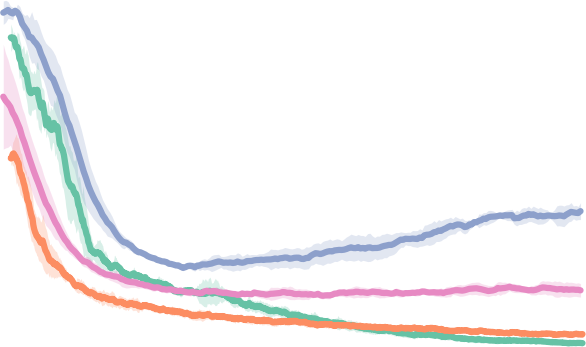
\includegraphics[interpolate=true,width=1.930000in,height=1.660000in]{sample-1000-img0.png}}%
\end{pgfscope}%
\begin{pgfscope}%
\pgfsetrectcap%
\pgfsetmiterjoin%
\pgfsetlinewidth{1.254687pt}%
\definecolor{currentstroke}{rgb}{0.150000,0.150000,0.150000}%
\pgfsetstrokecolor{currentstroke}%
\pgfsetdash{}{0pt}%
\pgfpathmoveto{\pgfqpoint{0.636920in}{0.558892in}}%
\pgfpathlineto{\pgfqpoint{0.636920in}{2.375154in}}%
\pgfusepath{stroke}%
\end{pgfscope}%
\begin{pgfscope}%
\pgfsetrectcap%
\pgfsetmiterjoin%
\pgfsetlinewidth{1.254687pt}%
\definecolor{currentstroke}{rgb}{0.150000,0.150000,0.150000}%
\pgfsetstrokecolor{currentstroke}%
\pgfsetdash{}{0pt}%
\pgfpathmoveto{\pgfqpoint{2.731412in}{0.558892in}}%
\pgfpathlineto{\pgfqpoint{2.731412in}{2.375154in}}%
\pgfusepath{stroke}%
\end{pgfscope}%
\begin{pgfscope}%
\pgfsetrectcap%
\pgfsetmiterjoin%
\pgfsetlinewidth{1.254687pt}%
\definecolor{currentstroke}{rgb}{0.150000,0.150000,0.150000}%
\pgfsetstrokecolor{currentstroke}%
\pgfsetdash{}{0pt}%
\pgfpathmoveto{\pgfqpoint{0.636920in}{0.558892in}}%
\pgfpathlineto{\pgfqpoint{2.731412in}{0.558892in}}%
\pgfusepath{stroke}%
\end{pgfscope}%
\begin{pgfscope}%
\pgfsetrectcap%
\pgfsetmiterjoin%
\pgfsetlinewidth{1.254687pt}%
\definecolor{currentstroke}{rgb}{0.150000,0.150000,0.150000}%
\pgfsetstrokecolor{currentstroke}%
\pgfsetdash{}{0pt}%
\pgfpathmoveto{\pgfqpoint{0.636920in}{2.375154in}}%
\pgfpathlineto{\pgfqpoint{2.731412in}{2.375154in}}%
\pgfusepath{stroke}%
\end{pgfscope}%
\begin{pgfscope}%
\pgfsetroundcap%
\pgfsetroundjoin%
\pgfsetlinewidth{1.505625pt}%
\definecolor{currentstroke}{rgb}{0.400000,0.760784,0.647059}%
\pgfsetstrokecolor{currentstroke}%
\pgfsetdash{}{0pt}%
\pgfpathmoveto{\pgfqpoint{1.745106in}{2.229624in}}%
\pgfpathlineto{\pgfqpoint{1.856217in}{2.229624in}}%
\pgfpathlineto{\pgfqpoint{1.967328in}{2.229624in}}%
\pgfusepath{stroke}%
\end{pgfscope}%
\begin{pgfscope}%
\definecolor{textcolor}{rgb}{0.150000,0.150000,0.150000}%
\pgfsetstrokecolor{textcolor}%
\pgfsetfillcolor{textcolor}%
\pgftext[x=2.056217in,y=2.190735in,left,base]{\color{textcolor}\rmfamily\fontsize{8.000000}{9.600000}\selectfont MAP train}%
\end{pgfscope}%
\begin{pgfscope}%
\pgfsetroundcap%
\pgfsetroundjoin%
\pgfsetlinewidth{1.505625pt}%
\definecolor{currentstroke}{rgb}{0.988235,0.552941,0.384314}%
\pgfsetstrokecolor{currentstroke}%
\pgfsetdash{}{0pt}%
\pgfpathmoveto{\pgfqpoint{1.745106in}{2.066539in}}%
\pgfpathlineto{\pgfqpoint{1.856217in}{2.066539in}}%
\pgfpathlineto{\pgfqpoint{1.967328in}{2.066539in}}%
\pgfusepath{stroke}%
\end{pgfscope}%
\begin{pgfscope}%
\definecolor{textcolor}{rgb}{0.150000,0.150000,0.150000}%
\pgfsetstrokecolor{textcolor}%
\pgfsetfillcolor{textcolor}%
\pgftext[x=2.056217in,y=2.027650in,left,base]{\color{textcolor}\rmfamily\fontsize{8.000000}{9.600000}\selectfont MAP test}%
\end{pgfscope}%
\begin{pgfscope}%
\pgfsetbuttcap%
\pgfsetmiterjoin%
\definecolor{currentfill}{rgb}{1.000000,1.000000,1.000000}%
\pgfsetfillcolor{currentfill}%
\pgfsetlinewidth{0.000000pt}%
\definecolor{currentstroke}{rgb}{0.000000,0.000000,0.000000}%
\pgfsetstrokecolor{currentstroke}%
\pgfsetstrokeopacity{0.000000}%
\pgfsetdash{}{0pt}%
\pgfpathmoveto{\pgfqpoint{3.401003in}{0.558892in}}%
\pgfpathlineto{\pgfqpoint{5.495496in}{0.558892in}}%
\pgfpathlineto{\pgfqpoint{5.495496in}{2.375154in}}%
\pgfpathlineto{\pgfqpoint{3.401003in}{2.375154in}}%
\pgfpathlineto{\pgfqpoint{3.401003in}{0.558892in}}%
\pgfpathclose%
\pgfusepath{fill}%
\end{pgfscope}%
\begin{pgfscope}%
\pgfsetbuttcap%
\pgfsetroundjoin%
\definecolor{currentfill}{rgb}{0.150000,0.150000,0.150000}%
\pgfsetfillcolor{currentfill}%
\pgfsetlinewidth{1.254687pt}%
\definecolor{currentstroke}{rgb}{0.150000,0.150000,0.150000}%
\pgfsetstrokecolor{currentstroke}%
\pgfsetdash{}{0pt}%
\pgfsys@defobject{currentmarker}{\pgfqpoint{0.000000in}{-0.083333in}}{\pgfqpoint{0.000000in}{0.000000in}}{%
\pgfpathmoveto{\pgfqpoint{0.000000in}{0.000000in}}%
\pgfpathlineto{\pgfqpoint{0.000000in}{-0.083333in}}%
\pgfusepath{stroke,fill}%
}%
\begin{pgfscope}%
\pgfsys@transformshift{3.457323in}{0.558892in}%
\pgfsys@useobject{currentmarker}{}%
\end{pgfscope}%
\end{pgfscope}%
\begin{pgfscope}%
\definecolor{textcolor}{rgb}{0.150000,0.150000,0.150000}%
\pgfsetstrokecolor{textcolor}%
\pgfsetfillcolor{textcolor}%
\pgftext[x=3.457323in,y=0.426948in,,top]{\color{textcolor}\rmfamily\fontsize{8.000000}{9.600000}\selectfont \(\displaystyle {0.0}\)}%
\end{pgfscope}%
\begin{pgfscope}%
\pgfsetbuttcap%
\pgfsetroundjoin%
\definecolor{currentfill}{rgb}{0.150000,0.150000,0.150000}%
\pgfsetfillcolor{currentfill}%
\pgfsetlinewidth{1.254687pt}%
\definecolor{currentstroke}{rgb}{0.150000,0.150000,0.150000}%
\pgfsetstrokecolor{currentstroke}%
\pgfsetdash{}{0pt}%
\pgfsys@defobject{currentmarker}{\pgfqpoint{0.000000in}{-0.083333in}}{\pgfqpoint{0.000000in}{0.000000in}}{%
\pgfpathmoveto{\pgfqpoint{0.000000in}{0.000000in}}%
\pgfpathlineto{\pgfqpoint{0.000000in}{-0.083333in}}%
\pgfusepath{stroke,fill}%
}%
\begin{pgfscope}%
\pgfsys@transformshift{3.846172in}{0.558892in}%
\pgfsys@useobject{currentmarker}{}%
\end{pgfscope}%
\end{pgfscope}%
\begin{pgfscope}%
\definecolor{textcolor}{rgb}{0.150000,0.150000,0.150000}%
\pgfsetstrokecolor{textcolor}%
\pgfsetfillcolor{textcolor}%
\pgftext[x=3.846172in,y=0.426948in,,top]{\color{textcolor}\rmfamily\fontsize{8.000000}{9.600000}\selectfont \(\displaystyle {0.5}\)}%
\end{pgfscope}%
\begin{pgfscope}%
\pgfsetbuttcap%
\pgfsetroundjoin%
\definecolor{currentfill}{rgb}{0.150000,0.150000,0.150000}%
\pgfsetfillcolor{currentfill}%
\pgfsetlinewidth{1.254687pt}%
\definecolor{currentstroke}{rgb}{0.150000,0.150000,0.150000}%
\pgfsetstrokecolor{currentstroke}%
\pgfsetdash{}{0pt}%
\pgfsys@defobject{currentmarker}{\pgfqpoint{0.000000in}{-0.083333in}}{\pgfqpoint{0.000000in}{0.000000in}}{%
\pgfpathmoveto{\pgfqpoint{0.000000in}{0.000000in}}%
\pgfpathlineto{\pgfqpoint{0.000000in}{-0.083333in}}%
\pgfusepath{stroke,fill}%
}%
\begin{pgfscope}%
\pgfsys@transformshift{4.235020in}{0.558892in}%
\pgfsys@useobject{currentmarker}{}%
\end{pgfscope}%
\end{pgfscope}%
\begin{pgfscope}%
\definecolor{textcolor}{rgb}{0.150000,0.150000,0.150000}%
\pgfsetstrokecolor{textcolor}%
\pgfsetfillcolor{textcolor}%
\pgftext[x=4.235020in,y=0.426948in,,top]{\color{textcolor}\rmfamily\fontsize{8.000000}{9.600000}\selectfont \(\displaystyle {1.0}\)}%
\end{pgfscope}%
\begin{pgfscope}%
\pgfsetbuttcap%
\pgfsetroundjoin%
\definecolor{currentfill}{rgb}{0.150000,0.150000,0.150000}%
\pgfsetfillcolor{currentfill}%
\pgfsetlinewidth{1.254687pt}%
\definecolor{currentstroke}{rgb}{0.150000,0.150000,0.150000}%
\pgfsetstrokecolor{currentstroke}%
\pgfsetdash{}{0pt}%
\pgfsys@defobject{currentmarker}{\pgfqpoint{0.000000in}{-0.083333in}}{\pgfqpoint{0.000000in}{0.000000in}}{%
\pgfpathmoveto{\pgfqpoint{0.000000in}{0.000000in}}%
\pgfpathlineto{\pgfqpoint{0.000000in}{-0.083333in}}%
\pgfusepath{stroke,fill}%
}%
\begin{pgfscope}%
\pgfsys@transformshift{4.623869in}{0.558892in}%
\pgfsys@useobject{currentmarker}{}%
\end{pgfscope}%
\end{pgfscope}%
\begin{pgfscope}%
\definecolor{textcolor}{rgb}{0.150000,0.150000,0.150000}%
\pgfsetstrokecolor{textcolor}%
\pgfsetfillcolor{textcolor}%
\pgftext[x=4.623869in,y=0.426948in,,top]{\color{textcolor}\rmfamily\fontsize{8.000000}{9.600000}\selectfont \(\displaystyle {1.5}\)}%
\end{pgfscope}%
\begin{pgfscope}%
\pgfsetbuttcap%
\pgfsetroundjoin%
\definecolor{currentfill}{rgb}{0.150000,0.150000,0.150000}%
\pgfsetfillcolor{currentfill}%
\pgfsetlinewidth{1.254687pt}%
\definecolor{currentstroke}{rgb}{0.150000,0.150000,0.150000}%
\pgfsetstrokecolor{currentstroke}%
\pgfsetdash{}{0pt}%
\pgfsys@defobject{currentmarker}{\pgfqpoint{0.000000in}{-0.083333in}}{\pgfqpoint{0.000000in}{0.000000in}}{%
\pgfpathmoveto{\pgfqpoint{0.000000in}{0.000000in}}%
\pgfpathlineto{\pgfqpoint{0.000000in}{-0.083333in}}%
\pgfusepath{stroke,fill}%
}%
\begin{pgfscope}%
\pgfsys@transformshift{5.012718in}{0.558892in}%
\pgfsys@useobject{currentmarker}{}%
\end{pgfscope}%
\end{pgfscope}%
\begin{pgfscope}%
\definecolor{textcolor}{rgb}{0.150000,0.150000,0.150000}%
\pgfsetstrokecolor{textcolor}%
\pgfsetfillcolor{textcolor}%
\pgftext[x=5.012718in,y=0.426948in,,top]{\color{textcolor}\rmfamily\fontsize{8.000000}{9.600000}\selectfont \(\displaystyle {2.0}\)}%
\end{pgfscope}%
\begin{pgfscope}%
\pgfsetbuttcap%
\pgfsetroundjoin%
\definecolor{currentfill}{rgb}{0.150000,0.150000,0.150000}%
\pgfsetfillcolor{currentfill}%
\pgfsetlinewidth{1.254687pt}%
\definecolor{currentstroke}{rgb}{0.150000,0.150000,0.150000}%
\pgfsetstrokecolor{currentstroke}%
\pgfsetdash{}{0pt}%
\pgfsys@defobject{currentmarker}{\pgfqpoint{0.000000in}{-0.083333in}}{\pgfqpoint{0.000000in}{0.000000in}}{%
\pgfpathmoveto{\pgfqpoint{0.000000in}{0.000000in}}%
\pgfpathlineto{\pgfqpoint{0.000000in}{-0.083333in}}%
\pgfusepath{stroke,fill}%
}%
\begin{pgfscope}%
\pgfsys@transformshift{5.401567in}{0.558892in}%
\pgfsys@useobject{currentmarker}{}%
\end{pgfscope}%
\end{pgfscope}%
\begin{pgfscope}%
\definecolor{textcolor}{rgb}{0.150000,0.150000,0.150000}%
\pgfsetstrokecolor{textcolor}%
\pgfsetfillcolor{textcolor}%
\pgftext[x=5.401567in,y=0.426948in,,top]{\color{textcolor}\rmfamily\fontsize{8.000000}{9.600000}\selectfont \(\displaystyle {2.5}\)}%
\end{pgfscope}%
\begin{pgfscope}%
\definecolor{textcolor}{rgb}{0.150000,0.150000,0.150000}%
\pgfsetstrokecolor{textcolor}%
\pgfsetfillcolor{textcolor}%
\pgftext[x=4.448250in,y=0.263862in,,top]{\color{textcolor}\rmfamily\fontsize{10.000000}{12.000000}\selectfont step}%
\end{pgfscope}%
\begin{pgfscope}%
\definecolor{textcolor}{rgb}{0.150000,0.150000,0.150000}%
\pgfsetstrokecolor{textcolor}%
\pgfsetfillcolor{textcolor}%
\pgftext[x=5.495496in,y=0.277751in,right,top]{\color{textcolor}\rmfamily\fontsize{8.000000}{9.600000}\selectfont \(\displaystyle \times{10^{7}}{}\)}%
\end{pgfscope}%
\begin{pgfscope}%
\pgfsetbuttcap%
\pgfsetroundjoin%
\definecolor{currentfill}{rgb}{0.150000,0.150000,0.150000}%
\pgfsetfillcolor{currentfill}%
\pgfsetlinewidth{1.254687pt}%
\definecolor{currentstroke}{rgb}{0.150000,0.150000,0.150000}%
\pgfsetstrokecolor{currentstroke}%
\pgfsetdash{}{0pt}%
\pgfsys@defobject{currentmarker}{\pgfqpoint{-0.083333in}{0.000000in}}{\pgfqpoint{-0.000000in}{0.000000in}}{%
\pgfpathmoveto{\pgfqpoint{-0.000000in}{0.000000in}}%
\pgfpathlineto{\pgfqpoint{-0.083333in}{0.000000in}}%
\pgfusepath{stroke,fill}%
}%
\begin{pgfscope}%
\pgfsys@transformshift{3.401003in}{0.609569in}%
\pgfsys@useobject{currentmarker}{}%
\end{pgfscope}%
\end{pgfscope}%
\begin{pgfscope}%
\definecolor{textcolor}{rgb}{0.150000,0.150000,0.150000}%
\pgfsetstrokecolor{textcolor}%
\pgfsetfillcolor{textcolor}%
\pgftext[x=3.059179in, y=0.567360in, left, base]{\color{textcolor}\rmfamily\fontsize{8.000000}{9.600000}\selectfont \(\displaystyle {0.70}\)}%
\end{pgfscope}%
\begin{pgfscope}%
\pgfsetbuttcap%
\pgfsetroundjoin%
\definecolor{currentfill}{rgb}{0.150000,0.150000,0.150000}%
\pgfsetfillcolor{currentfill}%
\pgfsetlinewidth{1.254687pt}%
\definecolor{currentstroke}{rgb}{0.150000,0.150000,0.150000}%
\pgfsetstrokecolor{currentstroke}%
\pgfsetdash{}{0pt}%
\pgfsys@defobject{currentmarker}{\pgfqpoint{-0.083333in}{0.000000in}}{\pgfqpoint{-0.000000in}{0.000000in}}{%
\pgfpathmoveto{\pgfqpoint{-0.000000in}{0.000000in}}%
\pgfpathlineto{\pgfqpoint{-0.083333in}{0.000000in}}%
\pgfusepath{stroke,fill}%
}%
\begin{pgfscope}%
\pgfsys@transformshift{3.401003in}{0.889304in}%
\pgfsys@useobject{currentmarker}{}%
\end{pgfscope}%
\end{pgfscope}%
\begin{pgfscope}%
\definecolor{textcolor}{rgb}{0.150000,0.150000,0.150000}%
\pgfsetstrokecolor{textcolor}%
\pgfsetfillcolor{textcolor}%
\pgftext[x=3.059179in, y=0.847095in, left, base]{\color{textcolor}\rmfamily\fontsize{8.000000}{9.600000}\selectfont \(\displaystyle {0.75}\)}%
\end{pgfscope}%
\begin{pgfscope}%
\pgfsetbuttcap%
\pgfsetroundjoin%
\definecolor{currentfill}{rgb}{0.150000,0.150000,0.150000}%
\pgfsetfillcolor{currentfill}%
\pgfsetlinewidth{1.254687pt}%
\definecolor{currentstroke}{rgb}{0.150000,0.150000,0.150000}%
\pgfsetstrokecolor{currentstroke}%
\pgfsetdash{}{0pt}%
\pgfsys@defobject{currentmarker}{\pgfqpoint{-0.083333in}{0.000000in}}{\pgfqpoint{-0.000000in}{0.000000in}}{%
\pgfpathmoveto{\pgfqpoint{-0.000000in}{0.000000in}}%
\pgfpathlineto{\pgfqpoint{-0.083333in}{0.000000in}}%
\pgfusepath{stroke,fill}%
}%
\begin{pgfscope}%
\pgfsys@transformshift{3.401003in}{1.169039in}%
\pgfsys@useobject{currentmarker}{}%
\end{pgfscope}%
\end{pgfscope}%
\begin{pgfscope}%
\definecolor{textcolor}{rgb}{0.150000,0.150000,0.150000}%
\pgfsetstrokecolor{textcolor}%
\pgfsetfillcolor{textcolor}%
\pgftext[x=3.059179in, y=1.126829in, left, base]{\color{textcolor}\rmfamily\fontsize{8.000000}{9.600000}\selectfont \(\displaystyle {0.80}\)}%
\end{pgfscope}%
\begin{pgfscope}%
\pgfsetbuttcap%
\pgfsetroundjoin%
\definecolor{currentfill}{rgb}{0.150000,0.150000,0.150000}%
\pgfsetfillcolor{currentfill}%
\pgfsetlinewidth{1.254687pt}%
\definecolor{currentstroke}{rgb}{0.150000,0.150000,0.150000}%
\pgfsetstrokecolor{currentstroke}%
\pgfsetdash{}{0pt}%
\pgfsys@defobject{currentmarker}{\pgfqpoint{-0.083333in}{0.000000in}}{\pgfqpoint{-0.000000in}{0.000000in}}{%
\pgfpathmoveto{\pgfqpoint{-0.000000in}{0.000000in}}%
\pgfpathlineto{\pgfqpoint{-0.083333in}{0.000000in}}%
\pgfusepath{stroke,fill}%
}%
\begin{pgfscope}%
\pgfsys@transformshift{3.401003in}{1.448774in}%
\pgfsys@useobject{currentmarker}{}%
\end{pgfscope}%
\end{pgfscope}%
\begin{pgfscope}%
\definecolor{textcolor}{rgb}{0.150000,0.150000,0.150000}%
\pgfsetstrokecolor{textcolor}%
\pgfsetfillcolor{textcolor}%
\pgftext[x=3.059179in, y=1.406564in, left, base]{\color{textcolor}\rmfamily\fontsize{8.000000}{9.600000}\selectfont \(\displaystyle {0.85}\)}%
\end{pgfscope}%
\begin{pgfscope}%
\pgfsetbuttcap%
\pgfsetroundjoin%
\definecolor{currentfill}{rgb}{0.150000,0.150000,0.150000}%
\pgfsetfillcolor{currentfill}%
\pgfsetlinewidth{1.254687pt}%
\definecolor{currentstroke}{rgb}{0.150000,0.150000,0.150000}%
\pgfsetstrokecolor{currentstroke}%
\pgfsetdash{}{0pt}%
\pgfsys@defobject{currentmarker}{\pgfqpoint{-0.083333in}{0.000000in}}{\pgfqpoint{-0.000000in}{0.000000in}}{%
\pgfpathmoveto{\pgfqpoint{-0.000000in}{0.000000in}}%
\pgfpathlineto{\pgfqpoint{-0.083333in}{0.000000in}}%
\pgfusepath{stroke,fill}%
}%
\begin{pgfscope}%
\pgfsys@transformshift{3.401003in}{1.728508in}%
\pgfsys@useobject{currentmarker}{}%
\end{pgfscope}%
\end{pgfscope}%
\begin{pgfscope}%
\definecolor{textcolor}{rgb}{0.150000,0.150000,0.150000}%
\pgfsetstrokecolor{textcolor}%
\pgfsetfillcolor{textcolor}%
\pgftext[x=3.059179in, y=1.686299in, left, base]{\color{textcolor}\rmfamily\fontsize{8.000000}{9.600000}\selectfont \(\displaystyle {0.90}\)}%
\end{pgfscope}%
\begin{pgfscope}%
\pgfsetbuttcap%
\pgfsetroundjoin%
\definecolor{currentfill}{rgb}{0.150000,0.150000,0.150000}%
\pgfsetfillcolor{currentfill}%
\pgfsetlinewidth{1.254687pt}%
\definecolor{currentstroke}{rgb}{0.150000,0.150000,0.150000}%
\pgfsetstrokecolor{currentstroke}%
\pgfsetdash{}{0pt}%
\pgfsys@defobject{currentmarker}{\pgfqpoint{-0.083333in}{0.000000in}}{\pgfqpoint{-0.000000in}{0.000000in}}{%
\pgfpathmoveto{\pgfqpoint{-0.000000in}{0.000000in}}%
\pgfpathlineto{\pgfqpoint{-0.083333in}{0.000000in}}%
\pgfusepath{stroke,fill}%
}%
\begin{pgfscope}%
\pgfsys@transformshift{3.401003in}{2.008243in}%
\pgfsys@useobject{currentmarker}{}%
\end{pgfscope}%
\end{pgfscope}%
\begin{pgfscope}%
\definecolor{textcolor}{rgb}{0.150000,0.150000,0.150000}%
\pgfsetstrokecolor{textcolor}%
\pgfsetfillcolor{textcolor}%
\pgftext[x=3.059179in, y=1.966034in, left, base]{\color{textcolor}\rmfamily\fontsize{8.000000}{9.600000}\selectfont \(\displaystyle {0.95}\)}%
\end{pgfscope}%
\begin{pgfscope}%
\pgfsetbuttcap%
\pgfsetroundjoin%
\definecolor{currentfill}{rgb}{0.150000,0.150000,0.150000}%
\pgfsetfillcolor{currentfill}%
\pgfsetlinewidth{1.254687pt}%
\definecolor{currentstroke}{rgb}{0.150000,0.150000,0.150000}%
\pgfsetstrokecolor{currentstroke}%
\pgfsetdash{}{0pt}%
\pgfsys@defobject{currentmarker}{\pgfqpoint{-0.083333in}{0.000000in}}{\pgfqpoint{-0.000000in}{0.000000in}}{%
\pgfpathmoveto{\pgfqpoint{-0.000000in}{0.000000in}}%
\pgfpathlineto{\pgfqpoint{-0.083333in}{0.000000in}}%
\pgfusepath{stroke,fill}%
}%
\begin{pgfscope}%
\pgfsys@transformshift{3.401003in}{2.287978in}%
\pgfsys@useobject{currentmarker}{}%
\end{pgfscope}%
\end{pgfscope}%
\begin{pgfscope}%
\definecolor{textcolor}{rgb}{0.150000,0.150000,0.150000}%
\pgfsetstrokecolor{textcolor}%
\pgfsetfillcolor{textcolor}%
\pgftext[x=3.059179in, y=2.245769in, left, base]{\color{textcolor}\rmfamily\fontsize{8.000000}{9.600000}\selectfont \(\displaystyle {1.00}\)}%
\end{pgfscope}%
\begin{pgfscope}%
\definecolor{textcolor}{rgb}{0.150000,0.150000,0.150000}%
\pgfsetstrokecolor{textcolor}%
\pgfsetfillcolor{textcolor}%
\pgftext[x=3.003624in,y=1.467023in,,bottom,rotate=90.000000]{\color{textcolor}\rmfamily\fontsize{10.000000}{12.000000}\selectfont success}%
\end{pgfscope}%
\begin{pgfscope}%
\pgfsys@transformshift{3.480000in}{0.642748in}%
\pgftext[left,bottom]{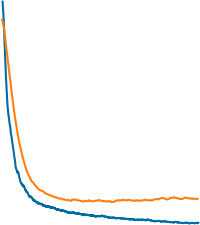
\includegraphics[interpolate=true,width=1.940000in,height=1.660000in]{sample-1000-img1.png}}%
\end{pgfscope}%
\begin{pgfscope}%
\pgfsetrectcap%
\pgfsetmiterjoin%
\pgfsetlinewidth{1.254687pt}%
\definecolor{currentstroke}{rgb}{0.150000,0.150000,0.150000}%
\pgfsetstrokecolor{currentstroke}%
\pgfsetdash{}{0pt}%
\pgfpathmoveto{\pgfqpoint{3.401003in}{0.558892in}}%
\pgfpathlineto{\pgfqpoint{3.401003in}{2.375154in}}%
\pgfusepath{stroke}%
\end{pgfscope}%
\begin{pgfscope}%
\pgfsetrectcap%
\pgfsetmiterjoin%
\pgfsetlinewidth{1.254687pt}%
\definecolor{currentstroke}{rgb}{0.150000,0.150000,0.150000}%
\pgfsetstrokecolor{currentstroke}%
\pgfsetdash{}{0pt}%
\pgfpathmoveto{\pgfqpoint{5.495496in}{0.558892in}}%
\pgfpathlineto{\pgfqpoint{5.495496in}{2.375154in}}%
\pgfusepath{stroke}%
\end{pgfscope}%
\begin{pgfscope}%
\pgfsetrectcap%
\pgfsetmiterjoin%
\pgfsetlinewidth{1.254687pt}%
\definecolor{currentstroke}{rgb}{0.150000,0.150000,0.150000}%
\pgfsetstrokecolor{currentstroke}%
\pgfsetdash{}{0pt}%
\pgfpathmoveto{\pgfqpoint{3.401003in}{0.558892in}}%
\pgfpathlineto{\pgfqpoint{5.495496in}{0.558892in}}%
\pgfusepath{stroke}%
\end{pgfscope}%
\begin{pgfscope}%
\pgfsetrectcap%
\pgfsetmiterjoin%
\pgfsetlinewidth{1.254687pt}%
\definecolor{currentstroke}{rgb}{0.150000,0.150000,0.150000}%
\pgfsetstrokecolor{currentstroke}%
\pgfsetdash{}{0pt}%
\pgfpathmoveto{\pgfqpoint{3.401003in}{2.375154in}}%
\pgfpathlineto{\pgfqpoint{5.495496in}{2.375154in}}%
\pgfusepath{stroke}%
\end{pgfscope}%
\begin{pgfscope}%
\pgfsetroundcap%
\pgfsetroundjoin%
\pgfsetlinewidth{1.505625pt}%
\definecolor{currentstroke}{rgb}{0.400000,0.760784,0.647059}%
\pgfsetstrokecolor{currentstroke}%
\pgfsetdash{}{0pt}%
\pgfpathmoveto{\pgfqpoint{3.501003in}{0.883979in}}%
\pgfpathlineto{\pgfqpoint{3.612115in}{0.883979in}}%
\pgfpathlineto{\pgfqpoint{3.723226in}{0.883979in}}%
\pgfusepath{stroke}%
\end{pgfscope}%
\begin{pgfscope}%
\definecolor{textcolor}{rgb}{0.150000,0.150000,0.150000}%
\pgfsetstrokecolor{textcolor}%
\pgfsetfillcolor{textcolor}%
\pgftext[x=3.812115in,y=0.845090in,left,base]{\color{textcolor}\rmfamily\fontsize{8.000000}{9.600000}\selectfont MAP train}%
\end{pgfscope}%
\begin{pgfscope}%
\pgfsetroundcap%
\pgfsetroundjoin%
\pgfsetlinewidth{1.505625pt}%
\definecolor{currentstroke}{rgb}{0.988235,0.552941,0.384314}%
\pgfsetstrokecolor{currentstroke}%
\pgfsetdash{}{0pt}%
\pgfpathmoveto{\pgfqpoint{3.501003in}{0.720893in}}%
\pgfpathlineto{\pgfqpoint{3.612115in}{0.720893in}}%
\pgfpathlineto{\pgfqpoint{3.723226in}{0.720893in}}%
\pgfusepath{stroke}%
\end{pgfscope}%
\begin{pgfscope}%
\definecolor{textcolor}{rgb}{0.150000,0.150000,0.150000}%
\pgfsetstrokecolor{textcolor}%
\pgfsetfillcolor{textcolor}%
\pgftext[x=3.812115in,y=0.682004in,left,base]{\color{textcolor}\rmfamily\fontsize{8.000000}{9.600000}\selectfont MAP test}%
\end{pgfscope}%
\begin{pgfscope}%
\definecolor{textcolor}{rgb}{0.150000,0.150000,0.150000}%
\pgfsetstrokecolor{textcolor}%
\pgfsetfillcolor{textcolor}%
\pgftext[x=2.822748in,y=2.766293in,,top]{\color{textcolor}\rmfamily\fontsize{12.000000}{14.400000}\selectfont 1000 training samples}%
\end{pgfscope}%
\end{pgfpicture}%
\makeatother%
\endgroup%

    \(5000\) samples
    %% Creator: Matplotlib, PGF backend
%%
%% To include the figure in your LaTeX document, write
%%   \input{<filename>.pgf}
%%
%% Make sure the required packages are loaded in your preamble
%%   \usepackage{pgf}
%%
%% Also ensure that all the required font packages are loaded; for instance,
%% the lmodern package is sometimes necessary when using math font.
%%   \usepackage{lmodern}
%%
%% Figures using additional raster images can only be included by \input if
%% they are in the same directory as the main LaTeX file. For loading figures
%% from other directories you can use the `import` package
%%   \usepackage{import}
%%
%% and then include the figures with
%%   \import{<path to file>}{<filename>.pgf}
%%
%% Matplotlib used the following preamble
%%   \usepackage{fontspec}
%%   \setmainfont{DejaVuSerif.ttf}[Path=\detokenize{/home/oslund/Thesis/repo/venv/lib/python3.8/site-packages/matplotlib/mpl-data/fonts/ttf/}]
%%   \setsansfont{DejaVuSans.ttf}[Path=\detokenize{/home/oslund/Thesis/repo/venv/lib/python3.8/site-packages/matplotlib/mpl-data/fonts/ttf/}]
%%   \setmonofont{DejaVuSansMono.ttf}[Path=\detokenize{/home/oslund/Thesis/repo/venv/lib/python3.8/site-packages/matplotlib/mpl-data/fonts/ttf/}]
%%
\begingroup%
\makeatletter%
\begin{pgfpicture}%
\pgfpathrectangle{\pgfpointorigin}{\pgfqpoint{5.559542in}{1.896475in}}%
\pgfusepath{use as bounding box, clip}%
\begin{pgfscope}%
\pgfsetbuttcap%
\pgfsetmiterjoin%
\definecolor{currentfill}{rgb}{1.000000,1.000000,1.000000}%
\pgfsetfillcolor{currentfill}%
\pgfsetlinewidth{0.000000pt}%
\definecolor{currentstroke}{rgb}{1.000000,1.000000,1.000000}%
\pgfsetstrokecolor{currentstroke}%
\pgfsetstrokeopacity{0.000000}%
\pgfsetdash{}{0pt}%
\pgfpathmoveto{\pgfqpoint{0.000000in}{0.000000in}}%
\pgfpathlineto{\pgfqpoint{5.559542in}{0.000000in}}%
\pgfpathlineto{\pgfqpoint{5.559542in}{1.896475in}}%
\pgfpathlineto{\pgfqpoint{0.000000in}{1.896475in}}%
\pgfpathlineto{\pgfqpoint{0.000000in}{0.000000in}}%
\pgfpathclose%
\pgfusepath{fill}%
\end{pgfscope}%
\begin{pgfscope}%
\pgfsetbuttcap%
\pgfsetmiterjoin%
\definecolor{currentfill}{rgb}{1.000000,1.000000,1.000000}%
\pgfsetfillcolor{currentfill}%
\pgfsetlinewidth{0.000000pt}%
\definecolor{currentstroke}{rgb}{0.000000,0.000000,0.000000}%
\pgfsetstrokecolor{currentstroke}%
\pgfsetstrokeopacity{0.000000}%
\pgfsetdash{}{0pt}%
\pgfpathmoveto{\pgfqpoint{0.600965in}{0.529443in}}%
\pgfpathlineto{\pgfqpoint{2.724862in}{0.529443in}}%
\pgfpathlineto{\pgfqpoint{2.724862in}{1.796475in}}%
\pgfpathlineto{\pgfqpoint{0.600965in}{1.796475in}}%
\pgfpathlineto{\pgfqpoint{0.600965in}{0.529443in}}%
\pgfpathclose%
\pgfusepath{fill}%
\end{pgfscope}%
\begin{pgfscope}%
\pgfsetbuttcap%
\pgfsetroundjoin%
\definecolor{currentfill}{rgb}{0.150000,0.150000,0.150000}%
\pgfsetfillcolor{currentfill}%
\pgfsetlinewidth{1.254687pt}%
\definecolor{currentstroke}{rgb}{0.150000,0.150000,0.150000}%
\pgfsetstrokecolor{currentstroke}%
\pgfsetdash{}{0pt}%
\pgfsys@defobject{currentmarker}{\pgfqpoint{0.000000in}{-0.083333in}}{\pgfqpoint{0.000000in}{0.000000in}}{%
\pgfpathmoveto{\pgfqpoint{0.000000in}{0.000000in}}%
\pgfpathlineto{\pgfqpoint{0.000000in}{-0.083333in}}%
\pgfusepath{stroke,fill}%
}%
\begin{pgfscope}%
\pgfsys@transformshift{0.658075in}{0.529443in}%
\pgfsys@useobject{currentmarker}{}%
\end{pgfscope}%
\end{pgfscope}%
\begin{pgfscope}%
\definecolor{textcolor}{rgb}{0.150000,0.150000,0.150000}%
\pgfsetstrokecolor{textcolor}%
\pgfsetfillcolor{textcolor}%
\pgftext[x=0.658075in,y=0.397499in,,top]{\color{textcolor}\rmfamily\fontsize{8.000000}{9.600000}\selectfont \(\displaystyle {0.0}\)}%
\end{pgfscope}%
\begin{pgfscope}%
\pgfsetbuttcap%
\pgfsetroundjoin%
\definecolor{currentfill}{rgb}{0.150000,0.150000,0.150000}%
\pgfsetfillcolor{currentfill}%
\pgfsetlinewidth{1.254687pt}%
\definecolor{currentstroke}{rgb}{0.150000,0.150000,0.150000}%
\pgfsetstrokecolor{currentstroke}%
\pgfsetdash{}{0pt}%
\pgfsys@defobject{currentmarker}{\pgfqpoint{0.000000in}{-0.083333in}}{\pgfqpoint{0.000000in}{0.000000in}}{%
\pgfpathmoveto{\pgfqpoint{0.000000in}{0.000000in}}%
\pgfpathlineto{\pgfqpoint{0.000000in}{-0.083333in}}%
\pgfusepath{stroke,fill}%
}%
\begin{pgfscope}%
\pgfsys@transformshift{1.052383in}{0.529443in}%
\pgfsys@useobject{currentmarker}{}%
\end{pgfscope}%
\end{pgfscope}%
\begin{pgfscope}%
\definecolor{textcolor}{rgb}{0.150000,0.150000,0.150000}%
\pgfsetstrokecolor{textcolor}%
\pgfsetfillcolor{textcolor}%
\pgftext[x=1.052383in,y=0.397499in,,top]{\color{textcolor}\rmfamily\fontsize{8.000000}{9.600000}\selectfont \(\displaystyle {0.5}\)}%
\end{pgfscope}%
\begin{pgfscope}%
\pgfsetbuttcap%
\pgfsetroundjoin%
\definecolor{currentfill}{rgb}{0.150000,0.150000,0.150000}%
\pgfsetfillcolor{currentfill}%
\pgfsetlinewidth{1.254687pt}%
\definecolor{currentstroke}{rgb}{0.150000,0.150000,0.150000}%
\pgfsetstrokecolor{currentstroke}%
\pgfsetdash{}{0pt}%
\pgfsys@defobject{currentmarker}{\pgfqpoint{0.000000in}{-0.083333in}}{\pgfqpoint{0.000000in}{0.000000in}}{%
\pgfpathmoveto{\pgfqpoint{0.000000in}{0.000000in}}%
\pgfpathlineto{\pgfqpoint{0.000000in}{-0.083333in}}%
\pgfusepath{stroke,fill}%
}%
\begin{pgfscope}%
\pgfsys@transformshift{1.446691in}{0.529443in}%
\pgfsys@useobject{currentmarker}{}%
\end{pgfscope}%
\end{pgfscope}%
\begin{pgfscope}%
\definecolor{textcolor}{rgb}{0.150000,0.150000,0.150000}%
\pgfsetstrokecolor{textcolor}%
\pgfsetfillcolor{textcolor}%
\pgftext[x=1.446691in,y=0.397499in,,top]{\color{textcolor}\rmfamily\fontsize{8.000000}{9.600000}\selectfont \(\displaystyle {1.0}\)}%
\end{pgfscope}%
\begin{pgfscope}%
\pgfsetbuttcap%
\pgfsetroundjoin%
\definecolor{currentfill}{rgb}{0.150000,0.150000,0.150000}%
\pgfsetfillcolor{currentfill}%
\pgfsetlinewidth{1.254687pt}%
\definecolor{currentstroke}{rgb}{0.150000,0.150000,0.150000}%
\pgfsetstrokecolor{currentstroke}%
\pgfsetdash{}{0pt}%
\pgfsys@defobject{currentmarker}{\pgfqpoint{0.000000in}{-0.083333in}}{\pgfqpoint{0.000000in}{0.000000in}}{%
\pgfpathmoveto{\pgfqpoint{0.000000in}{0.000000in}}%
\pgfpathlineto{\pgfqpoint{0.000000in}{-0.083333in}}%
\pgfusepath{stroke,fill}%
}%
\begin{pgfscope}%
\pgfsys@transformshift{1.840999in}{0.529443in}%
\pgfsys@useobject{currentmarker}{}%
\end{pgfscope}%
\end{pgfscope}%
\begin{pgfscope}%
\definecolor{textcolor}{rgb}{0.150000,0.150000,0.150000}%
\pgfsetstrokecolor{textcolor}%
\pgfsetfillcolor{textcolor}%
\pgftext[x=1.840999in,y=0.397499in,,top]{\color{textcolor}\rmfamily\fontsize{8.000000}{9.600000}\selectfont \(\displaystyle {1.5}\)}%
\end{pgfscope}%
\begin{pgfscope}%
\pgfsetbuttcap%
\pgfsetroundjoin%
\definecolor{currentfill}{rgb}{0.150000,0.150000,0.150000}%
\pgfsetfillcolor{currentfill}%
\pgfsetlinewidth{1.254687pt}%
\definecolor{currentstroke}{rgb}{0.150000,0.150000,0.150000}%
\pgfsetstrokecolor{currentstroke}%
\pgfsetdash{}{0pt}%
\pgfsys@defobject{currentmarker}{\pgfqpoint{0.000000in}{-0.083333in}}{\pgfqpoint{0.000000in}{0.000000in}}{%
\pgfpathmoveto{\pgfqpoint{0.000000in}{0.000000in}}%
\pgfpathlineto{\pgfqpoint{0.000000in}{-0.083333in}}%
\pgfusepath{stroke,fill}%
}%
\begin{pgfscope}%
\pgfsys@transformshift{2.235306in}{0.529443in}%
\pgfsys@useobject{currentmarker}{}%
\end{pgfscope}%
\end{pgfscope}%
\begin{pgfscope}%
\definecolor{textcolor}{rgb}{0.150000,0.150000,0.150000}%
\pgfsetstrokecolor{textcolor}%
\pgfsetfillcolor{textcolor}%
\pgftext[x=2.235306in,y=0.397499in,,top]{\color{textcolor}\rmfamily\fontsize{8.000000}{9.600000}\selectfont \(\displaystyle {2.0}\)}%
\end{pgfscope}%
\begin{pgfscope}%
\pgfsetbuttcap%
\pgfsetroundjoin%
\definecolor{currentfill}{rgb}{0.150000,0.150000,0.150000}%
\pgfsetfillcolor{currentfill}%
\pgfsetlinewidth{1.254687pt}%
\definecolor{currentstroke}{rgb}{0.150000,0.150000,0.150000}%
\pgfsetstrokecolor{currentstroke}%
\pgfsetdash{}{0pt}%
\pgfsys@defobject{currentmarker}{\pgfqpoint{0.000000in}{-0.083333in}}{\pgfqpoint{0.000000in}{0.000000in}}{%
\pgfpathmoveto{\pgfqpoint{0.000000in}{0.000000in}}%
\pgfpathlineto{\pgfqpoint{0.000000in}{-0.083333in}}%
\pgfusepath{stroke,fill}%
}%
\begin{pgfscope}%
\pgfsys@transformshift{2.629614in}{0.529443in}%
\pgfsys@useobject{currentmarker}{}%
\end{pgfscope}%
\end{pgfscope}%
\begin{pgfscope}%
\definecolor{textcolor}{rgb}{0.150000,0.150000,0.150000}%
\pgfsetstrokecolor{textcolor}%
\pgfsetfillcolor{textcolor}%
\pgftext[x=2.629614in,y=0.397499in,,top]{\color{textcolor}\rmfamily\fontsize{8.000000}{9.600000}\selectfont \(\displaystyle {2.5}\)}%
\end{pgfscope}%
\begin{pgfscope}%
\definecolor{textcolor}{rgb}{0.150000,0.150000,0.150000}%
\pgfsetstrokecolor{textcolor}%
\pgfsetfillcolor{textcolor}%
\pgftext[x=1.662914in,y=0.234413in,,top]{\color{textcolor}\rmfamily\fontsize{10.000000}{12.000000}\selectfont step}%
\end{pgfscope}%
\begin{pgfscope}%
\definecolor{textcolor}{rgb}{0.150000,0.150000,0.150000}%
\pgfsetstrokecolor{textcolor}%
\pgfsetfillcolor{textcolor}%
\pgftext[x=2.724862in,y=0.248302in,right,top]{\color{textcolor}\rmfamily\fontsize{8.000000}{9.600000}\selectfont \(\displaystyle \times{10^{7}}{}\)}%
\end{pgfscope}%
\begin{pgfscope}%
\pgfsetbuttcap%
\pgfsetroundjoin%
\definecolor{currentfill}{rgb}{0.150000,0.150000,0.150000}%
\pgfsetfillcolor{currentfill}%
\pgfsetlinewidth{1.254687pt}%
\definecolor{currentstroke}{rgb}{0.150000,0.150000,0.150000}%
\pgfsetstrokecolor{currentstroke}%
\pgfsetdash{}{0pt}%
\pgfsys@defobject{currentmarker}{\pgfqpoint{-0.083333in}{0.000000in}}{\pgfqpoint{-0.000000in}{0.000000in}}{%
\pgfpathmoveto{\pgfqpoint{-0.000000in}{0.000000in}}%
\pgfpathlineto{\pgfqpoint{-0.083333in}{0.000000in}}%
\pgfusepath{stroke,fill}%
}%
\begin{pgfscope}%
\pgfsys@transformshift{0.600965in}{0.801569in}%
\pgfsys@useobject{currentmarker}{}%
\end{pgfscope}%
\end{pgfscope}%
\begin{pgfscope}%
\definecolor{textcolor}{rgb}{0.150000,0.150000,0.150000}%
\pgfsetstrokecolor{textcolor}%
\pgfsetfillcolor{textcolor}%
\pgftext[x=0.291935in, y=0.759360in, left, base]{\color{textcolor}\rmfamily\fontsize{8.000000}{9.600000}\selectfont \(\displaystyle {200}\)}%
\end{pgfscope}%
\begin{pgfscope}%
\pgfsetbuttcap%
\pgfsetroundjoin%
\definecolor{currentfill}{rgb}{0.150000,0.150000,0.150000}%
\pgfsetfillcolor{currentfill}%
\pgfsetlinewidth{1.254687pt}%
\definecolor{currentstroke}{rgb}{0.150000,0.150000,0.150000}%
\pgfsetstrokecolor{currentstroke}%
\pgfsetdash{}{0pt}%
\pgfsys@defobject{currentmarker}{\pgfqpoint{-0.083333in}{0.000000in}}{\pgfqpoint{-0.000000in}{0.000000in}}{%
\pgfpathmoveto{\pgfqpoint{-0.000000in}{0.000000in}}%
\pgfpathlineto{\pgfqpoint{-0.083333in}{0.000000in}}%
\pgfusepath{stroke,fill}%
}%
\begin{pgfscope}%
\pgfsys@transformshift{0.600965in}{1.145415in}%
\pgfsys@useobject{currentmarker}{}%
\end{pgfscope}%
\end{pgfscope}%
\begin{pgfscope}%
\definecolor{textcolor}{rgb}{0.150000,0.150000,0.150000}%
\pgfsetstrokecolor{textcolor}%
\pgfsetfillcolor{textcolor}%
\pgftext[x=0.291935in, y=1.103205in, left, base]{\color{textcolor}\rmfamily\fontsize{8.000000}{9.600000}\selectfont \(\displaystyle {400}\)}%
\end{pgfscope}%
\begin{pgfscope}%
\pgfsetbuttcap%
\pgfsetroundjoin%
\definecolor{currentfill}{rgb}{0.150000,0.150000,0.150000}%
\pgfsetfillcolor{currentfill}%
\pgfsetlinewidth{1.254687pt}%
\definecolor{currentstroke}{rgb}{0.150000,0.150000,0.150000}%
\pgfsetstrokecolor{currentstroke}%
\pgfsetdash{}{0pt}%
\pgfsys@defobject{currentmarker}{\pgfqpoint{-0.083333in}{0.000000in}}{\pgfqpoint{-0.000000in}{0.000000in}}{%
\pgfpathmoveto{\pgfqpoint{-0.000000in}{0.000000in}}%
\pgfpathlineto{\pgfqpoint{-0.083333in}{0.000000in}}%
\pgfusepath{stroke,fill}%
}%
\begin{pgfscope}%
\pgfsys@transformshift{0.600965in}{1.489260in}%
\pgfsys@useobject{currentmarker}{}%
\end{pgfscope}%
\end{pgfscope}%
\begin{pgfscope}%
\definecolor{textcolor}{rgb}{0.150000,0.150000,0.150000}%
\pgfsetstrokecolor{textcolor}%
\pgfsetfillcolor{textcolor}%
\pgftext[x=0.291935in, y=1.447051in, left, base]{\color{textcolor}\rmfamily\fontsize{8.000000}{9.600000}\selectfont \(\displaystyle {600}\)}%
\end{pgfscope}%
\begin{pgfscope}%
\definecolor{textcolor}{rgb}{0.150000,0.150000,0.150000}%
\pgfsetstrokecolor{textcolor}%
\pgfsetfillcolor{textcolor}%
\pgftext[x=0.236379in,y=1.162959in,,bottom,rotate=90.000000]{\color{textcolor}\rmfamily\fontsize{10.000000}{12.000000}\selectfont length}%
\end{pgfscope}%
\begin{pgfscope}%
\pgfsys@transformshift{0.680556in}{0.577030in}%
\pgftext[left,bottom]{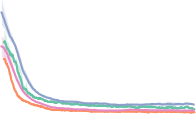
\includegraphics[interpolate=true,width=1.958333in,height=1.166667in]{sample-5000-img0.png}}%
\end{pgfscope}%
\begin{pgfscope}%
\pgfsetrectcap%
\pgfsetmiterjoin%
\pgfsetlinewidth{1.254687pt}%
\definecolor{currentstroke}{rgb}{0.150000,0.150000,0.150000}%
\pgfsetstrokecolor{currentstroke}%
\pgfsetdash{}{0pt}%
\pgfpathmoveto{\pgfqpoint{0.600965in}{0.529443in}}%
\pgfpathlineto{\pgfqpoint{0.600965in}{1.796475in}}%
\pgfusepath{stroke}%
\end{pgfscope}%
\begin{pgfscope}%
\pgfsetrectcap%
\pgfsetmiterjoin%
\pgfsetlinewidth{1.254687pt}%
\definecolor{currentstroke}{rgb}{0.150000,0.150000,0.150000}%
\pgfsetstrokecolor{currentstroke}%
\pgfsetdash{}{0pt}%
\pgfpathmoveto{\pgfqpoint{2.724862in}{0.529443in}}%
\pgfpathlineto{\pgfqpoint{2.724862in}{1.796475in}}%
\pgfusepath{stroke}%
\end{pgfscope}%
\begin{pgfscope}%
\pgfsetrectcap%
\pgfsetmiterjoin%
\pgfsetlinewidth{1.254687pt}%
\definecolor{currentstroke}{rgb}{0.150000,0.150000,0.150000}%
\pgfsetstrokecolor{currentstroke}%
\pgfsetdash{}{0pt}%
\pgfpathmoveto{\pgfqpoint{0.600965in}{0.529443in}}%
\pgfpathlineto{\pgfqpoint{2.724862in}{0.529443in}}%
\pgfusepath{stroke}%
\end{pgfscope}%
\begin{pgfscope}%
\pgfsetrectcap%
\pgfsetmiterjoin%
\pgfsetlinewidth{1.254687pt}%
\definecolor{currentstroke}{rgb}{0.150000,0.150000,0.150000}%
\pgfsetstrokecolor{currentstroke}%
\pgfsetdash{}{0pt}%
\pgfpathmoveto{\pgfqpoint{0.600965in}{1.796475in}}%
\pgfpathlineto{\pgfqpoint{2.724862in}{1.796475in}}%
\pgfusepath{stroke}%
\end{pgfscope}%
\begin{pgfscope}%
\pgfsetbuttcap%
\pgfsetmiterjoin%
\definecolor{currentfill}{rgb}{1.000000,1.000000,1.000000}%
\pgfsetfillcolor{currentfill}%
\pgfsetlinewidth{0.000000pt}%
\definecolor{currentstroke}{rgb}{0.000000,0.000000,0.000000}%
\pgfsetstrokecolor{currentstroke}%
\pgfsetstrokeopacity{0.000000}%
\pgfsetdash{}{0pt}%
\pgfpathmoveto{\pgfqpoint{3.335645in}{0.529443in}}%
\pgfpathlineto{\pgfqpoint{5.459542in}{0.529443in}}%
\pgfpathlineto{\pgfqpoint{5.459542in}{1.796475in}}%
\pgfpathlineto{\pgfqpoint{3.335645in}{1.796475in}}%
\pgfpathlineto{\pgfqpoint{3.335645in}{0.529443in}}%
\pgfpathclose%
\pgfusepath{fill}%
\end{pgfscope}%
\begin{pgfscope}%
\pgfsetbuttcap%
\pgfsetroundjoin%
\definecolor{currentfill}{rgb}{0.150000,0.150000,0.150000}%
\pgfsetfillcolor{currentfill}%
\pgfsetlinewidth{1.254687pt}%
\definecolor{currentstroke}{rgb}{0.150000,0.150000,0.150000}%
\pgfsetstrokecolor{currentstroke}%
\pgfsetdash{}{0pt}%
\pgfsys@defobject{currentmarker}{\pgfqpoint{0.000000in}{-0.083333in}}{\pgfqpoint{0.000000in}{0.000000in}}{%
\pgfpathmoveto{\pgfqpoint{0.000000in}{0.000000in}}%
\pgfpathlineto{\pgfqpoint{0.000000in}{-0.083333in}}%
\pgfusepath{stroke,fill}%
}%
\begin{pgfscope}%
\pgfsys@transformshift{3.392755in}{0.529443in}%
\pgfsys@useobject{currentmarker}{}%
\end{pgfscope}%
\end{pgfscope}%
\begin{pgfscope}%
\definecolor{textcolor}{rgb}{0.150000,0.150000,0.150000}%
\pgfsetstrokecolor{textcolor}%
\pgfsetfillcolor{textcolor}%
\pgftext[x=3.392755in,y=0.397499in,,top]{\color{textcolor}\rmfamily\fontsize{8.000000}{9.600000}\selectfont \(\displaystyle {0.0}\)}%
\end{pgfscope}%
\begin{pgfscope}%
\pgfsetbuttcap%
\pgfsetroundjoin%
\definecolor{currentfill}{rgb}{0.150000,0.150000,0.150000}%
\pgfsetfillcolor{currentfill}%
\pgfsetlinewidth{1.254687pt}%
\definecolor{currentstroke}{rgb}{0.150000,0.150000,0.150000}%
\pgfsetstrokecolor{currentstroke}%
\pgfsetdash{}{0pt}%
\pgfsys@defobject{currentmarker}{\pgfqpoint{0.000000in}{-0.083333in}}{\pgfqpoint{0.000000in}{0.000000in}}{%
\pgfpathmoveto{\pgfqpoint{0.000000in}{0.000000in}}%
\pgfpathlineto{\pgfqpoint{0.000000in}{-0.083333in}}%
\pgfusepath{stroke,fill}%
}%
\begin{pgfscope}%
\pgfsys@transformshift{3.787063in}{0.529443in}%
\pgfsys@useobject{currentmarker}{}%
\end{pgfscope}%
\end{pgfscope}%
\begin{pgfscope}%
\definecolor{textcolor}{rgb}{0.150000,0.150000,0.150000}%
\pgfsetstrokecolor{textcolor}%
\pgfsetfillcolor{textcolor}%
\pgftext[x=3.787063in,y=0.397499in,,top]{\color{textcolor}\rmfamily\fontsize{8.000000}{9.600000}\selectfont \(\displaystyle {0.5}\)}%
\end{pgfscope}%
\begin{pgfscope}%
\pgfsetbuttcap%
\pgfsetroundjoin%
\definecolor{currentfill}{rgb}{0.150000,0.150000,0.150000}%
\pgfsetfillcolor{currentfill}%
\pgfsetlinewidth{1.254687pt}%
\definecolor{currentstroke}{rgb}{0.150000,0.150000,0.150000}%
\pgfsetstrokecolor{currentstroke}%
\pgfsetdash{}{0pt}%
\pgfsys@defobject{currentmarker}{\pgfqpoint{0.000000in}{-0.083333in}}{\pgfqpoint{0.000000in}{0.000000in}}{%
\pgfpathmoveto{\pgfqpoint{0.000000in}{0.000000in}}%
\pgfpathlineto{\pgfqpoint{0.000000in}{-0.083333in}}%
\pgfusepath{stroke,fill}%
}%
\begin{pgfscope}%
\pgfsys@transformshift{4.181370in}{0.529443in}%
\pgfsys@useobject{currentmarker}{}%
\end{pgfscope}%
\end{pgfscope}%
\begin{pgfscope}%
\definecolor{textcolor}{rgb}{0.150000,0.150000,0.150000}%
\pgfsetstrokecolor{textcolor}%
\pgfsetfillcolor{textcolor}%
\pgftext[x=4.181370in,y=0.397499in,,top]{\color{textcolor}\rmfamily\fontsize{8.000000}{9.600000}\selectfont \(\displaystyle {1.0}\)}%
\end{pgfscope}%
\begin{pgfscope}%
\pgfsetbuttcap%
\pgfsetroundjoin%
\definecolor{currentfill}{rgb}{0.150000,0.150000,0.150000}%
\pgfsetfillcolor{currentfill}%
\pgfsetlinewidth{1.254687pt}%
\definecolor{currentstroke}{rgb}{0.150000,0.150000,0.150000}%
\pgfsetstrokecolor{currentstroke}%
\pgfsetdash{}{0pt}%
\pgfsys@defobject{currentmarker}{\pgfqpoint{0.000000in}{-0.083333in}}{\pgfqpoint{0.000000in}{0.000000in}}{%
\pgfpathmoveto{\pgfqpoint{0.000000in}{0.000000in}}%
\pgfpathlineto{\pgfqpoint{0.000000in}{-0.083333in}}%
\pgfusepath{stroke,fill}%
}%
\begin{pgfscope}%
\pgfsys@transformshift{4.575678in}{0.529443in}%
\pgfsys@useobject{currentmarker}{}%
\end{pgfscope}%
\end{pgfscope}%
\begin{pgfscope}%
\definecolor{textcolor}{rgb}{0.150000,0.150000,0.150000}%
\pgfsetstrokecolor{textcolor}%
\pgfsetfillcolor{textcolor}%
\pgftext[x=4.575678in,y=0.397499in,,top]{\color{textcolor}\rmfamily\fontsize{8.000000}{9.600000}\selectfont \(\displaystyle {1.5}\)}%
\end{pgfscope}%
\begin{pgfscope}%
\pgfsetbuttcap%
\pgfsetroundjoin%
\definecolor{currentfill}{rgb}{0.150000,0.150000,0.150000}%
\pgfsetfillcolor{currentfill}%
\pgfsetlinewidth{1.254687pt}%
\definecolor{currentstroke}{rgb}{0.150000,0.150000,0.150000}%
\pgfsetstrokecolor{currentstroke}%
\pgfsetdash{}{0pt}%
\pgfsys@defobject{currentmarker}{\pgfqpoint{0.000000in}{-0.083333in}}{\pgfqpoint{0.000000in}{0.000000in}}{%
\pgfpathmoveto{\pgfqpoint{0.000000in}{0.000000in}}%
\pgfpathlineto{\pgfqpoint{0.000000in}{-0.083333in}}%
\pgfusepath{stroke,fill}%
}%
\begin{pgfscope}%
\pgfsys@transformshift{4.969986in}{0.529443in}%
\pgfsys@useobject{currentmarker}{}%
\end{pgfscope}%
\end{pgfscope}%
\begin{pgfscope}%
\definecolor{textcolor}{rgb}{0.150000,0.150000,0.150000}%
\pgfsetstrokecolor{textcolor}%
\pgfsetfillcolor{textcolor}%
\pgftext[x=4.969986in,y=0.397499in,,top]{\color{textcolor}\rmfamily\fontsize{8.000000}{9.600000}\selectfont \(\displaystyle {2.0}\)}%
\end{pgfscope}%
\begin{pgfscope}%
\pgfsetbuttcap%
\pgfsetroundjoin%
\definecolor{currentfill}{rgb}{0.150000,0.150000,0.150000}%
\pgfsetfillcolor{currentfill}%
\pgfsetlinewidth{1.254687pt}%
\definecolor{currentstroke}{rgb}{0.150000,0.150000,0.150000}%
\pgfsetstrokecolor{currentstroke}%
\pgfsetdash{}{0pt}%
\pgfsys@defobject{currentmarker}{\pgfqpoint{0.000000in}{-0.083333in}}{\pgfqpoint{0.000000in}{0.000000in}}{%
\pgfpathmoveto{\pgfqpoint{0.000000in}{0.000000in}}%
\pgfpathlineto{\pgfqpoint{0.000000in}{-0.083333in}}%
\pgfusepath{stroke,fill}%
}%
\begin{pgfscope}%
\pgfsys@transformshift{5.364294in}{0.529443in}%
\pgfsys@useobject{currentmarker}{}%
\end{pgfscope}%
\end{pgfscope}%
\begin{pgfscope}%
\definecolor{textcolor}{rgb}{0.150000,0.150000,0.150000}%
\pgfsetstrokecolor{textcolor}%
\pgfsetfillcolor{textcolor}%
\pgftext[x=5.364294in,y=0.397499in,,top]{\color{textcolor}\rmfamily\fontsize{8.000000}{9.600000}\selectfont \(\displaystyle {2.5}\)}%
\end{pgfscope}%
\begin{pgfscope}%
\definecolor{textcolor}{rgb}{0.150000,0.150000,0.150000}%
\pgfsetstrokecolor{textcolor}%
\pgfsetfillcolor{textcolor}%
\pgftext[x=4.397593in,y=0.234413in,,top]{\color{textcolor}\rmfamily\fontsize{10.000000}{12.000000}\selectfont step}%
\end{pgfscope}%
\begin{pgfscope}%
\definecolor{textcolor}{rgb}{0.150000,0.150000,0.150000}%
\pgfsetstrokecolor{textcolor}%
\pgfsetfillcolor{textcolor}%
\pgftext[x=5.459542in,y=0.248302in,right,top]{\color{textcolor}\rmfamily\fontsize{8.000000}{9.600000}\selectfont \(\displaystyle \times{10^{7}}{}\)}%
\end{pgfscope}%
\begin{pgfscope}%
\pgfsetbuttcap%
\pgfsetroundjoin%
\definecolor{currentfill}{rgb}{0.150000,0.150000,0.150000}%
\pgfsetfillcolor{currentfill}%
\pgfsetlinewidth{1.254687pt}%
\definecolor{currentstroke}{rgb}{0.150000,0.150000,0.150000}%
\pgfsetstrokecolor{currentstroke}%
\pgfsetdash{}{0pt}%
\pgfsys@defobject{currentmarker}{\pgfqpoint{-0.083333in}{0.000000in}}{\pgfqpoint{-0.000000in}{0.000000in}}{%
\pgfpathmoveto{\pgfqpoint{-0.000000in}{0.000000in}}%
\pgfpathlineto{\pgfqpoint{-0.083333in}{0.000000in}}%
\pgfusepath{stroke,fill}%
}%
\begin{pgfscope}%
\pgfsys@transformshift{3.335645in}{0.868179in}%
\pgfsys@useobject{currentmarker}{}%
\end{pgfscope}%
\end{pgfscope}%
\begin{pgfscope}%
\definecolor{textcolor}{rgb}{0.150000,0.150000,0.150000}%
\pgfsetstrokecolor{textcolor}%
\pgfsetfillcolor{textcolor}%
\pgftext[x=3.052849in, y=0.825970in, left, base]{\color{textcolor}\rmfamily\fontsize{8.000000}{9.600000}\selectfont \(\displaystyle {0.6}\)}%
\end{pgfscope}%
\begin{pgfscope}%
\pgfsetbuttcap%
\pgfsetroundjoin%
\definecolor{currentfill}{rgb}{0.150000,0.150000,0.150000}%
\pgfsetfillcolor{currentfill}%
\pgfsetlinewidth{1.254687pt}%
\definecolor{currentstroke}{rgb}{0.150000,0.150000,0.150000}%
\pgfsetstrokecolor{currentstroke}%
\pgfsetdash{}{0pt}%
\pgfsys@defobject{currentmarker}{\pgfqpoint{-0.083333in}{0.000000in}}{\pgfqpoint{-0.000000in}{0.000000in}}{%
\pgfpathmoveto{\pgfqpoint{-0.000000in}{0.000000in}}%
\pgfpathlineto{\pgfqpoint{-0.083333in}{0.000000in}}%
\pgfusepath{stroke,fill}%
}%
\begin{pgfscope}%
\pgfsys@transformshift{3.335645in}{1.302101in}%
\pgfsys@useobject{currentmarker}{}%
\end{pgfscope}%
\end{pgfscope}%
\begin{pgfscope}%
\definecolor{textcolor}{rgb}{0.150000,0.150000,0.150000}%
\pgfsetstrokecolor{textcolor}%
\pgfsetfillcolor{textcolor}%
\pgftext[x=3.052849in, y=1.259892in, left, base]{\color{textcolor}\rmfamily\fontsize{8.000000}{9.600000}\selectfont \(\displaystyle {0.8}\)}%
\end{pgfscope}%
\begin{pgfscope}%
\pgfsetbuttcap%
\pgfsetroundjoin%
\definecolor{currentfill}{rgb}{0.150000,0.150000,0.150000}%
\pgfsetfillcolor{currentfill}%
\pgfsetlinewidth{1.254687pt}%
\definecolor{currentstroke}{rgb}{0.150000,0.150000,0.150000}%
\pgfsetstrokecolor{currentstroke}%
\pgfsetdash{}{0pt}%
\pgfsys@defobject{currentmarker}{\pgfqpoint{-0.083333in}{0.000000in}}{\pgfqpoint{-0.000000in}{0.000000in}}{%
\pgfpathmoveto{\pgfqpoint{-0.000000in}{0.000000in}}%
\pgfpathlineto{\pgfqpoint{-0.083333in}{0.000000in}}%
\pgfusepath{stroke,fill}%
}%
\begin{pgfscope}%
\pgfsys@transformshift{3.335645in}{1.736023in}%
\pgfsys@useobject{currentmarker}{}%
\end{pgfscope}%
\end{pgfscope}%
\begin{pgfscope}%
\definecolor{textcolor}{rgb}{0.150000,0.150000,0.150000}%
\pgfsetstrokecolor{textcolor}%
\pgfsetfillcolor{textcolor}%
\pgftext[x=3.052849in, y=1.693814in, left, base]{\color{textcolor}\rmfamily\fontsize{8.000000}{9.600000}\selectfont \(\displaystyle {1.0}\)}%
\end{pgfscope}%
\begin{pgfscope}%
\definecolor{textcolor}{rgb}{0.150000,0.150000,0.150000}%
\pgfsetstrokecolor{textcolor}%
\pgfsetfillcolor{textcolor}%
\pgftext[x=2.997294in,y=1.162959in,,bottom,rotate=90.000000]{\color{textcolor}\rmfamily\fontsize{10.000000}{12.000000}\selectfont success}%
\end{pgfscope}%
\begin{pgfscope}%
\pgfsys@transformshift{3.416667in}{0.577030in}%
\pgftext[left,bottom]{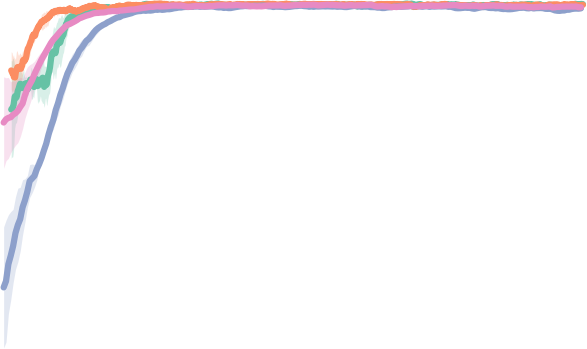
\includegraphics[interpolate=true,width=1.958333in,height=1.180556in]{sample-5000-img1.png}}%
\end{pgfscope}%
\begin{pgfscope}%
\pgfsetrectcap%
\pgfsetmiterjoin%
\pgfsetlinewidth{1.254687pt}%
\definecolor{currentstroke}{rgb}{0.150000,0.150000,0.150000}%
\pgfsetstrokecolor{currentstroke}%
\pgfsetdash{}{0pt}%
\pgfpathmoveto{\pgfqpoint{3.335645in}{0.529443in}}%
\pgfpathlineto{\pgfqpoint{3.335645in}{1.796475in}}%
\pgfusepath{stroke}%
\end{pgfscope}%
\begin{pgfscope}%
\pgfsetrectcap%
\pgfsetmiterjoin%
\pgfsetlinewidth{1.254687pt}%
\definecolor{currentstroke}{rgb}{0.150000,0.150000,0.150000}%
\pgfsetstrokecolor{currentstroke}%
\pgfsetdash{}{0pt}%
\pgfpathmoveto{\pgfqpoint{5.459542in}{0.529443in}}%
\pgfpathlineto{\pgfqpoint{5.459542in}{1.796475in}}%
\pgfusepath{stroke}%
\end{pgfscope}%
\begin{pgfscope}%
\pgfsetrectcap%
\pgfsetmiterjoin%
\pgfsetlinewidth{1.254687pt}%
\definecolor{currentstroke}{rgb}{0.150000,0.150000,0.150000}%
\pgfsetstrokecolor{currentstroke}%
\pgfsetdash{}{0pt}%
\pgfpathmoveto{\pgfqpoint{3.335645in}{0.529443in}}%
\pgfpathlineto{\pgfqpoint{5.459542in}{0.529443in}}%
\pgfusepath{stroke}%
\end{pgfscope}%
\begin{pgfscope}%
\pgfsetrectcap%
\pgfsetmiterjoin%
\pgfsetlinewidth{1.254687pt}%
\definecolor{currentstroke}{rgb}{0.150000,0.150000,0.150000}%
\pgfsetstrokecolor{currentstroke}%
\pgfsetdash{}{0pt}%
\pgfpathmoveto{\pgfqpoint{3.335645in}{1.796475in}}%
\pgfpathlineto{\pgfqpoint{5.459542in}{1.796475in}}%
\pgfusepath{stroke}%
\end{pgfscope}%
\end{pgfpicture}%
\makeatother%
\endgroup%

    \(10000\) samples
    %% Creator: Matplotlib, PGF backend
%%
%% To include the figure in your LaTeX document, write
%%   \input{<filename>.pgf}
%%
%% Make sure the required packages are loaded in your preamble
%%   \usepackage{pgf}
%%
%% Also ensure that all the required font packages are loaded; for instance,
%% the lmodern package is sometimes necessary when using math font.
%%   \usepackage{lmodern}
%%
%% Figures using additional raster images can only be included by \input if
%% they are in the same directory as the main LaTeX file. For loading figures
%% from other directories you can use the `import` package
%%   \usepackage{import}
%%
%% and then include the figures with
%%   \import{<path to file>}{<filename>.pgf}
%%
%% Matplotlib used the following preamble
%%   \usepackage{fontspec}
%%   \setmainfont{DejaVuSerif.ttf}[Path=\detokenize{/home/oslund/.local/lib/python3.8/site-packages/matplotlib/mpl-data/fonts/ttf/}]
%%   \setsansfont{DejaVuSans.ttf}[Path=\detokenize{/home/oslund/.local/lib/python3.8/site-packages/matplotlib/mpl-data/fonts/ttf/}]
%%   \setmonofont{DejaVuSansMono.ttf}[Path=\detokenize{/home/oslund/.local/lib/python3.8/site-packages/matplotlib/mpl-data/fonts/ttf/}]
%%
\begingroup%
\makeatletter%
\begin{pgfpicture}%
\pgfpathrectangle{\pgfpointorigin}{\pgfqpoint{5.645496in}{2.258198in}}%
\pgfusepath{use as bounding box, clip}%
\begin{pgfscope}%
\pgfsetbuttcap%
\pgfsetmiterjoin%
\definecolor{currentfill}{rgb}{1.000000,1.000000,1.000000}%
\pgfsetfillcolor{currentfill}%
\pgfsetlinewidth{0.000000pt}%
\definecolor{currentstroke}{rgb}{1.000000,1.000000,1.000000}%
\pgfsetstrokecolor{currentstroke}%
\pgfsetdash{}{0pt}%
\pgfpathmoveto{\pgfqpoint{0.000000in}{0.000000in}}%
\pgfpathlineto{\pgfqpoint{5.645496in}{0.000000in}}%
\pgfpathlineto{\pgfqpoint{5.645496in}{2.258198in}}%
\pgfpathlineto{\pgfqpoint{0.000000in}{2.258198in}}%
\pgfpathlineto{\pgfqpoint{0.000000in}{0.000000in}}%
\pgfpathclose%
\pgfusepath{fill}%
\end{pgfscope}%
\begin{pgfscope}%
\pgfsetbuttcap%
\pgfsetmiterjoin%
\definecolor{currentfill}{rgb}{1.000000,1.000000,1.000000}%
\pgfsetfillcolor{currentfill}%
\pgfsetlinewidth{0.000000pt}%
\definecolor{currentstroke}{rgb}{0.000000,0.000000,0.000000}%
\pgfsetstrokecolor{currentstroke}%
\pgfsetstrokeopacity{0.000000}%
\pgfsetdash{}{0pt}%
\pgfpathmoveto{\pgfqpoint{0.636920in}{0.558892in}}%
\pgfpathlineto{\pgfqpoint{2.760816in}{0.558892in}}%
\pgfpathlineto{\pgfqpoint{2.760816in}{1.772367in}}%
\pgfpathlineto{\pgfqpoint{0.636920in}{1.772367in}}%
\pgfpathlineto{\pgfqpoint{0.636920in}{0.558892in}}%
\pgfpathclose%
\pgfusepath{fill}%
\end{pgfscope}%
\begin{pgfscope}%
\pgfsetbuttcap%
\pgfsetroundjoin%
\definecolor{currentfill}{rgb}{0.150000,0.150000,0.150000}%
\pgfsetfillcolor{currentfill}%
\pgfsetlinewidth{1.254687pt}%
\definecolor{currentstroke}{rgb}{0.150000,0.150000,0.150000}%
\pgfsetstrokecolor{currentstroke}%
\pgfsetdash{}{0pt}%
\pgfsys@defobject{currentmarker}{\pgfqpoint{0.000000in}{-0.083333in}}{\pgfqpoint{0.000000in}{0.000000in}}{%
\pgfpathmoveto{\pgfqpoint{0.000000in}{0.000000in}}%
\pgfpathlineto{\pgfqpoint{0.000000in}{-0.083333in}}%
\pgfusepath{stroke,fill}%
}%
\begin{pgfscope}%
\pgfsys@transformshift{0.694030in}{0.558892in}%
\pgfsys@useobject{currentmarker}{}%
\end{pgfscope}%
\end{pgfscope}%
\begin{pgfscope}%
\definecolor{textcolor}{rgb}{0.150000,0.150000,0.150000}%
\pgfsetstrokecolor{textcolor}%
\pgfsetfillcolor{textcolor}%
\pgftext[x=0.694030in,y=0.426948in,,top]{\color{textcolor}\rmfamily\fontsize{8.000000}{9.600000}\selectfont \(\displaystyle {0.0}\)}%
\end{pgfscope}%
\begin{pgfscope}%
\pgfsetbuttcap%
\pgfsetroundjoin%
\definecolor{currentfill}{rgb}{0.150000,0.150000,0.150000}%
\pgfsetfillcolor{currentfill}%
\pgfsetlinewidth{1.254687pt}%
\definecolor{currentstroke}{rgb}{0.150000,0.150000,0.150000}%
\pgfsetstrokecolor{currentstroke}%
\pgfsetdash{}{0pt}%
\pgfsys@defobject{currentmarker}{\pgfqpoint{0.000000in}{-0.083333in}}{\pgfqpoint{0.000000in}{0.000000in}}{%
\pgfpathmoveto{\pgfqpoint{0.000000in}{0.000000in}}%
\pgfpathlineto{\pgfqpoint{0.000000in}{-0.083333in}}%
\pgfusepath{stroke,fill}%
}%
\begin{pgfscope}%
\pgfsys@transformshift{1.088338in}{0.558892in}%
\pgfsys@useobject{currentmarker}{}%
\end{pgfscope}%
\end{pgfscope}%
\begin{pgfscope}%
\definecolor{textcolor}{rgb}{0.150000,0.150000,0.150000}%
\pgfsetstrokecolor{textcolor}%
\pgfsetfillcolor{textcolor}%
\pgftext[x=1.088338in,y=0.426948in,,top]{\color{textcolor}\rmfamily\fontsize{8.000000}{9.600000}\selectfont \(\displaystyle {0.5}\)}%
\end{pgfscope}%
\begin{pgfscope}%
\pgfsetbuttcap%
\pgfsetroundjoin%
\definecolor{currentfill}{rgb}{0.150000,0.150000,0.150000}%
\pgfsetfillcolor{currentfill}%
\pgfsetlinewidth{1.254687pt}%
\definecolor{currentstroke}{rgb}{0.150000,0.150000,0.150000}%
\pgfsetstrokecolor{currentstroke}%
\pgfsetdash{}{0pt}%
\pgfsys@defobject{currentmarker}{\pgfqpoint{0.000000in}{-0.083333in}}{\pgfqpoint{0.000000in}{0.000000in}}{%
\pgfpathmoveto{\pgfqpoint{0.000000in}{0.000000in}}%
\pgfpathlineto{\pgfqpoint{0.000000in}{-0.083333in}}%
\pgfusepath{stroke,fill}%
}%
\begin{pgfscope}%
\pgfsys@transformshift{1.482645in}{0.558892in}%
\pgfsys@useobject{currentmarker}{}%
\end{pgfscope}%
\end{pgfscope}%
\begin{pgfscope}%
\definecolor{textcolor}{rgb}{0.150000,0.150000,0.150000}%
\pgfsetstrokecolor{textcolor}%
\pgfsetfillcolor{textcolor}%
\pgftext[x=1.482645in,y=0.426948in,,top]{\color{textcolor}\rmfamily\fontsize{8.000000}{9.600000}\selectfont \(\displaystyle {1.0}\)}%
\end{pgfscope}%
\begin{pgfscope}%
\pgfsetbuttcap%
\pgfsetroundjoin%
\definecolor{currentfill}{rgb}{0.150000,0.150000,0.150000}%
\pgfsetfillcolor{currentfill}%
\pgfsetlinewidth{1.254687pt}%
\definecolor{currentstroke}{rgb}{0.150000,0.150000,0.150000}%
\pgfsetstrokecolor{currentstroke}%
\pgfsetdash{}{0pt}%
\pgfsys@defobject{currentmarker}{\pgfqpoint{0.000000in}{-0.083333in}}{\pgfqpoint{0.000000in}{0.000000in}}{%
\pgfpathmoveto{\pgfqpoint{0.000000in}{0.000000in}}%
\pgfpathlineto{\pgfqpoint{0.000000in}{-0.083333in}}%
\pgfusepath{stroke,fill}%
}%
\begin{pgfscope}%
\pgfsys@transformshift{1.876953in}{0.558892in}%
\pgfsys@useobject{currentmarker}{}%
\end{pgfscope}%
\end{pgfscope}%
\begin{pgfscope}%
\definecolor{textcolor}{rgb}{0.150000,0.150000,0.150000}%
\pgfsetstrokecolor{textcolor}%
\pgfsetfillcolor{textcolor}%
\pgftext[x=1.876953in,y=0.426948in,,top]{\color{textcolor}\rmfamily\fontsize{8.000000}{9.600000}\selectfont \(\displaystyle {1.5}\)}%
\end{pgfscope}%
\begin{pgfscope}%
\pgfsetbuttcap%
\pgfsetroundjoin%
\definecolor{currentfill}{rgb}{0.150000,0.150000,0.150000}%
\pgfsetfillcolor{currentfill}%
\pgfsetlinewidth{1.254687pt}%
\definecolor{currentstroke}{rgb}{0.150000,0.150000,0.150000}%
\pgfsetstrokecolor{currentstroke}%
\pgfsetdash{}{0pt}%
\pgfsys@defobject{currentmarker}{\pgfqpoint{0.000000in}{-0.083333in}}{\pgfqpoint{0.000000in}{0.000000in}}{%
\pgfpathmoveto{\pgfqpoint{0.000000in}{0.000000in}}%
\pgfpathlineto{\pgfqpoint{0.000000in}{-0.083333in}}%
\pgfusepath{stroke,fill}%
}%
\begin{pgfscope}%
\pgfsys@transformshift{2.271261in}{0.558892in}%
\pgfsys@useobject{currentmarker}{}%
\end{pgfscope}%
\end{pgfscope}%
\begin{pgfscope}%
\definecolor{textcolor}{rgb}{0.150000,0.150000,0.150000}%
\pgfsetstrokecolor{textcolor}%
\pgfsetfillcolor{textcolor}%
\pgftext[x=2.271261in,y=0.426948in,,top]{\color{textcolor}\rmfamily\fontsize{8.000000}{9.600000}\selectfont \(\displaystyle {2.0}\)}%
\end{pgfscope}%
\begin{pgfscope}%
\pgfsetbuttcap%
\pgfsetroundjoin%
\definecolor{currentfill}{rgb}{0.150000,0.150000,0.150000}%
\pgfsetfillcolor{currentfill}%
\pgfsetlinewidth{1.254687pt}%
\definecolor{currentstroke}{rgb}{0.150000,0.150000,0.150000}%
\pgfsetstrokecolor{currentstroke}%
\pgfsetdash{}{0pt}%
\pgfsys@defobject{currentmarker}{\pgfqpoint{0.000000in}{-0.083333in}}{\pgfqpoint{0.000000in}{0.000000in}}{%
\pgfpathmoveto{\pgfqpoint{0.000000in}{0.000000in}}%
\pgfpathlineto{\pgfqpoint{0.000000in}{-0.083333in}}%
\pgfusepath{stroke,fill}%
}%
\begin{pgfscope}%
\pgfsys@transformshift{2.665569in}{0.558892in}%
\pgfsys@useobject{currentmarker}{}%
\end{pgfscope}%
\end{pgfscope}%
\begin{pgfscope}%
\definecolor{textcolor}{rgb}{0.150000,0.150000,0.150000}%
\pgfsetstrokecolor{textcolor}%
\pgfsetfillcolor{textcolor}%
\pgftext[x=2.665569in,y=0.426948in,,top]{\color{textcolor}\rmfamily\fontsize{8.000000}{9.600000}\selectfont \(\displaystyle {2.5}\)}%
\end{pgfscope}%
\begin{pgfscope}%
\definecolor{textcolor}{rgb}{0.150000,0.150000,0.150000}%
\pgfsetstrokecolor{textcolor}%
\pgfsetfillcolor{textcolor}%
\pgftext[x=1.698868in,y=0.263862in,,top]{\color{textcolor}\rmfamily\fontsize{10.000000}{12.000000}\selectfont step}%
\end{pgfscope}%
\begin{pgfscope}%
\definecolor{textcolor}{rgb}{0.150000,0.150000,0.150000}%
\pgfsetstrokecolor{textcolor}%
\pgfsetfillcolor{textcolor}%
\pgftext[x=2.760816in,y=0.277751in,right,top]{\color{textcolor}\rmfamily\fontsize{8.000000}{9.600000}\selectfont \(\displaystyle \times{10^{7}}{}\)}%
\end{pgfscope}%
\begin{pgfscope}%
\pgfsetbuttcap%
\pgfsetroundjoin%
\definecolor{currentfill}{rgb}{0.150000,0.150000,0.150000}%
\pgfsetfillcolor{currentfill}%
\pgfsetlinewidth{1.254687pt}%
\definecolor{currentstroke}{rgb}{0.150000,0.150000,0.150000}%
\pgfsetstrokecolor{currentstroke}%
\pgfsetdash{}{0pt}%
\pgfsys@defobject{currentmarker}{\pgfqpoint{-0.083333in}{0.000000in}}{\pgfqpoint{-0.000000in}{0.000000in}}{%
\pgfpathmoveto{\pgfqpoint{-0.000000in}{0.000000in}}%
\pgfpathlineto{\pgfqpoint{-0.083333in}{0.000000in}}%
\pgfusepath{stroke,fill}%
}%
\begin{pgfscope}%
\pgfsys@transformshift{0.636920in}{0.853928in}%
\pgfsys@useobject{currentmarker}{}%
\end{pgfscope}%
\end{pgfscope}%
\begin{pgfscope}%
\definecolor{textcolor}{rgb}{0.150000,0.150000,0.150000}%
\pgfsetstrokecolor{textcolor}%
\pgfsetfillcolor{textcolor}%
\pgftext[x=0.327890in, y=0.811718in, left, base]{\color{textcolor}\rmfamily\fontsize{8.000000}{9.600000}\selectfont \(\displaystyle {200}\)}%
\end{pgfscope}%
\begin{pgfscope}%
\pgfsetbuttcap%
\pgfsetroundjoin%
\definecolor{currentfill}{rgb}{0.150000,0.150000,0.150000}%
\pgfsetfillcolor{currentfill}%
\pgfsetlinewidth{1.254687pt}%
\definecolor{currentstroke}{rgb}{0.150000,0.150000,0.150000}%
\pgfsetstrokecolor{currentstroke}%
\pgfsetdash{}{0pt}%
\pgfsys@defobject{currentmarker}{\pgfqpoint{-0.083333in}{0.000000in}}{\pgfqpoint{-0.000000in}{0.000000in}}{%
\pgfpathmoveto{\pgfqpoint{-0.000000in}{0.000000in}}%
\pgfpathlineto{\pgfqpoint{-0.083333in}{0.000000in}}%
\pgfusepath{stroke,fill}%
}%
\begin{pgfscope}%
\pgfsys@transformshift{0.636920in}{1.221248in}%
\pgfsys@useobject{currentmarker}{}%
\end{pgfscope}%
\end{pgfscope}%
\begin{pgfscope}%
\definecolor{textcolor}{rgb}{0.150000,0.150000,0.150000}%
\pgfsetstrokecolor{textcolor}%
\pgfsetfillcolor{textcolor}%
\pgftext[x=0.327890in, y=1.179039in, left, base]{\color{textcolor}\rmfamily\fontsize{8.000000}{9.600000}\selectfont \(\displaystyle {400}\)}%
\end{pgfscope}%
\begin{pgfscope}%
\pgfsetbuttcap%
\pgfsetroundjoin%
\definecolor{currentfill}{rgb}{0.150000,0.150000,0.150000}%
\pgfsetfillcolor{currentfill}%
\pgfsetlinewidth{1.254687pt}%
\definecolor{currentstroke}{rgb}{0.150000,0.150000,0.150000}%
\pgfsetstrokecolor{currentstroke}%
\pgfsetdash{}{0pt}%
\pgfsys@defobject{currentmarker}{\pgfqpoint{-0.083333in}{0.000000in}}{\pgfqpoint{-0.000000in}{0.000000in}}{%
\pgfpathmoveto{\pgfqpoint{-0.000000in}{0.000000in}}%
\pgfpathlineto{\pgfqpoint{-0.083333in}{0.000000in}}%
\pgfusepath{stroke,fill}%
}%
\begin{pgfscope}%
\pgfsys@transformshift{0.636920in}{1.588568in}%
\pgfsys@useobject{currentmarker}{}%
\end{pgfscope}%
\end{pgfscope}%
\begin{pgfscope}%
\definecolor{textcolor}{rgb}{0.150000,0.150000,0.150000}%
\pgfsetstrokecolor{textcolor}%
\pgfsetfillcolor{textcolor}%
\pgftext[x=0.327890in, y=1.546359in, left, base]{\color{textcolor}\rmfamily\fontsize{8.000000}{9.600000}\selectfont \(\displaystyle {600}\)}%
\end{pgfscope}%
\begin{pgfscope}%
\definecolor{textcolor}{rgb}{0.150000,0.150000,0.150000}%
\pgfsetstrokecolor{textcolor}%
\pgfsetfillcolor{textcolor}%
\pgftext[x=0.272334in,y=1.165630in,,bottom,rotate=90.000000]{\color{textcolor}\rmfamily\fontsize{10.000000}{12.000000}\selectfont length}%
\end{pgfscope}%
\begin{pgfscope}%
\pgfsys@transformshift{0.720000in}{0.608198in}%
\pgftext[left,bottom]{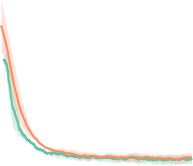
\includegraphics[interpolate=true,width=1.960000in,height=1.120000in]{sample-10000-img0.png}}%
\end{pgfscope}%
\begin{pgfscope}%
\pgfsetrectcap%
\pgfsetmiterjoin%
\pgfsetlinewidth{1.254687pt}%
\definecolor{currentstroke}{rgb}{0.150000,0.150000,0.150000}%
\pgfsetstrokecolor{currentstroke}%
\pgfsetdash{}{0pt}%
\pgfpathmoveto{\pgfqpoint{0.636920in}{0.558892in}}%
\pgfpathlineto{\pgfqpoint{0.636920in}{1.772367in}}%
\pgfusepath{stroke}%
\end{pgfscope}%
\begin{pgfscope}%
\pgfsetrectcap%
\pgfsetmiterjoin%
\pgfsetlinewidth{1.254687pt}%
\definecolor{currentstroke}{rgb}{0.150000,0.150000,0.150000}%
\pgfsetstrokecolor{currentstroke}%
\pgfsetdash{}{0pt}%
\pgfpathmoveto{\pgfqpoint{2.760816in}{0.558892in}}%
\pgfpathlineto{\pgfqpoint{2.760816in}{1.772367in}}%
\pgfusepath{stroke}%
\end{pgfscope}%
\begin{pgfscope}%
\pgfsetrectcap%
\pgfsetmiterjoin%
\pgfsetlinewidth{1.254687pt}%
\definecolor{currentstroke}{rgb}{0.150000,0.150000,0.150000}%
\pgfsetstrokecolor{currentstroke}%
\pgfsetdash{}{0pt}%
\pgfpathmoveto{\pgfqpoint{0.636920in}{0.558892in}}%
\pgfpathlineto{\pgfqpoint{2.760816in}{0.558892in}}%
\pgfusepath{stroke}%
\end{pgfscope}%
\begin{pgfscope}%
\pgfsetrectcap%
\pgfsetmiterjoin%
\pgfsetlinewidth{1.254687pt}%
\definecolor{currentstroke}{rgb}{0.150000,0.150000,0.150000}%
\pgfsetstrokecolor{currentstroke}%
\pgfsetdash{}{0pt}%
\pgfpathmoveto{\pgfqpoint{0.636920in}{1.772367in}}%
\pgfpathlineto{\pgfqpoint{2.760816in}{1.772367in}}%
\pgfusepath{stroke}%
\end{pgfscope}%
\begin{pgfscope}%
\pgfsetroundcap%
\pgfsetroundjoin%
\pgfsetlinewidth{1.505625pt}%
\definecolor{currentstroke}{rgb}{0.400000,0.760784,0.647059}%
\pgfsetstrokecolor{currentstroke}%
\pgfsetdash{}{0pt}%
\pgfpathmoveto{\pgfqpoint{1.800552in}{1.626838in}}%
\pgfpathlineto{\pgfqpoint{1.911663in}{1.626838in}}%
\pgfpathlineto{\pgfqpoint{2.022774in}{1.626838in}}%
\pgfusepath{stroke}%
\end{pgfscope}%
\begin{pgfscope}%
\definecolor{textcolor}{rgb}{0.150000,0.150000,0.150000}%
\pgfsetstrokecolor{textcolor}%
\pgfsetfillcolor{textcolor}%
\pgftext[x=2.111663in,y=1.587949in,left,base]{\color{textcolor}\rmfamily\fontsize{8.000000}{9.600000}\selectfont lstm train}%
\end{pgfscope}%
\begin{pgfscope}%
\pgfsetroundcap%
\pgfsetroundjoin%
\pgfsetlinewidth{1.505625pt}%
\definecolor{currentstroke}{rgb}{0.988235,0.552941,0.384314}%
\pgfsetstrokecolor{currentstroke}%
\pgfsetdash{}{0pt}%
\pgfpathmoveto{\pgfqpoint{1.800552in}{1.463752in}}%
\pgfpathlineto{\pgfqpoint{1.911663in}{1.463752in}}%
\pgfpathlineto{\pgfqpoint{2.022774in}{1.463752in}}%
\pgfusepath{stroke}%
\end{pgfscope}%
\begin{pgfscope}%
\definecolor{textcolor}{rgb}{0.150000,0.150000,0.150000}%
\pgfsetstrokecolor{textcolor}%
\pgfsetfillcolor{textcolor}%
\pgftext[x=2.111663in,y=1.424863in,left,base]{\color{textcolor}\rmfamily\fontsize{8.000000}{9.600000}\selectfont map train}%
\end{pgfscope}%
\begin{pgfscope}%
\pgfsetroundcap%
\pgfsetroundjoin%
\pgfsetlinewidth{1.505625pt}%
\definecolor{currentstroke}{rgb}{0.552941,0.627451,0.796078}%
\pgfsetstrokecolor{currentstroke}%
\pgfsetdash{}{0pt}%
\pgfpathmoveto{\pgfqpoint{1.800552in}{1.300666in}}%
\pgfpathlineto{\pgfqpoint{1.911663in}{1.300666in}}%
\pgfpathlineto{\pgfqpoint{2.022774in}{1.300666in}}%
\pgfusepath{stroke}%
\end{pgfscope}%
\begin{pgfscope}%
\definecolor{textcolor}{rgb}{0.150000,0.150000,0.150000}%
\pgfsetstrokecolor{textcolor}%
\pgfsetfillcolor{textcolor}%
\pgftext[x=2.111663in,y=1.261777in,left,base]{\color{textcolor}\rmfamily\fontsize{8.000000}{9.600000}\selectfont lstm test}%
\end{pgfscope}%
\begin{pgfscope}%
\pgfsetroundcap%
\pgfsetroundjoin%
\pgfsetlinewidth{1.505625pt}%
\definecolor{currentstroke}{rgb}{0.905882,0.541176,0.764706}%
\pgfsetstrokecolor{currentstroke}%
\pgfsetdash{}{0pt}%
\pgfpathmoveto{\pgfqpoint{1.800552in}{1.137580in}}%
\pgfpathlineto{\pgfqpoint{1.911663in}{1.137580in}}%
\pgfpathlineto{\pgfqpoint{2.022774in}{1.137580in}}%
\pgfusepath{stroke}%
\end{pgfscope}%
\begin{pgfscope}%
\definecolor{textcolor}{rgb}{0.150000,0.150000,0.150000}%
\pgfsetstrokecolor{textcolor}%
\pgfsetfillcolor{textcolor}%
\pgftext[x=2.111663in,y=1.098691in,left,base]{\color{textcolor}\rmfamily\fontsize{8.000000}{9.600000}\selectfont map test}%
\end{pgfscope}%
\begin{pgfscope}%
\pgfsetbuttcap%
\pgfsetmiterjoin%
\definecolor{currentfill}{rgb}{1.000000,1.000000,1.000000}%
\pgfsetfillcolor{currentfill}%
\pgfsetlinewidth{0.000000pt}%
\definecolor{currentstroke}{rgb}{0.000000,0.000000,0.000000}%
\pgfsetstrokecolor{currentstroke}%
\pgfsetstrokeopacity{0.000000}%
\pgfsetdash{}{0pt}%
\pgfpathmoveto{\pgfqpoint{3.371599in}{0.558892in}}%
\pgfpathlineto{\pgfqpoint{5.495496in}{0.558892in}}%
\pgfpathlineto{\pgfqpoint{5.495496in}{1.772367in}}%
\pgfpathlineto{\pgfqpoint{3.371599in}{1.772367in}}%
\pgfpathlineto{\pgfqpoint{3.371599in}{0.558892in}}%
\pgfpathclose%
\pgfusepath{fill}%
\end{pgfscope}%
\begin{pgfscope}%
\pgfsetbuttcap%
\pgfsetroundjoin%
\definecolor{currentfill}{rgb}{0.150000,0.150000,0.150000}%
\pgfsetfillcolor{currentfill}%
\pgfsetlinewidth{1.254687pt}%
\definecolor{currentstroke}{rgb}{0.150000,0.150000,0.150000}%
\pgfsetstrokecolor{currentstroke}%
\pgfsetdash{}{0pt}%
\pgfsys@defobject{currentmarker}{\pgfqpoint{0.000000in}{-0.083333in}}{\pgfqpoint{0.000000in}{0.000000in}}{%
\pgfpathmoveto{\pgfqpoint{0.000000in}{0.000000in}}%
\pgfpathlineto{\pgfqpoint{0.000000in}{-0.083333in}}%
\pgfusepath{stroke,fill}%
}%
\begin{pgfscope}%
\pgfsys@transformshift{3.428709in}{0.558892in}%
\pgfsys@useobject{currentmarker}{}%
\end{pgfscope}%
\end{pgfscope}%
\begin{pgfscope}%
\definecolor{textcolor}{rgb}{0.150000,0.150000,0.150000}%
\pgfsetstrokecolor{textcolor}%
\pgfsetfillcolor{textcolor}%
\pgftext[x=3.428709in,y=0.426948in,,top]{\color{textcolor}\rmfamily\fontsize{8.000000}{9.600000}\selectfont \(\displaystyle {0.0}\)}%
\end{pgfscope}%
\begin{pgfscope}%
\pgfsetbuttcap%
\pgfsetroundjoin%
\definecolor{currentfill}{rgb}{0.150000,0.150000,0.150000}%
\pgfsetfillcolor{currentfill}%
\pgfsetlinewidth{1.254687pt}%
\definecolor{currentstroke}{rgb}{0.150000,0.150000,0.150000}%
\pgfsetstrokecolor{currentstroke}%
\pgfsetdash{}{0pt}%
\pgfsys@defobject{currentmarker}{\pgfqpoint{0.000000in}{-0.083333in}}{\pgfqpoint{0.000000in}{0.000000in}}{%
\pgfpathmoveto{\pgfqpoint{0.000000in}{0.000000in}}%
\pgfpathlineto{\pgfqpoint{0.000000in}{-0.083333in}}%
\pgfusepath{stroke,fill}%
}%
\begin{pgfscope}%
\pgfsys@transformshift{3.823017in}{0.558892in}%
\pgfsys@useobject{currentmarker}{}%
\end{pgfscope}%
\end{pgfscope}%
\begin{pgfscope}%
\definecolor{textcolor}{rgb}{0.150000,0.150000,0.150000}%
\pgfsetstrokecolor{textcolor}%
\pgfsetfillcolor{textcolor}%
\pgftext[x=3.823017in,y=0.426948in,,top]{\color{textcolor}\rmfamily\fontsize{8.000000}{9.600000}\selectfont \(\displaystyle {0.5}\)}%
\end{pgfscope}%
\begin{pgfscope}%
\pgfsetbuttcap%
\pgfsetroundjoin%
\definecolor{currentfill}{rgb}{0.150000,0.150000,0.150000}%
\pgfsetfillcolor{currentfill}%
\pgfsetlinewidth{1.254687pt}%
\definecolor{currentstroke}{rgb}{0.150000,0.150000,0.150000}%
\pgfsetstrokecolor{currentstroke}%
\pgfsetdash{}{0pt}%
\pgfsys@defobject{currentmarker}{\pgfqpoint{0.000000in}{-0.083333in}}{\pgfqpoint{0.000000in}{0.000000in}}{%
\pgfpathmoveto{\pgfqpoint{0.000000in}{0.000000in}}%
\pgfpathlineto{\pgfqpoint{0.000000in}{-0.083333in}}%
\pgfusepath{stroke,fill}%
}%
\begin{pgfscope}%
\pgfsys@transformshift{4.217325in}{0.558892in}%
\pgfsys@useobject{currentmarker}{}%
\end{pgfscope}%
\end{pgfscope}%
\begin{pgfscope}%
\definecolor{textcolor}{rgb}{0.150000,0.150000,0.150000}%
\pgfsetstrokecolor{textcolor}%
\pgfsetfillcolor{textcolor}%
\pgftext[x=4.217325in,y=0.426948in,,top]{\color{textcolor}\rmfamily\fontsize{8.000000}{9.600000}\selectfont \(\displaystyle {1.0}\)}%
\end{pgfscope}%
\begin{pgfscope}%
\pgfsetbuttcap%
\pgfsetroundjoin%
\definecolor{currentfill}{rgb}{0.150000,0.150000,0.150000}%
\pgfsetfillcolor{currentfill}%
\pgfsetlinewidth{1.254687pt}%
\definecolor{currentstroke}{rgb}{0.150000,0.150000,0.150000}%
\pgfsetstrokecolor{currentstroke}%
\pgfsetdash{}{0pt}%
\pgfsys@defobject{currentmarker}{\pgfqpoint{0.000000in}{-0.083333in}}{\pgfqpoint{0.000000in}{0.000000in}}{%
\pgfpathmoveto{\pgfqpoint{0.000000in}{0.000000in}}%
\pgfpathlineto{\pgfqpoint{0.000000in}{-0.083333in}}%
\pgfusepath{stroke,fill}%
}%
\begin{pgfscope}%
\pgfsys@transformshift{4.611633in}{0.558892in}%
\pgfsys@useobject{currentmarker}{}%
\end{pgfscope}%
\end{pgfscope}%
\begin{pgfscope}%
\definecolor{textcolor}{rgb}{0.150000,0.150000,0.150000}%
\pgfsetstrokecolor{textcolor}%
\pgfsetfillcolor{textcolor}%
\pgftext[x=4.611633in,y=0.426948in,,top]{\color{textcolor}\rmfamily\fontsize{8.000000}{9.600000}\selectfont \(\displaystyle {1.5}\)}%
\end{pgfscope}%
\begin{pgfscope}%
\pgfsetbuttcap%
\pgfsetroundjoin%
\definecolor{currentfill}{rgb}{0.150000,0.150000,0.150000}%
\pgfsetfillcolor{currentfill}%
\pgfsetlinewidth{1.254687pt}%
\definecolor{currentstroke}{rgb}{0.150000,0.150000,0.150000}%
\pgfsetstrokecolor{currentstroke}%
\pgfsetdash{}{0pt}%
\pgfsys@defobject{currentmarker}{\pgfqpoint{0.000000in}{-0.083333in}}{\pgfqpoint{0.000000in}{0.000000in}}{%
\pgfpathmoveto{\pgfqpoint{0.000000in}{0.000000in}}%
\pgfpathlineto{\pgfqpoint{0.000000in}{-0.083333in}}%
\pgfusepath{stroke,fill}%
}%
\begin{pgfscope}%
\pgfsys@transformshift{5.005940in}{0.558892in}%
\pgfsys@useobject{currentmarker}{}%
\end{pgfscope}%
\end{pgfscope}%
\begin{pgfscope}%
\definecolor{textcolor}{rgb}{0.150000,0.150000,0.150000}%
\pgfsetstrokecolor{textcolor}%
\pgfsetfillcolor{textcolor}%
\pgftext[x=5.005940in,y=0.426948in,,top]{\color{textcolor}\rmfamily\fontsize{8.000000}{9.600000}\selectfont \(\displaystyle {2.0}\)}%
\end{pgfscope}%
\begin{pgfscope}%
\pgfsetbuttcap%
\pgfsetroundjoin%
\definecolor{currentfill}{rgb}{0.150000,0.150000,0.150000}%
\pgfsetfillcolor{currentfill}%
\pgfsetlinewidth{1.254687pt}%
\definecolor{currentstroke}{rgb}{0.150000,0.150000,0.150000}%
\pgfsetstrokecolor{currentstroke}%
\pgfsetdash{}{0pt}%
\pgfsys@defobject{currentmarker}{\pgfqpoint{0.000000in}{-0.083333in}}{\pgfqpoint{0.000000in}{0.000000in}}{%
\pgfpathmoveto{\pgfqpoint{0.000000in}{0.000000in}}%
\pgfpathlineto{\pgfqpoint{0.000000in}{-0.083333in}}%
\pgfusepath{stroke,fill}%
}%
\begin{pgfscope}%
\pgfsys@transformshift{5.400248in}{0.558892in}%
\pgfsys@useobject{currentmarker}{}%
\end{pgfscope}%
\end{pgfscope}%
\begin{pgfscope}%
\definecolor{textcolor}{rgb}{0.150000,0.150000,0.150000}%
\pgfsetstrokecolor{textcolor}%
\pgfsetfillcolor{textcolor}%
\pgftext[x=5.400248in,y=0.426948in,,top]{\color{textcolor}\rmfamily\fontsize{8.000000}{9.600000}\selectfont \(\displaystyle {2.5}\)}%
\end{pgfscope}%
\begin{pgfscope}%
\definecolor{textcolor}{rgb}{0.150000,0.150000,0.150000}%
\pgfsetstrokecolor{textcolor}%
\pgfsetfillcolor{textcolor}%
\pgftext[x=4.433548in,y=0.263862in,,top]{\color{textcolor}\rmfamily\fontsize{10.000000}{12.000000}\selectfont step}%
\end{pgfscope}%
\begin{pgfscope}%
\definecolor{textcolor}{rgb}{0.150000,0.150000,0.150000}%
\pgfsetstrokecolor{textcolor}%
\pgfsetfillcolor{textcolor}%
\pgftext[x=5.495496in,y=0.277751in,right,top]{\color{textcolor}\rmfamily\fontsize{8.000000}{9.600000}\selectfont \(\displaystyle \times{10^{7}}{}\)}%
\end{pgfscope}%
\begin{pgfscope}%
\pgfsetbuttcap%
\pgfsetroundjoin%
\definecolor{currentfill}{rgb}{0.150000,0.150000,0.150000}%
\pgfsetfillcolor{currentfill}%
\pgfsetlinewidth{1.254687pt}%
\definecolor{currentstroke}{rgb}{0.150000,0.150000,0.150000}%
\pgfsetstrokecolor{currentstroke}%
\pgfsetdash{}{0pt}%
\pgfsys@defobject{currentmarker}{\pgfqpoint{-0.083333in}{0.000000in}}{\pgfqpoint{-0.000000in}{0.000000in}}{%
\pgfpathmoveto{\pgfqpoint{-0.000000in}{0.000000in}}%
\pgfpathlineto{\pgfqpoint{-0.083333in}{0.000000in}}%
\pgfusepath{stroke,fill}%
}%
\begin{pgfscope}%
\pgfsys@transformshift{3.371599in}{0.697120in}%
\pgfsys@useobject{currentmarker}{}%
\end{pgfscope}%
\end{pgfscope}%
\begin{pgfscope}%
\definecolor{textcolor}{rgb}{0.150000,0.150000,0.150000}%
\pgfsetstrokecolor{textcolor}%
\pgfsetfillcolor{textcolor}%
\pgftext[x=3.088804in, y=0.654911in, left, base]{\color{textcolor}\rmfamily\fontsize{8.000000}{9.600000}\selectfont \(\displaystyle {0.6}\)}%
\end{pgfscope}%
\begin{pgfscope}%
\pgfsetbuttcap%
\pgfsetroundjoin%
\definecolor{currentfill}{rgb}{0.150000,0.150000,0.150000}%
\pgfsetfillcolor{currentfill}%
\pgfsetlinewidth{1.254687pt}%
\definecolor{currentstroke}{rgb}{0.150000,0.150000,0.150000}%
\pgfsetstrokecolor{currentstroke}%
\pgfsetdash{}{0pt}%
\pgfsys@defobject{currentmarker}{\pgfqpoint{-0.083333in}{0.000000in}}{\pgfqpoint{-0.000000in}{0.000000in}}{%
\pgfpathmoveto{\pgfqpoint{-0.000000in}{0.000000in}}%
\pgfpathlineto{\pgfqpoint{-0.083333in}{0.000000in}}%
\pgfusepath{stroke,fill}%
}%
\begin{pgfscope}%
\pgfsys@transformshift{3.371599in}{0.949960in}%
\pgfsys@useobject{currentmarker}{}%
\end{pgfscope}%
\end{pgfscope}%
\begin{pgfscope}%
\definecolor{textcolor}{rgb}{0.150000,0.150000,0.150000}%
\pgfsetstrokecolor{textcolor}%
\pgfsetfillcolor{textcolor}%
\pgftext[x=3.088804in, y=0.907751in, left, base]{\color{textcolor}\rmfamily\fontsize{8.000000}{9.600000}\selectfont \(\displaystyle {0.7}\)}%
\end{pgfscope}%
\begin{pgfscope}%
\pgfsetbuttcap%
\pgfsetroundjoin%
\definecolor{currentfill}{rgb}{0.150000,0.150000,0.150000}%
\pgfsetfillcolor{currentfill}%
\pgfsetlinewidth{1.254687pt}%
\definecolor{currentstroke}{rgb}{0.150000,0.150000,0.150000}%
\pgfsetstrokecolor{currentstroke}%
\pgfsetdash{}{0pt}%
\pgfsys@defobject{currentmarker}{\pgfqpoint{-0.083333in}{0.000000in}}{\pgfqpoint{-0.000000in}{0.000000in}}{%
\pgfpathmoveto{\pgfqpoint{-0.000000in}{0.000000in}}%
\pgfpathlineto{\pgfqpoint{-0.083333in}{0.000000in}}%
\pgfusepath{stroke,fill}%
}%
\begin{pgfscope}%
\pgfsys@transformshift{3.371599in}{1.202801in}%
\pgfsys@useobject{currentmarker}{}%
\end{pgfscope}%
\end{pgfscope}%
\begin{pgfscope}%
\definecolor{textcolor}{rgb}{0.150000,0.150000,0.150000}%
\pgfsetstrokecolor{textcolor}%
\pgfsetfillcolor{textcolor}%
\pgftext[x=3.088804in, y=1.160592in, left, base]{\color{textcolor}\rmfamily\fontsize{8.000000}{9.600000}\selectfont \(\displaystyle {0.8}\)}%
\end{pgfscope}%
\begin{pgfscope}%
\pgfsetbuttcap%
\pgfsetroundjoin%
\definecolor{currentfill}{rgb}{0.150000,0.150000,0.150000}%
\pgfsetfillcolor{currentfill}%
\pgfsetlinewidth{1.254687pt}%
\definecolor{currentstroke}{rgb}{0.150000,0.150000,0.150000}%
\pgfsetstrokecolor{currentstroke}%
\pgfsetdash{}{0pt}%
\pgfsys@defobject{currentmarker}{\pgfqpoint{-0.083333in}{0.000000in}}{\pgfqpoint{-0.000000in}{0.000000in}}{%
\pgfpathmoveto{\pgfqpoint{-0.000000in}{0.000000in}}%
\pgfpathlineto{\pgfqpoint{-0.083333in}{0.000000in}}%
\pgfusepath{stroke,fill}%
}%
\begin{pgfscope}%
\pgfsys@transformshift{3.371599in}{1.455642in}%
\pgfsys@useobject{currentmarker}{}%
\end{pgfscope}%
\end{pgfscope}%
\begin{pgfscope}%
\definecolor{textcolor}{rgb}{0.150000,0.150000,0.150000}%
\pgfsetstrokecolor{textcolor}%
\pgfsetfillcolor{textcolor}%
\pgftext[x=3.088804in, y=1.413432in, left, base]{\color{textcolor}\rmfamily\fontsize{8.000000}{9.600000}\selectfont \(\displaystyle {0.9}\)}%
\end{pgfscope}%
\begin{pgfscope}%
\pgfsetbuttcap%
\pgfsetroundjoin%
\definecolor{currentfill}{rgb}{0.150000,0.150000,0.150000}%
\pgfsetfillcolor{currentfill}%
\pgfsetlinewidth{1.254687pt}%
\definecolor{currentstroke}{rgb}{0.150000,0.150000,0.150000}%
\pgfsetstrokecolor{currentstroke}%
\pgfsetdash{}{0pt}%
\pgfsys@defobject{currentmarker}{\pgfqpoint{-0.083333in}{0.000000in}}{\pgfqpoint{-0.000000in}{0.000000in}}{%
\pgfpathmoveto{\pgfqpoint{-0.000000in}{0.000000in}}%
\pgfpathlineto{\pgfqpoint{-0.083333in}{0.000000in}}%
\pgfusepath{stroke,fill}%
}%
\begin{pgfscope}%
\pgfsys@transformshift{3.371599in}{1.708482in}%
\pgfsys@useobject{currentmarker}{}%
\end{pgfscope}%
\end{pgfscope}%
\begin{pgfscope}%
\definecolor{textcolor}{rgb}{0.150000,0.150000,0.150000}%
\pgfsetstrokecolor{textcolor}%
\pgfsetfillcolor{textcolor}%
\pgftext[x=3.088804in, y=1.666273in, left, base]{\color{textcolor}\rmfamily\fontsize{8.000000}{9.600000}\selectfont \(\displaystyle {1.0}\)}%
\end{pgfscope}%
\begin{pgfscope}%
\definecolor{textcolor}{rgb}{0.150000,0.150000,0.150000}%
\pgfsetstrokecolor{textcolor}%
\pgfsetfillcolor{textcolor}%
\pgftext[x=3.033248in,y=1.165630in,,bottom,rotate=90.000000]{\color{textcolor}\rmfamily\fontsize{10.000000}{12.000000}\selectfont success}%
\end{pgfscope}%
\begin{pgfscope}%
\pgfsys@transformshift{3.450000in}{0.618198in}%
\pgftext[left,bottom]{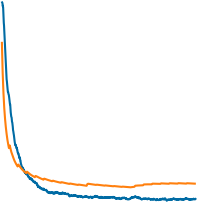
\includegraphics[interpolate=true,width=1.960000in,height=1.110000in]{sample-10000-img1.png}}%
\end{pgfscope}%
\begin{pgfscope}%
\pgfsetrectcap%
\pgfsetmiterjoin%
\pgfsetlinewidth{1.254687pt}%
\definecolor{currentstroke}{rgb}{0.150000,0.150000,0.150000}%
\pgfsetstrokecolor{currentstroke}%
\pgfsetdash{}{0pt}%
\pgfpathmoveto{\pgfqpoint{3.371599in}{0.558892in}}%
\pgfpathlineto{\pgfqpoint{3.371599in}{1.772367in}}%
\pgfusepath{stroke}%
\end{pgfscope}%
\begin{pgfscope}%
\pgfsetrectcap%
\pgfsetmiterjoin%
\pgfsetlinewidth{1.254687pt}%
\definecolor{currentstroke}{rgb}{0.150000,0.150000,0.150000}%
\pgfsetstrokecolor{currentstroke}%
\pgfsetdash{}{0pt}%
\pgfpathmoveto{\pgfqpoint{5.495496in}{0.558892in}}%
\pgfpathlineto{\pgfqpoint{5.495496in}{1.772367in}}%
\pgfusepath{stroke}%
\end{pgfscope}%
\begin{pgfscope}%
\pgfsetrectcap%
\pgfsetmiterjoin%
\pgfsetlinewidth{1.254687pt}%
\definecolor{currentstroke}{rgb}{0.150000,0.150000,0.150000}%
\pgfsetstrokecolor{currentstroke}%
\pgfsetdash{}{0pt}%
\pgfpathmoveto{\pgfqpoint{3.371599in}{0.558892in}}%
\pgfpathlineto{\pgfqpoint{5.495496in}{0.558892in}}%
\pgfusepath{stroke}%
\end{pgfscope}%
\begin{pgfscope}%
\pgfsetrectcap%
\pgfsetmiterjoin%
\pgfsetlinewidth{1.254687pt}%
\definecolor{currentstroke}{rgb}{0.150000,0.150000,0.150000}%
\pgfsetstrokecolor{currentstroke}%
\pgfsetdash{}{0pt}%
\pgfpathmoveto{\pgfqpoint{3.371599in}{1.772367in}}%
\pgfpathlineto{\pgfqpoint{5.495496in}{1.772367in}}%
\pgfusepath{stroke}%
\end{pgfscope}%
\begin{pgfscope}%
\pgfsetroundcap%
\pgfsetroundjoin%
\pgfsetlinewidth{1.505625pt}%
\definecolor{currentstroke}{rgb}{0.400000,0.760784,0.647059}%
\pgfsetstrokecolor{currentstroke}%
\pgfsetdash{}{0pt}%
\pgfpathmoveto{\pgfqpoint{4.535231in}{1.210150in}}%
\pgfpathlineto{\pgfqpoint{4.646342in}{1.210150in}}%
\pgfpathlineto{\pgfqpoint{4.757454in}{1.210150in}}%
\pgfusepath{stroke}%
\end{pgfscope}%
\begin{pgfscope}%
\definecolor{textcolor}{rgb}{0.150000,0.150000,0.150000}%
\pgfsetstrokecolor{textcolor}%
\pgfsetfillcolor{textcolor}%
\pgftext[x=4.846342in,y=1.171261in,left,base]{\color{textcolor}\rmfamily\fontsize{8.000000}{9.600000}\selectfont lstm train}%
\end{pgfscope}%
\begin{pgfscope}%
\pgfsetroundcap%
\pgfsetroundjoin%
\pgfsetlinewidth{1.505625pt}%
\definecolor{currentstroke}{rgb}{0.988235,0.552941,0.384314}%
\pgfsetstrokecolor{currentstroke}%
\pgfsetdash{}{0pt}%
\pgfpathmoveto{\pgfqpoint{4.535231in}{1.047064in}}%
\pgfpathlineto{\pgfqpoint{4.646342in}{1.047064in}}%
\pgfpathlineto{\pgfqpoint{4.757454in}{1.047064in}}%
\pgfusepath{stroke}%
\end{pgfscope}%
\begin{pgfscope}%
\definecolor{textcolor}{rgb}{0.150000,0.150000,0.150000}%
\pgfsetstrokecolor{textcolor}%
\pgfsetfillcolor{textcolor}%
\pgftext[x=4.846342in,y=1.008175in,left,base]{\color{textcolor}\rmfamily\fontsize{8.000000}{9.600000}\selectfont map train}%
\end{pgfscope}%
\begin{pgfscope}%
\pgfsetroundcap%
\pgfsetroundjoin%
\pgfsetlinewidth{1.505625pt}%
\definecolor{currentstroke}{rgb}{0.552941,0.627451,0.796078}%
\pgfsetstrokecolor{currentstroke}%
\pgfsetdash{}{0pt}%
\pgfpathmoveto{\pgfqpoint{4.535231in}{0.883979in}}%
\pgfpathlineto{\pgfqpoint{4.646342in}{0.883979in}}%
\pgfpathlineto{\pgfqpoint{4.757454in}{0.883979in}}%
\pgfusepath{stroke}%
\end{pgfscope}%
\begin{pgfscope}%
\definecolor{textcolor}{rgb}{0.150000,0.150000,0.150000}%
\pgfsetstrokecolor{textcolor}%
\pgfsetfillcolor{textcolor}%
\pgftext[x=4.846342in,y=0.845090in,left,base]{\color{textcolor}\rmfamily\fontsize{8.000000}{9.600000}\selectfont lstm test}%
\end{pgfscope}%
\begin{pgfscope}%
\pgfsetroundcap%
\pgfsetroundjoin%
\pgfsetlinewidth{1.505625pt}%
\definecolor{currentstroke}{rgb}{0.905882,0.541176,0.764706}%
\pgfsetstrokecolor{currentstroke}%
\pgfsetdash{}{0pt}%
\pgfpathmoveto{\pgfqpoint{4.535231in}{0.720893in}}%
\pgfpathlineto{\pgfqpoint{4.646342in}{0.720893in}}%
\pgfpathlineto{\pgfqpoint{4.757454in}{0.720893in}}%
\pgfusepath{stroke}%
\end{pgfscope}%
\begin{pgfscope}%
\definecolor{textcolor}{rgb}{0.150000,0.150000,0.150000}%
\pgfsetstrokecolor{textcolor}%
\pgfsetfillcolor{textcolor}%
\pgftext[x=4.846342in,y=0.682004in,left,base]{\color{textcolor}\rmfamily\fontsize{8.000000}{9.600000}\selectfont map test}%
\end{pgfscope}%
\begin{pgfscope}%
\definecolor{textcolor}{rgb}{0.150000,0.150000,0.150000}%
\pgfsetstrokecolor{textcolor}%
\pgfsetfillcolor{textcolor}%
\pgftext[x=2.822748in,y=2.213034in,,top]{\color{textcolor}\rmfamily\fontsize{12.000000}{14.400000}\selectfont 10000 training samples}%
\end{pgfscope}%
\end{pgfpicture}%
\makeatother%
\endgroup%

    \caption[Learning curves for varying training set sizes.]{Episode length and success rate curves for different training set sizes in terrain environment. Mean and standard deviation across 3 seeds.}
    \label{fig:sample}
\end{figure}
